\documentclass[pdflatex,sn-basic,Numbered]{sn-jnl}

\usepackage{microtype}
\usepackage{amsmath}
\usepackage[table]{xcolor}
\usepackage{booktabs}
\usepackage{threeparttable}
\usepackage{tabularx}
\usepackage{array}
\usepackage{xurl}
\usepackage{longtable}
\usepackage{fvextra}
\usepackage{placeins}
\setcounter{topnumber}{4}
\setcounter{bottomnumber}{3}
\setcounter{totalnumber}{6}
\renewcommand{\topfraction}{0.95}
\renewcommand{\bottomfraction}{0.85}
\renewcommand{\textfraction}{0.05}
\renewcommand{\floatpagefraction}{0.75}
% Permit in-text placement without changing any frozen table file or content.
\makeatletter
\let\JIISoriginaltable\table
\def\table{\@ifnextchar[{\JIIStable}{\JIISoriginaltable[htbp]}}
\def\JIIStable[#1]{\JIISoriginaltable[htbp]}
\expandafter\let\expandafter\JIISoriginaltablestar\csname table*\endcsname
\@namedef{table*}{\@ifnextchar[{\JIIStablestar}{\JIISoriginaltablestar[htbp]}}
\def\JIIStablestar[#1]{\JIISoriginaltablestar[htbp]}
\setlength{\@fptop}{0pt}
\setlength{\@fpsep}{14pt}
\setlength{\@fpbot}{0pt plus 1fil}
\makeatother

\hypersetup{
  pdftitle={Supplementary Information: When Does HyDE-Style Query Expansion Help? Reliability Boundaries in Multi-Hop Intelligent Information Retrieval},
  pdfauthor={Shiyong Xiong; Xingyun Chen},
  pdfkeywords={intelligent information retrieval; retrieval-augmented generation; multi-hop question answering; query expansion; reproducibility}
}

\newcommand{\best}[1]{\cellcolor{gray!15}\textbf{#1}}
\newcommand{\SuppRef}[1]{\ref{#1}}
\newcounter{algorithm}
\renewcommand{\thealgorithm}{S\arabic{algorithm}}
\renewcommand{\thesection}{S\arabic{section}}
\renewcommand{\thesubsection}{S\arabic{section}.\arabic{subsection}}
\renewcommand{\thetable}{S\arabic{table}}
\renewcommand{\thefigure}{S\arabic{figure}}
\setcounter{tocdepth}{1}
\makeatletter
\renewcommand*\l@section{\@dottedtocline{1}{1.5em}{3em}}
\makeatother

\begin{document}

\begin{center}
{\Large Supplementary Information}\\[3pt]
{\large Online Resource 1}\\[6pt]
{\large When Does HyDE-Style Query Expansion Help? Reliability Boundaries in Multi-Hop Intelligent Information Retrieval}\\[6pt]
{\normalsize Journal of Intelligent Information Systems}\\[3pt]
{\normalsize Authors: Shiyong Xiong and Xingyun Chen}\\[2pt]
{\normalsize Affiliation: School of Computer Science and Technology,}\\
{\normalsize Chongqing University of Posts and Telecommunications,}\\
{\normalsize Chongqing 400065, China}\\[2pt]
{\normalsize Corresponding author: Shiyong Xiong; e-mail: \href{mailto:1771856981@qq.com}{1771856981@qq.com}}
\end{center}

\noindent
This supplement preserves protocols, paired statistics, prompts, provenance and sensitivity results. The navigation below separates research-question evidence from protocol and diagnostic details. Tables and sections have independent S-prefixed counters. Artifact paths are relative to the review repository. Available results do not complete the original external family or supply independent human validation.

\section*{Result and Protocol Navigation}
\noindent Historical results, post-hoc diagnostics and newly frozen experiments remain separate. Use the labeled sections and tables below to locate a claim and its limits; the contents list provides the full section sequence.

\begin{center}
\small
\begin{tabularx}{\textwidth}{>{\raggedright\arraybackslash}p{0.21\textwidth} >{\raggedright\arraybackslash}X >{\raggedright\arraybackslash}p{0.30\textwidth}}
\toprule
Question or check & Evidence to inspect & Location \\
\midrule
RQ1: expansion & Controlled comparisons, paired effects, query composition and overlap diagnostics & Sections~\ref{sec:supp_hotpotqa_paired_statistics}, \ref{sec:supp_answer_overlap_normalization}, \ref{sec:supp_controlled_corpus_core} \\
RQ2: generator & Fixed open-generator protocol, content strata and matched encoder sensitivity & Sections~\ref{supp:sec:open_weight_confirmatory_protocol}--\ref{sec:supp_plan_b_sensitivity} \\
RQ3: corpus/reader & Full-wiki and 2Wiki corpus-scale methods, news matrix and matched Dense comparisons & Sections~\ref{sec:ircot_fullwiki}, \ref{sec:supp_corpus_scale_stress}, \ref{sec:supp_mhrag_external}, \ref{sec:supp_priority_diagnostics} \\
RQ4: iteration & Cumulative round-prefix effects and call accounting & Section~\ref{sec:ircot_fullwiki}; Table~\ref{tab:ircot_round_budget} \\
Delivered evidence & Official sentence matching and actual character/token retention & Sections~\ref{sec:supp_sentence_audit}--\ref{sec:supp_priority_diagnostics} \\
Capability and selection & New question-only/gold controls; 64-question same-choice validation & Sections~\ref{sec:supp_reader_controls_new}--\ref{sec:supp_independent_validation_new} \\
Protocol and metrics & Source freeze, prompts, adapters and scoring conventions & Sections~\ref{sec:supp_configuration_provenance}, \ref{sec:supp_prompt_api}, \ref{sec:supp_metric_normalization} \\
Reproduction limits & Tested local capsule, excluded inputs and archive status & Section~\ref{sec:supp_code_artifact_availability} \\
\bottomrule
\end{tabularx}
\end{center}

\tableofcontents

\clearpage

\section{Configuration Provenance and Freezing Protocol}
\label{sec:supp_configuration_provenance}

The manuscript uses released IRCoT processed HotpotQA and 2WikiMultihopQA \texttt{test\_subsampled} splits under a processed local-corpus protocol. The following records separate retrieval-reader protocol choices from verifier-specific diagnostic choices by listing the selection source, the data inspected, and the artifact-level freeze evidence for each configuration. They do not claim that every design choice was selected using an independent development split. In particular, the $q+h$ row supports a narrower provenance claim: the final HyDE query composition was fixed before the reported $q$-only, $h$-only, and question-plus-rewrite diagnostic controls were generated and scored. Same-split diagnostic tuning is disclosed for the secondary verifier risk rules and guarded-merge policy.

\subsection{System-Configuration Reliability Boundary}
\label{supp:system_configuration_boundary}

The methodological contribution is an audit protocol for conditional system claims, not a new retrieval algorithm. We represent an evaluated configuration as
\[
\mathcal{S}=(G,F,\mathcal{C},\Sigma,R,B),
\]
where $G$ is the query-side generator, $F$ is the retriever and index, $\mathcal{C}$ is the corpus, $\Sigma$ is the evidence serializer, $R$ is the answer reader, and $B$ is the generation/retrieval-call budget. A query-expansion result identifies a contrast between two such configurations, not a component-independent property.

For paired questions $i=1,\ldots,n$ and configurations $A$ and $B$, the conditional effect for endpoint $x$ is
\[
\Delta_x(A,B)=\frac{1}{n}\sum_{i=1}^{n}\left[m_{x,i}(A)-m_{x,i}(B)\right],
\qquad x\in\{\mathrm{ret},\mathrm{ans},\mathrm{cost}\}.
\]
Here $\Delta_{\mathrm{ret}}$, $\Delta_{\mathrm{ans}}$, and $\Delta_{\mathrm{cost}}$ use complete-support retrieval, reader EM/F1, and calls, respectively. Reader transport is tested by the interaction $\Delta_{\mathrm{ans}}(A,B\mid R_1)-\Delta_{\mathrm{ans}}(A,B\mid R_2)$. Changes in direction, uncertainty, or interpretation motivate boundary inspection; formal decisions follow the declared adjusted-test rule. The complete audit protocol is given in Table~\ref{tab:reliability_boundary_protocol}.

\begin{table*}[t]
\centering
\caption{Reliability-boundary audit for generative query expansion. A method-level claim is transportable only across the system factors that are explicitly varied and for which the paired conclusion remains stable.}
\label{tab:reliability_boundary_protocol}
\scriptsize
\begin{threeparttable}
\setlength{\tabcolsep}{3pt}
\begin{tabularx}{\textwidth}{>{\raggedright\arraybackslash}p{0.13\textwidth} >{\raggedright\arraybackslash}p{0.27\textwidth} >{\raggedright\arraybackslash}p{0.25\textwidth} >{\raggedright\arraybackslash}X}
\toprule
Boundary factor & Frozen comparison & Descriptive inspection signal & Required interpretation \\
\midrule
Generator provenance & Hold retriever, corpus, serialization, and top-$k$ fixed while changing a revision-pinned generator. & The point estimate changes direction or the declared adjusted decision changes. & Report generator-conditioned estimates and decisions; a sign change alone does not establish an interaction. \\
Generated content & Stratify exact answer overlap; repeat on answer-absent and gold-aware scrubbed variants. & The gain concentrates in answer- or support-bearing generations. & Report an artifact-level effect; do not claim contamination-free improvement. \\
Corpus and scale & Compare processed candidate corpora, a question-independent processed pool, and a fixed full-wiki index. & Magnitude or ranking changes with candidate construction or collection scale. & Bound transfer to the evaluated collection and indexing protocol. \\
Evidence interface & Audit supporting titles, exact paragraphs, and retention after the actual reader serializer. & Retrieved support is removed or truncated before reading. & Separate retrieval failure from evidence-interface loss. \\
Reader & Freeze evidence and compare readers; test reader-by-method interactions. & Point-estimate rankings differ or a declared adjusted interaction test is significant. & Rankings motivate inspection; formal reader dependence requires the separately specified interaction test. \\
Operating budget & Record generation/retrieval calls and compare frozen round prefixes. & Gains depend on additional calls, documents, or unequal stopping behavior. & State the operating point and avoid a universal efficiency or stopping claim. \\
Comparator strength & Audit a fixed candidate pool with a revision-pinned learned cross-encoder and a separately labeled bi-encoder rescore. & Evidence coverage differs, or the adjusted answer decision remains unresolved. & Condition conclusions on the executed candidate generator, reranker, reader, and declared test family. \\
\bottomrule
\end{tabularx}
\begin{tablenotes}
\footnotesize
\item Inspection signals do not determine formal states. Eligible primary endpoints use declared Holm-adjusted paired tests; confidence intervals describe effect uncertainty. Interval exclusion alone, point-estimate rankings, and non-primary retention diagnostics cannot establish transport. The procedure assigns supported, rejected, or unresolved to observed registered edges without causal attribution when multiple components change.
\end{tablenotes}
\end{threeparttable}
\end{table*}

\FloatBarrier
\begingroup
\footnotesize
\setlength{\tabcolsep}{2pt}
\renewcommand{\arraystretch}{1.02}
\begin{longtable}{>{\raggedright\arraybackslash}p{0.17\textwidth}
                            >{\raggedright\arraybackslash}p{0.27\textwidth}
                            >{\raggedright\arraybackslash}p{0.26\textwidth}
                            >{\raggedright\arraybackslash}p{0.24\textwidth}}
\caption{Configuration provenance for the reported processed-data evaluation.}
\label{tab:configuration_provenance}\\
\toprule
Component & Selection basis & Data inspected & Frozen stage \\
\midrule
\endfirsthead
\multicolumn{4}{l}{\footnotesize\itshape Table~\thetable\ continued}\\
\toprule
Component & Selection basis & Data inspected & Frozen stage \\
\midrule
\endhead
\midrule
\multicolumn{4}{r}{\footnotesize Continued on next page}\\
\endfoot
\bottomrule
\endlastfoot
$q+h$ HyDE query composition & Chosen from the HyDE-style design rationale: keep the original question as an anchor and append a document-like hypothetical passage for dense retrieval. It is not claimed to be selected by optimizing over the reported $q$-only, $h$-only, or $q+\mathrm{rewrite}$ diagnostic rows. & Released processed-split schema and local retrieval artifacts were inspected to implement the pipeline. The reported $q$-only, $h$-only, and $q+\mathrm{rewrite}$ diagnostic results were generated after the final $q+h$ protocol was already in use. & Canonical $q+h$ HotpotQA retrieval and reader artifacts were frozen on 2026-07-04. Query-composition controls were added later: $q$-only and $h$-only on 2026-07-06, and $q+\mathrm{rewrite}$ on 2026-07-08. \\
HyDE prompt & Template asks for one concise hypothetical supporting passage for retrieval-query expansion. The design follows document-like HyDE-style expansion rather than a prompt search over final EM/F1. & Prompt-template design, released question text, and later generated-passage artifacts for answer-string-overlap auditing. Gold answers are retained for evaluation metadata but are not inserted into the prompt text. & Frozen before canonical HotpotQA HyDE generation. Prompt-builder and prompt-file hashes are reported in Table~\ref{tab:qwen_api_reproducibility}. \\
Rewrite prompt & Control prompt designed to spend one extra query-side Qwen3.7-Max call while producing a direct retrieval query rather than a document-like passage. & Same reported question set and control-design constraints. Gold answers are not inserted into prompt text. The prompt is a matched-call control, not an optimized alternative final method. & Frozen before query-reformulation generation and reader scoring on 2026-07-08 to 2026-07-09; prompt-builder hash is reported in Table~\ref{tab:qwen_api_reproducibility}. \\
Equal-budget query-form prompts & Post-hoc mechanism diagnostic added after the primary HotpotQA analysis to test whether document-like form remains useful at similar generated length and call budget. The four modes use a shared one-call, 40-word target, 35--45 word instruction window, and 64-token generation cap. & Primary HotpotQA results and the length-versus-form threat were inspected before designing this diagnostic. After the prompt family was fixed, the same templates and budgets were applied to HotpotQA and 2WikiMultihopQA without dataset-specific modification. Gold answers are retained as scoring metadata but are not inserted into prompt text. & Prompt JSONL files were generated on 2026-07-21. Full equal-budget Qwen3.7-Max generations were frozen on 2026-07-22 to 2026-07-23, followed by local BGE-base retrieval scoring on 2026-07-23. This row is a post-hoc robustness diagnostic, not part of the primary frozen study. \\
Reader prompt & Generic evidence-grounded short-answer prompt with common answer-type instructions for yes/no, location, date/age comparison, role/title, and answer-only formatting. & General multi-hop QA answer-format requirements and retrieved evidence serialization. The same reader prompt is used across retrieval variants and reused on 2WikiMultihopQA without dataset-specific retuning. The reader is not constrained to copy a contiguous evidence span. & Frozen before final reader prompt JSONL and answer artifacts were generated; prompt-builder hash is reported in Table~\ref{tab:qwen_api_reproducibility}. \\
Top-$k=10$ retrieval budget & Common evidence budget inherited from the processed-data retrieval-reader protocol and used for comparable retrieval metrics and reader prompts. & Released IRCoT processed-data format, local candidate-pool size, and prompt-length feasibility. & Applied uniformly to all reported methods and both datasets before final scoring; no method-specific top-$k$ tuning is reported. \\
900-character evidence truncation & Prompt-budget rule for comparable reader and verifier evidence blocks under hosted-model context limits. & Local corpus paragraph lengths and prompt serialization constraints were inspected during prompt construction. & Applied before final reader and verifier prompt JSONL artifacts were generated; the same limit is used for reader and verifier evidence blocks. \\
Verifier risk rules & Secondary verifier selection policy for likely format, alias, date, count, granularity, abstention, role/type, comparison, overlong-answer, and short-entity risks. & Same HotpotQA split diagnostics over canonical HyDE reader outputs and EM mismatches. This is disclosed as same-split verifier development, not as independent held-out tuning. & Frozen before final HotpotQA HyDE verifier prompt generation; applying the frozen policy selected 120 verifier cases. \\
Verifier prompt & Conservative JSON verifier prompt with \emph{keep} as default and a limited set of benchmark-style corrections. & Same HotpotQA verifier-development diagnostics and retrieved-evidence examples used to define safe correction categories. & Frozen before the 120 verifier calls; all 120 structured outputs are audited in Table~\ref{tab:qwen_api_reproducibility}. \\
Abstention guard & Deterministic merge rule to block a new abstention when the initial reader answer is not an abstention. & Same HotpotQA verifier diagnostics and prior harmful-abstention risk analysis. & Frozen before the final guarded merge. It is inactive on the final HyDE verifier outputs but retained as a preventative guard. \\
Numeric-unit guard & Deterministic merge rule to block unsupported additions of units to bare numeric answers. & Same HotpotQA verifier diagnostics and raw-verifier transition analysis, including observed correct-to-wrong numeric-unit expansions. & Frozen before the final guarded merge; the guard removes the observed correct-to-wrong transitions in the reported HyDE verifier reconstruction. \\
BGE-base stronger-encoder reproduction & Post-hoc sensitivity check asking whether the query-composition pattern persists with a stronger dense encoder. It is not used as a tuned replacement for the MiniLM primary protocol. & Primary MiniLM results and frozen generated query artifacts were inspected. The diagnostic changes the encoder to \texttt{BAAI/bge-base-en-v1.5} while keeping prompts, top-$k$, reader prompt, and local-corpus protocol fixed. & Added after the primary HotpotQA scoring pass; reported as a sensitivity analysis rather than a pre-specified primary configuration. \\
Gold-aware scrubbing and answer-overlap diagnostics & Post-hoc internal-validity diagnostics for query-side answer-string overlap and generated gold-evidence traces. & Generated hypothetical passages, gold answers, supporting titles, and frozen retrieval artifacts were inspected for diagnostic grouping or scrubbing. These analyses are not used to choose a new deployed prompt. & Added after the primary HotpotQA results to bound the answer-leakage explanation; reported as diagnostic evidence only. \\
Corpus-scale and hard-negative audits & Post-hoc retrieval-only stress tests for corpus size, added-gold-title leakage, near-duplicate overlap, and harder processed-train distractors. & Released evaluation corpus records, processed-train distractors, frozen query-generation artifacts, and BGE similarity scores were inspected. The hard-negative row samples from the audited processed-train 100k pool rather than full Wikipedia. & Corpus-scale stress artifacts were generated after the primary study; leakage-filtered and BGE-hard audit artifacts are retained under the corpus-scale audit directory. These rows test external-validity threats after the primary study. \\
Qwen-Turbo fixed-evidence reader check & Post-hoc targeted reader robustness check. It changes only the reader model over fixed equal-budget top-10 evidence rather than rerunning query generation or retrieval. & Equal-budget retrieval outputs for direct rewrite, keyword/entity expansion, and document-like passage were inspected; no new retrieval artifacts were selected based on Qwen-Turbo answer quality. & Qwen-Turbo answer artifacts were frozen on 2026-07-23 to 2026-07-25. The check is a limited second-reader readout, not a broad reader sweep or primary end-to-end claim. \\
\end{longtable}
\noindent\emph{Note.} This table separates selection basis, inspected data, and freeze stage. It does not claim that every configuration was selected on an independent development split. The primary MiniLM retrieval-reader comparison is artifact-frozen as the main study; BGE, equal-budget, scrubbing, corpus-scale, top-$k$, supporting-paragraph, and Qwen-Turbo rows are post-hoc sensitivity diagnostics; same-split tuning is explicitly limited to the secondary verifier selection and guarded-merge analysis.
\endgroup

\begin{sidewaystable}[p]
\centering
\caption{Dataset source and converted-artifact provenance for the processed local-corpus protocol.}
\label{tab:dataset_artifact_provenance}
\scriptsize
\setlength{\tabcolsep}{3pt}
\newcommand{\shafull}[4]{\begin{tabular}{@{}l@{}}\texttt{#1}\\\texttt{#2}\\\texttt{#3}\\\texttt{#4}\end{tabular}}
\newcommand{\repocommit}{\begin{tabular}{@{}l@{}}\texttt{github.com/}\\\texttt{StonyBrookNLP/ircot}\\commit:\\\texttt{3c1820f698eea5eed}\\\texttt{db4fba3c56b64c96}\\\texttt{1e063e4}\\\texttt{main}; 2024-06-11\end{tabular}}
\begin{tabularx}{\dimexpr\textheight-8pt\relax}{>{\raggedright\arraybackslash}p{0.10\textheight}
                            >{\raggedright\arraybackslash}p{0.22\textheight}
                            >{\raggedright\arraybackslash}p{0.18\textheight}
                            >{\raggedright\arraybackslash}p{0.20\textwidth}
                            >{\raggedright\arraybackslash}X}
\toprule
Dataset & Upstream repository and commit & Source file and local download & Raw SHA-256 & Converted JSONL SHA-256 \\
\midrule
HotpotQA &
\repocommit &
\begin{tabular}{@{}l@{}}\texttt{processed\_data/}\\\texttt{hotpotqa/}\\\texttt{test\_subsampled.jsonl}\\downloaded: 2026-06-30\\21:01:24\end{tabular} &
\shafull{729D8987560092C8}{476523488069E6FB}{9BD1527157DC0D7B}{FEBF3DDC336C558E} &
questions:
\shafull{23F4AD6F82182C1B}{FE34C7F42DA3E852}{125EA71B0B9138CC}{B3E1740B3501E8AA}
corpus:
\shafull{8B27434696F9AB47}{9EB7301B7CB51259}{FDFBD9C7CEA96D7A}{2A728B68F761ACB2} \\
\addlinespace
2Wiki &
\repocommit &
\begin{tabular}{@{}l@{}}\texttt{processed\_data/}\\\texttt{2wikimultihopqa/}\\\texttt{test\_subsampled.jsonl}\\downloaded: 2026-06-30\\21:01:21\end{tabular} &
\shafull{4948757B90627F40}{B77CD6BF81A62C1A}{7AD525D6A6A0C91B}{17A2E0E2FA88F5BC} &
questions:
\shafull{7E1871FE8813606A}{1E4FBE393A8A1C48}{CC67376CBB2E864F}{4F8926A37A3FF1C7}
corpus:
\shafull{CF7603B72D3B0BA0}{7F008C6FEEB281E}{2C63579098CF98F2}{C1E47E61F241069C0} \\
\bottomrule
\end{tabularx}
\begin{tablenotes}
\footnotesize
\item Converted artifacts are \texttt{questions.jsonl} and \texttt{corpus.jsonl} under \texttt{local-artifacts/datasets/ircot\_hotpotqa\_test500} and \texttt{local-artifacts/datasets/ircot\_2wikimultihopqa\_test500}. HotpotQA converted files have local timestamp 2026-06-30 21:17:21; 2WikiMultihopQA converted files have local timestamp 2026-07-04 22:15:50.
\item The conversion script is \texttt{src/data/prepare\_ircot\_hotpotqa.py}, SHA-256 prefix \texttt{C23D8CC9E6EB}. It reads each processed row's \texttt{contexts}, writes one question record with the first extracted answer and supporting-title list, and writes one paragraph-level corpus record per context with \texttt{doc\_id}, title, paragraph text, source question id, and \texttt{is\_supporting}. The local corpus is then formed as the within-dataset union of these question-level candidate pools.
\end{tablenotes}
\end{sidewaystable}


\FloatBarrier
\section{Open-Weight Confirmatory Protocol}
\label{supp:sec:open_weight_confirmatory_protocol}

The minimum open-weight enhancement is executed in the \texttt{agentic\_rag} environment with a locally cached or explicitly downloaded model snapshot.

The generator is \texttt{Qwen/Qwen2.5-7B-Instruct}.
It is pinned to revision:\par\noindent
{\scriptsize\texttt{fe11104b620d588ccc049ff6631dd3ea002e3d98}};
decoding is greedy with
seed 13 and \texttt{max\_new\_tokens=96}. The dense retriever is
\texttt{BAAI/bge-base-en-v1.5}, pinned to revision
\texttt{a5beb1e3e68b9ab74eb54cfd186867f64f240e1a}, using CLS pooling, L2
normalization, a 512-token input limit, and top-$k=10$.

The confirmatory conditions are listed explicitly below. Query2doc-style (4-shot adaptation) is implemented as a faithful adaptation of the published pseudo-document
idea with two deterministic HotpotQA and two deterministic 2WikiMultihopQA
training demonstrations per target prompt. The local pool is fixed to the first
256 eligible released-order training examples per dataset; two examples are
selected from each dataset by a target-dependent SHA-256 ranking rule. The
demonstration identifiers, prompt SHA-256, model revision, decoding settings, package versions, and elapsed time
are stored in the generation JSONL. The open tier is retrieval-stage only; answer
overlap and gold-content scrubbing are marked diagnostic only and are not used to
select a final method.

\begin{center}
\textbf{Open-weight confirmatory condition names.}\par\vspace{3pt}
\centering
\small
\begin{tabular}{ll}
\toprule
Condition & Role \\
\midrule
\texttt{dense\_bge} & Question-only reference \\
\texttt{open\_hyde\_standard} & Standard HyDE prompt \\
\texttt{open\_hyde\_evidence\_only} & Evidence-only HyDE prompt \\
\texttt{open\_query2doc\_4shot} & Query2doc-style (4-shot adaptation) \\
\bottomrule
\end{tabular}
\end{center}

The runner writes one JSONL row per question and condition under \path{local-artifacts/expert_systems_minimum}. Retrieval rows expose stable IDs, ranks, document IDs, titles, and scores for internal auditing. The public per-example export removes question text, answer text, prompt text, generated passages, credentials, request identifiers, and other unrestricted benchmark content while preserving the condition, model revision, and retrieved-document metadata. The validation script rejects duplicate IDs, missing ranks, non-finite scores, forbidden content keys, and unpinned generator revisions. Summary CSV files report paired bootstrap intervals with 10,000 resamples and exact paired tests only after all required rows are present.

The aggregate retrieval-stage results are reconstructed directly from the verified summary files in the release package. The main manuscript reports the primary retrieval metrics, registered paired deltas, confidence intervals, exact-answer overlap rates, and generated lengths. Table~\ref{tab:open_generator_leakage} reports the mutually exclusive gold-content strata and the original, answer-scrubbed, and gold-content-scrubbed retrieval diagnostics. The latter are diagnostic only and use gold information unavailable at deployment time.

\subsection{Independent Mistral Generator Check}

Standard HyDE generation is repeated with the following frozen model:
\begin{center}
\small\path{mistralai/Mistral-7B-Instruct-v0.3}\par
{\scriptsize\texttt{c170c708c41dac9275d15a8fff4eca08d52bab71}}
\end{center}
The prompt, greedy 96-token decoding limit, question order, BGE revision, serialization, corpus, and top-$k=10$ are held fixed. The 500-row output for each dataset has no missing generations or retrieval failures. Median generated lengths are 63 words on HotpotQA and 59 words on 2WikiMultihopQA. Paired bootstrap intervals use 10,000 resamples; exact McNemar tests for all-support outcomes are Holm-corrected across the four generator-family contrasts. Public per-example outputs and aggregate statistics are reconstructed from \path{artifacts/per_example/second_generator_bge} and \path{artifacts/summaries/second_generator_bge}.

\begin{sidewaystable}[p]
\centering
\caption{Generator-content diagnostics. Panel A fixes the hosted hypothetical passages and BGE-base retriever, then reports the pre-existing mutually exclusive content strata. Panel B reports open-generator strata and gold-aware retrieval diagnostics.}
\label{tab:open_generator_leakage}
\footnotesize
\setlength{\tabcolsep}{2.5pt}
\textbf{Panel A: frozen hosted passages, paired BGE-base retrieval}\\[2pt]
\begin{tabular}{lrrrrrl}
\toprule
Gold-content stratum & $N$ & Question only & Hosted HyDE & $\Delta$ all-hit@10 & 95\% CI & Warning \\
\midrule
Exact-answer present & 292 & 0.8973 & 0.9760 & +0.0788 & [0.0445, 0.1130] & -- \\
Alias/paraphrase proxy present & 22 & 0.9091 & 0.9545 & +0.0455 & [0.0000, 0.1364] & $N<30$ \\
Supporting entity/title present & 154 & 0.8961 & 0.8896 & -0.0065 & [-0.0584, 0.0455] & -- \\
No identifiable gold content & 32 & 0.6562 & 0.5312 & -0.1250 & [-0.2813, 0.0000] & -- \\
\bottomrule
\end{tabular}

\vspace{5pt}
\textbf{Panel B: pinned open-generator diagnostics}\\[2pt]
\begin{tabular}{lllrrrrrrrrr}
\toprule
Dataset & Condition & Ref. & Exact & Alias & Title-only & None & Original & Ans.-scrub. & Gold-scrub. & McNemar $p$ & Holm $p$ \\
\midrule
HotpotQA & Open HyDE & Dense & 117 & 7 & 276 & 100 & 0.8460 & 0.8420 & 0.8140 & 0.0114 & 0.0908 \\
HotpotQA & Evidence-only HyDE & Open HyDE & 126 & 8 & 257 & 109 & 0.8160 & 0.8120 & 0.7940 & 0.0167 & 0.1167 \\
HotpotQA & Query2doc-style (4-shot adaptation) & Dense & 117 & 7 & 279 & 97 & 0.8700 & 0.8680 & 0.8520 & 0.4177 & 1.0000 \\
\midrule
2Wiki & Open HyDE & Dense & 226 & 6 & 261 & 7 & 0.4920 & 0.4880 & 0.4660 & 0.2892 & 1.0000 \\
2Wiki & Evidence-only HyDE & Open HyDE & 216 & 11 & 271 & 2 & 0.4880 & 0.4820 & 0.4420 & 0.8679 & 1.0000 \\
2Wiki & Query2doc-style (4-shot adaptation) & Dense & 200 & 5 & 285 & 10 & 0.4880 & 0.4860 & 0.4660 & 0.1524 & 0.7620 \\
\bottomrule
\end{tabular}

\vspace{3pt}
\parbox{0.95\textheight}{\footnotesize\emph{Note.} Panel A uses 10,000 paired question-level bootstrap resamples with fixed four-group classification; groups were not merged after inspecting outcomes. The alias/proxy group is flagged because $N<30$. These overlap strata are diagnostic and do not prove or disprove parametric memory, paraphrase leakage, or provider-side contamination. Panel B's answer- and gold-content-scrubbed rows are offline diagnostics only; McNemar and Holm-adjusted $p$-values use each condition's registered reference.}
\end{sidewaystable}

\begin{table*}[t]
\centering
\caption{Generator, BGE-instruction, and reader-interaction robustness. Panel A holds BGE-base, corpus, and top-$k=10$ fixed. Panel B adds only BGE's registered query prefix. Panel C reports $(\Delta_{\mathrm{Qwen}}-\Delta_{\mathrm{Mistral}})$ on frozen full-wiki evidence.}
\label{tab:generator_reader_robustness}
\scriptsize
\setlength{\tabcolsep}{3.5pt}
\textbf{A. Same-BGE generator sensitivity}\par\vspace{2pt}
\begin{tabular}{llrrrrl}
\toprule
Dataset & Query generator & $n$ & All-support & Recall & Delta & 95\% CI \\
\midrule
HotpotQA & Dense (no generator) & 500 & 0.8820 & 0.9380 & -- & -- \\
HotpotQA & Hosted alias & 500 & 0.9200 & 0.9570 & +0.0380 & [0.0100, 0.0660] \\
HotpotQA & Qwen2.5-7B & 500 & 0.8460 & 0.9180 & -0.0360 & [-0.0620, -0.0100] \\
HotpotQA & Mistral-7B-v0.3 & 500 & 0.8480 & 0.9190 & -0.0340 & [-0.0640, -0.0060] \\
\midrule
2Wiki & Dense (no generator) & 500 & 0.5100 & 0.7655 & -- & -- \\
2Wiki & Hosted alias & 500 & 0.7800 & 0.9130 & +0.2700 & [0.2300, 0.3120] \\
2Wiki & Qwen2.5-7B & 500 & 0.4920 & 0.7495 & -0.0180 & [-0.0480, 0.0120] \\
2Wiki & Mistral-7B-v0.3 & 500 & 0.5100 & 0.7545 & 0.0000 & [-0.0320, 0.0320] \\
\bottomrule
\end{tabular}

\vspace{5pt}
\textbf{B. BGE query-instruction sensitivity}\par\vspace{2pt}
\begin{tabular}{llrrrrr}
\toprule
Dataset & Query composition & No prefix & Prefix & Delta & 95\% CI & $p_{\mathrm{Holm}}$ \\
\midrule
HotpotQA & Question only & 0.882 & 0.882 & 0.000 & [-0.010, 0.010] & 1.0000 \\
HotpotQA & Question + Qwen HyDE & 0.846 & 0.836 & -0.010 & [-0.024, 0.002] & 0.7183 \\
2Wiki & Question only & 0.510 & 0.502 & -0.008 & [-0.020, 0.004] & 0.7183 \\
2Wiki & Question + Qwen HyDE & 0.492 & 0.504 & +0.012 & [-0.002, 0.028] & 0.7183 \\
\bottomrule
\end{tabular}

\vspace{5pt}
\textbf{C. Reader-by-method interaction}\par\vspace{2pt}
\begin{tabular}{lrrrrrr}
\toprule
Method contrast & EM int. & 95\% CI & $p_{\mathrm{Holm}}$ & F1 int. & F1 95\% CI & $n$ \\
\midrule
HyDE $-$ OneR & -0.006 & [-0.032, 0.022] & 0.7709 & -0.0156 & [-0.0457, 0.0143] & 500 \\
IRCoT $-$ OneR & +0.030 & [-0.004, 0.066] & 0.2562 & +0.0305 & [-0.0046, 0.0652] & 500 \\
IRCoT $-$ HyDE & +0.036 & [-0.004, 0.074] & 0.2562 & +0.0461 & [0.0078, 0.0853] & 500 \\
\bottomrule
\end{tabular}
\par\smallskip
\parbox{0.97\textwidth}{\footnotesize Panel B uses exact McNemar tests for all-support hit@10, Holm-adjusted across four contrasts. Panel C uses exact sign-flip tests for EM, Holm-adjusted across three method pairs. F1 intervals were registered without a separate significance decision.}
\end{table*}


\subsection{Query2doc-Style Transfer Protocol}
\label{supp:sec:query2doc_style_protocol}

The reader-facing name \emph{Query2doc-style (4-shot adaptation)} is used throughout this submission. The internal artifact key remains \texttt{open\_query2doc\_4shot} so that already frozen files and hashes remain stable. This condition is a faithful transfer of the published pseudo-document recipe for controlled comparison, but it is not an official reproduction. The original method and the present condition differ in task, benchmark corpus, demonstration pool, generator checkpoint, and dense retriever.

Each prompt contains four fixed query--passage demonstrations: two HotpotQA and two 2WikiMultihopQA training examples. For each dataset, the candidate demonstration pool is the first 256 eligible examples in released order. Target-specific demonstration IDs are selected deterministically by ranking SHA-256 hashes of the target ID, candidate ID, and seed 13. Test questions, test answers, test supporting-title labels, and test corpus passages are never used as demonstrations. The selected IDs and prompt SHA-256 are stored with every local generation row.

\begingroup\sloppy
The generator is \path{Qwen/Qwen2.5-7B-Instruct} at revision
\texttt{fe11104b620d588ccc049ff6631dd3ea002e3d98}. Greedy decoding uses
\texttt{do\_sample=false}, seed 13, and \texttt{max\_new\_tokens=96}. The
generated pseudo-document is serialized for retrieval as
\path{question [SEP] pseudo-document}. It is encoded with
\path{BAAI/bge-base-en-v1.5} at revision
\texttt{a5beb1e3e68b9ab74eb54cfd186867f64f240e1a}, CLS pooling, L2
normalization, a 512-token limit, and top-$k=10$. The pseudo-document is used
only to form the retrieval query and is never supplied to the downstream reader
as evidence.\par
\endgroup

No prompt, checkpoint, demonstration, or retrieval parameter is tuned on the 500-example test outputs. Because the transfer changes several components relative to the published Query2doc setting, results from this row support only a controlled neighboring-baseline comparison. They must not be interpreted as reproducing the original paper's absolute effectiveness.

\begin{table*}[t]
\centering
\caption{Open-weight retrieval-stage confirmatory results. Deltas and 95\% paired-bootstrap confidence intervals use each condition's pre-registered reference: Dense for standard HyDE and the Query2doc-style adaptation, and standard HyDE for evidence-only HyDE.}
\label{tab:open_generator_query2doc}
\scriptsize
\setlength{\tabcolsep}{3.0pt}
\textbf{A. Retrieval effectiveness}\par\smallskip
\begin{tabularx}{\textwidth}{l>{\raggedright\arraybackslash}Xrrlrr}
\toprule
Dataset & Condition & All-support & Recall & Reference & Delta & 95\% CI \\
\midrule
HotpotQA & Dense & 0.8820 & 0.9380 & -- & -- & -- \\
HotpotQA & Open HyDE & 0.8460 & 0.9180 & Dense & -0.0360 & [-0.0620, -0.0100] \\
HotpotQA & Evidence-only HyDE & 0.8160 & 0.9020 & Open HyDE & -0.0300 & [-0.0540, -0.0080] \\
HotpotQA & Query2doc-style (4-shot adaptation) & 0.8700 & 0.9320 & Dense & -0.0120 & [-0.0360, 0.0120] \\
\midrule
2Wiki & Dense & 0.5100 & 0.7655 & -- & -- & -- \\
2Wiki & Open HyDE & 0.4920 & 0.7495 & Dense & -0.0180 & [-0.0480, 0.0120] \\
2Wiki & Evidence-only HyDE & 0.4880 & 0.7390 & Open HyDE & -0.0040 & [-0.0280, 0.0180] \\
2Wiki & Query2doc-style (4-shot adaptation) & 0.4880 & 0.7505 & Dense & -0.0220 & [-0.0500, 0.0060] \\
\bottomrule
\end{tabularx}
\par\medskip
\textbf{B. Generation diagnostics}\par\smallskip
\begin{tabular}{llrr}
\toprule
Dataset & Condition & Exact-answer overlap & Mean words \\
\midrule
HotpotQA & Open HyDE & 0.2340 & 53.2 \\
HotpotQA & Evidence-only HyDE & 0.2520 & 71.6 \\
HotpotQA & Query2doc-style (4-shot adaptation) & 0.2340 & 34.6 \\
\midrule
2Wiki & Open HyDE & 0.4520 & 50.2 \\
2Wiki & Evidence-only HyDE & 0.4320 & 66.0 \\
2Wiki & Query2doc-style (4-shot adaptation) & 0.4000 & 33.5 \\
\bottomrule
\end{tabular}
\end{table*}


\subsection{Shared Question-Independent Corpus Check}
\label{supp:sec:shared_corpus_check}

The shared-corpus diagnostic removes per-question candidate-pool selection from the evaluated retrieval step. For each dataset, all selected questions and all methods use one audited 100k processed corpus. Added training records whose titles match test supporting titles are excluded. The corpus is still derived from processed benchmark artifacts rather than full Wikipedia.

\begin{table}[htbp]
\centering
\caption{Retrieval check on a shared question-independent 100k processed corpus. Each dataset uses a deterministic 200-question subset and a corpus shared across all selected questions; added training documents with test supporting titles are removed. Deltas use Dense as the paired reference.}
\label{tab:shared_corpus_check}
\footnotesize
\setlength{\tabcolsep}{1.5pt}
\begin{tabular}{llrrrrl}
\toprule
Dataset & Condition & $n$ & All-support & Recall & Delta & 95\% CI \\
\midrule
HotpotQA & Dense & 200 & 0.7150 & 0.8500 & -- & -- \\
HotpotQA & Hosted HyDE & 200 & 0.8450 & 0.9150 & 0.1300 & [0.0650, 0.1950] \\
HotpotQA & Open HyDE & 200 & 0.6650 & 0.8175 & -0.0500 & [-0.1050, 0.0050] \\
HotpotQA & Evidence-only open HyDE & 200 & 0.5950 & 0.7725 & -0.1200 & [-0.1800, -0.0600] \\
HotpotQA & Query2doc-style (4-shot adaptation) & 200 & 0.6600 & 0.8175 & -0.0550 & [-0.1050, -0.0050] \\
\midrule
2Wiki & Dense & 200 & 0.4050 & 0.7050 & -- & -- \\
2Wiki & Hosted HyDE & 200 & 0.6400 & 0.8400 & 0.2350 & [0.1700, 0.3000] \\
2Wiki & Open HyDE & 200 & 0.3450 & 0.6600 & -0.0600 & [-0.1050, -0.0200] \\
2Wiki & Evidence-only open HyDE & 200 & 0.3350 & 0.6175 & -0.0700 & [-0.1200, -0.0200] \\
2Wiki & Query2doc-style (4-shot adaptation) & 200 & 0.3550 & 0.6438 & -0.0500 & [-0.0900, -0.0150] \\
\bottomrule
\end{tabular}
\end{table}


\subsection{Hosted-Alias Temporal Drift Check}
\label{supp:sec:hosted_alias_drift}

The hosted-alias drift check replays a deterministic 50-question subset from each dataset against the currently configured hosted model alias, with three replays per question. The replay uses the original query-generation message shape and then reruns BGE-base retrieval from the replayed generated text. This check measures temporal sensitivity under the present alias; it does not reconstruct the historical provider-side snapshot used for the frozen primary artifacts. Because three replay rows share each selected question, the results are reported as descriptive agreement and similarity statistics rather than as independent inferential evidence.

\begin{table}[htbp]
\centering
\caption{Temporal sensitivity of the frozen hosted generations under a current-alias replay. Each dataset contributes 50 deterministic questions with three replays per question. Exact and text/embedding similarities compare replayed generations with the frozen originals; retrieval columns compare BGE-base top-10 outputs. This is not provider snapshot reconstruction.}
\label{tab:hosted_drift}
\scriptsize
\setlength{\tabcolsep}{3pt}
\begin{tabular}{lrrrrrrrr}
\toprule
Dataset & $n$ & Exact & Token J. & BGE cos. & Top-10 J. & Orig. all & Replay all & Agree \\
\midrule
HotpotQA & 150 & 0.0067 & 0.5811 & 0.9602 & 0.8104 & 0.9600 & 0.9600 & 1.0000 \\
2Wiki & 150 & 0.0000 & 0.5112 & 0.9307 & 0.6524 & 0.8000 & 0.7667 & 0.9667 \\
\bottomrule
\end{tabular}
\end{table}


\section{Post-Hoc and Pre-Output Sensitivity Analyses}
\label{sec:supp_plan_b_sensitivity}

The settings for these additional analyses were fixed on 16 August 2026 before their respective outputs were inspected, after the initial study. They are not preregistered or confirmatory evidence; retrospective input-evidence diagnostics are identified separately. The protocol fixes the original 500 IDs and order, seed 13, 10,000 question-level bootstrap resamples, exact paired tests for specified binary families, and no result-dependent tuning or row deletion. Aggregate release files are stored under \path{artifacts/summaries/jiis_revision}; private text-bearing rows remain outside the publication package.

\subsection{BGE Instruction Sensitivity}

The exact intervention is whether the query encoder receives \texttt{Represent this sentence for searching relevant passages:}. Document serialization and the cached document embeddings remain unchanged. HotpotQA and 2Wiki each contribute two instruction contrasts: question-only and question plus the frozen Qwen \texttt{open\_hyde\_standard} hypothetical passage. The four all-support McNemar tests form one Holm family. Instruction-minus-no-instruction changes are 0.000 and $-0.010$ on HotpotQA and $-0.008$ and $+0.012$ on 2Wiki; all four 95\% intervals include zero and all adjusted $p$-values are at least 0.7183. The exact generation-file hashes and encoder revision are recorded in the revision protocol and analysis manifest.

\subsection{Serialized Evidence Interface Audit}

The audit reuses the frozen OneR, HyDE, IRCoT, and BGE-base rescore retrieval rows and the aligned HotpotQA support contexts. A paragraph match requires equality of normalized title and complete normalized paragraph text. At top 10, all-support title and paragraph rates coincide at 0.298, 0.348, 0.354, and 0.460. The exact reader serializer retains only the first 450 characters per document; under the deliberately conservative requirement that every complete supporting paragraph remains verbatim, the rates fall to 0.112, 0.102, 0.140, and 0.176. Recomputing the interface at 900 characters yields 0.288, 0.332, 0.340, and 0.434. The aligned artifact lacks official sentence IDs. The separate retrospective audit in Section~\ref{sec:supp_sentence_audit} adds official sentence arrays; the original paragraph-label results above remain unchanged.

\subsection{Reader-by-Method Interaction}

For every method pair, the per-question interaction is $(\Delta_{\mathrm{Qwen}}-\Delta_{\mathrm{Mistral}})$. The headline IRCoT-minus-HyDE interaction is $+0.036$ EM (95\% CI $[-0.004,0.074]$; exact sign-flip $p_{\mathrm{Holm}}=0.2562$) and $+0.0461$ token F1 ($[0.0078,0.0853]$). The other two EM interaction intervals also include zero. F1 intervals were registered without a separate significance decision. Accordingly, the manuscript reports reader-specific point-estimate differences but does not claim a statistically established reader-dependent reversal.

\subsection{Full-Wiki Learned Reranker and Bi-Encoder Sensitivity}

The learned comparator uses question-only BM25 top-100 candidates followed by \texttt{BAAI/bge-reranker-v2-m3} reranking to top 10. The checkpoint is pinned to revision \texttt{953dc6f6f85a1b2dbfca4c34a2796e7dde08d41e}. The original 5,233,329-paragraph Elasticsearch index was restored locally, and all 500 top-100 candidate rows were exported. For every question, the first 10 candidates exactly match the frozen formal BM25 row. The candidate file contains 500 by 100 records and has SHA-256 \texttt{25b27bc9a7084fd29000d2665546b892e3ceda44a41c523df62eb7f5865f9f34}. The cross-encoder scored all 50,000 question--paragraph pairs and wrote 500 top-10 result rows.

The cross-encoder obtains any-hit/all-support/recall of 0.948/0.468/0.708. Its all-support differences versus OneR, HyDE, and IRCoT are $+0.170$ ($[0.136,0.206]$), $+0.120$ ($[0.076,0.162]$), and $+0.114$ ($[0.064,0.164]$); all three exact tests remain significant after Holm correction. With Qwen, its EM/F1 is 0.264/0.3480, and with Mistral it is 0.208/0.3476. Relative to OneR, the EM gains are $+0.044$ ($[0.014,0.074]$) and $+0.060$ ($[0.032,0.090]$), respectively. Relative to IRCoT, Qwen EM is unresolved, whereas Mistral EM is higher by $+0.048$ ($[0.014,0.082]$). The Qwen-minus-Mistral interaction for the gain over OneR crosses zero.

The separately labeled \texttt{BAAI/bge-base-en-v1.5} sensitivity control encodes the question and each candidate paragraph independently. It obtains any-hit/all-support/recall of 0.942/0.460/0.701 and Qwen EM/F1 of 0.270/0.3469. Its all-support difference from the cross-encoder is $-0.008$ ($[-0.020,0.002]$), so the learned comparator's incremental complete-support advantage is unresolved. This bi-encoder rescore remains useful for separating candidate-score strength from cross-encoding, but it is not relabeled as a learned cross-encoder.

\begin{table*}[t]
\centering
\caption{End-to-end work profile for the registered 500-question HotpotQA Full-Wiki conditions. Panel A reports mean structural work per question; Panel B reports total observed seconds and mean reader output tokens for each 500-question local-system stage. Missing historical reranker timing is reported as unavailable and is not imputed.}
\label{tab:fullwiki_system_cost}
\scriptsize
\textbf{Panel A: structural work per question}\\[2pt]
\setlength{\tabcolsep}{2.8pt}
\begin{tabular}{llrrrrrrr}
\toprule
Reader & Retrieval condition & $n$ & BM25 & Gen. & Gen. tok. & Rescore & Read calls & Fail \\
\midrule
Qwen & OneR/BM25 & 500 & 1.000 & 0.000 & 0.0 & 0.0 & 1.000 & 0 \\
Qwen & HyDE-BM25 & 500 & 1.000 & 1.000 & 73.4 & 0.0 & 1.000 & 0 \\
Qwen & IRCoT & 500 & 2.104 & 2.104 & 56.3 & 0.0 & 1.000 & 0 \\
Qwen & BGE-base & 500 & 1.000 & 0.000 & 0.0 & 100.0 & 1.000 & 0 \\
Qwen & BGE v2-m3 & 500 & 1.000 & 0.000 & 0.0 & 100.0 & 1.000 & 0 \\
\midrule
Mistral & OneR/BM25 & 500 & 1.000 & 0.000 & 0.0 & 0.0 & 1.000 & 0 \\
Mistral & HyDE-BM25 & 500 & 1.000 & 1.000 & 73.4 & 0.0 & 1.000 & 0 \\
Mistral & IRCoT & 500 & 2.104 & 2.104 & 56.3 & 0.0 & 1.000 & 0 \\
Mistral & BGE-base & 500 & 1.000 & 0.000 & 0.0 & 100.0 & 1.000 & 0 \\
Mistral & BGE v2-m3 & 500 & 1.000 & 0.000 & 0.0 & 100.0 & 1.000 & 0 \\
\bottomrule
\end{tabular}
\\[6pt]
\textbf{Panel B: observed runtime and reader output}\\[2pt]
\begin{tabular}{llrrr}
\toprule
Reader & Retrieval condition & Rerank s & Read tok. & Read s \\
\midrule
Qwen & OneR/BM25 & -- & 3.4 & 665.7 \\
Qwen & HyDE-BM25 & -- & 3.6 & 726.5 \\
Qwen & IRCoT & -- & 3.5 & 209.8 \\
Qwen & BGE-base & unavailable & 3.7 & 482.6 \\
Qwen & BGE v2-m3 & 972.5 & 3.8 & 1108.7 \\
\midrule
Mistral & OneR/BM25 & -- & 11.5 & 629.3 \\
Mistral & HyDE-BM25 & -- & 12.2 & 750.1 \\
Mistral & IRCoT & -- & 12.0 & 402.1 \\
Mistral & BGE-base & unavailable & 11.0 & 1550.0 \\
Mistral & BGE v2-m3 & 972.5 & 11.0 & 888.3 \\
\bottomrule
\end{tabular}
\\[3pt]\parbox{0.98\linewidth}{\footnotesize Qwen denotes Qwen2.5-7B-Instruct and Mistral denotes Mistral-7B-Instruct-v0.3. Gen. denotes retrieval-side generation; Read denotes the final answer reader. Rescore is the mean candidate count. Recorded reranker hardware: NVIDIA GeForce RTX 4060 Laptop GPU. Reader seconds are server-reported generation time; the historical row artifacts do not record an exact reader GPU. Times are therefore configuration-specific measurements, not hardware-independent efficiency or monetary cost.}
\end{table*}


\subsection{Independent 2Wiki Corpus-Scale Transport}

The independent tier freezes 428,395 unique paragraphs from the official 2Wiki train/dev/test context union in one question-independent Elasticsearch index. BM25, frozen Qwen-HyDE, official-code/open-Qwen IRCoT, and the same learned cross-encoder are evaluated on the same 500 released-order test questions; Qwen and Mistral read every frozen top-10 evidence file. The corpus hash is \texttt{000a99919ea821867ec4a50c2cc40e83da33eb4d5017799d24c51fa02bb283f8}. This split-union corpus is independently frozen but is not a second complete Wikipedia snapshot.

The cross-encoder has a positive retrieval point estimate over BM25, raising all-support hit@10 from 0.346 to 0.400 ($+0.054$; $[0.032,0.078]$), with a supported registered retrieval decision ($p_{\mathrm{Holm}}=2.23\times10^{-5}$). Qwen-HyDE reaches 0.356 ($+0.010$; $[-0.014,0.032]$), and IRCoT reaches 0.342 ($-0.004$; $[-0.052,0.042]$). The cross-encoder's answer gains over BM25 are unresolved with Qwen (EM $+0.014$; $[-0.016,0.044]$) and Mistral (EM $+0.008$; $[-0.012,0.028]$). Thus the observed 2Wiki retrieval increase receives a supported registered decision, whereas the answer edge remains unresolved.

\begin{table*}[t]
\centering
\caption{Transport check on the independent split-union corpus frozen from the official 2Wiki release. The corpus-scale tier is not a second complete Wikipedia snapshot.}
\label{tab:2wiki_corpus_scale}
\scriptsize
\setlength{\tabcolsep}{3pt}
\resizebox{\textwidth}{!}{%
\begin{tabular}{lrrrrrr}
\toprule
Method & All-support@10 & Recall@10 & Qwen EM & Qwen F1 & Mistral EM & Mistral F1 \\
\midrule
BM25 OneR & 0.346 & 0.671 & 0.212 & 0.224 & 0.052 & 0.164 \\
Qwen-HyDE & 0.356 & 0.665 & 0.186 & 0.209 & 0.056 & 0.162 \\
IRCoT + Qwen & 0.342 & 0.654 & 0.218 & 0.246 & 0.072 & 0.185 \\
BGE reranker v2-m3 & 0.400 & 0.705 & 0.226 & 0.244 & 0.060 & 0.172 \\
\bottomrule
\end{tabular}
}
\end{table*}


\FloatBarrier

\section{Official IRCoT Full-Wiki Retrieval and Reader Protocol}
\label{sec:ircot_fullwiki}

This tier vendors the official IRCoT repository at commit \texttt{3c1820f698eea5eeddb4fba3c56b64c961e063e4} and serves the fixed \texttt{Qwen/Qwen2.5-7B-Instruct} revision \texttt{fe11104b620d588ccc049ff6631dd3ea002e3d98} through a localhost-only compatibility endpoint. The HotpotQA full-wiki corpus is indexed once in Elasticsearch 7.10.2 and contains 5,233,329 paragraph documents. OneR/BM25, HyDE-BM25, and IRCoT share the same index and title--paragraph BM25 fields. The aligned evaluation list contains the same 500 HotpotQA IDs in the same order for every condition.

IRCoT uses the official prompt/orchestration boundary with a deterministic local generation adapter, a 2,000-token prompt budget, greedy decoding, and a maximum of 10 rounds. The output contract requests one next reasoning sentence per call. The formal stopping audit found natural terminal answers for 499 of 500 examples; one comparison question reached the 10-round hard cap after the private sentence-boundary adapter repeatedly split a legal-case abbreviation. The row is retained under the no-result-dependent-omission rule. Raw prompts, reasoning, paragraph text, and local request logs remain private, while the public 1,500-row export retains IDs, ranked document metadata, retrieval metrics, model/upstream revisions, and call counts.

\begin{table}[htbp]
\centering
\caption{Official-code deviation matrix for the HotpotQA full-wiki IRCoT tier.}
\label{tab:ircot_deviation_matrix}
\footnotesize
\setlength{\tabcolsep}{3pt}
\renewcommand{\arraystretch}{1.06}
\begin{tabularx}{\textwidth}{
  >{\raggedright\arraybackslash}p{0.14\textwidth}
  >{\raggedright\arraybackslash}p{0.35\textwidth}
  >{\raggedright\arraybackslash}X}
\toprule
Component & Frozen implementation & Relation to upstream or historical setup \\
\midrule
Upstream code & Official IRCoT commit \path{3c1820f698eea5eeddb4fba3c56b64c961e063e4}. & Retains the inference state machine and HotpotQA configuration generator. \\
Generator & Local Qwen2.5-7B-Instruct, pinned revision, NF4, greedy decoding, seed 13. & Replaces the historical generator; model-level equivalence is not claimed. \\
Compatibility alias & Upstream \texttt{flan-t5-base} API name retained only for routing; logs record Qwen. & Interface compatibility only, never reported as model identity. \\
\texttt{/generate/} service & Localhost adapter returns upstream-compatible generated text, token count, timing, and model fields. & Local compatibility implementation; no external API call. \\
Prompt handling & Official prompt text wrapped in a Qwen-Instruct chat template with a one-next-sentence instruction. & Required open-generator adaptation; model input is not byte-identical to the historical setup. \\
Token/decode limits & 2,000 input tokens, at most 200 new tokens per chain call, greedy decoding. & Reduces the upstream generated configuration's 6,000-token model limit. \\
Tokenizer hook & Official prompt reader loads the pinned local Qwen tokenizer through a scoped compatibility hook. & Test questions and retrieval logic are unchanged. \\
Sentence adapter & Lightweight \texttt{ircot-sentence-adapter-1} in the frozen primary run. & Replaces the historical spaCy runtime while preserving the controller interface. \\
Retrieval & Elasticsearch 7.10.2, official full-wiki schema, BM25 over title and paragraph, two documents per round. & Matches the selected official configuration and common frozen index. \\
Exit controls & Official controller, at most 10 reasoning sentences, \path{global_max_num_paras=15}. & Retained from the generated official configuration/runtime. \\
Evaluation subset & Frozen 500-question list; top-10 accumulated documents scored by supporting title. & Bounded confirmatory subset, not a full benchmark rerun. \\
\bottomrule
\end{tabularx}
\begin{tablenotes}
\footnotesize
\item Remaining differences include generator training data, Qwen chat serialization, tokenizer, quantized inference, package versions, and the sentence adapter. The label is official-code/open-generator adaptation, not exact historical reproduction.
\end{tablenotes}
\end{table}


Table~\ref{tab:ircot_fullwiki} reports all conditions and all predeclared contrasts. IRCoT improves all-support hit@10 over OneR/BM25, but it has lower any-hit than both baselines and lower supporting-title recall than HyDE-BM25. The tier is therefore evidence for an adaptive completeness/cost trade-off, not universal superiority. It is an official-code/open-generator adaptation and not an exact replay of the original IRCoT generator or its historical model behavior.

\begin{table}[htbp]
\centering
\caption{HotpotQA full-wiki retrieval with the official IRCoT code and a pinned local Qwen2.5-7B-Instruct generator. Panel A reports condition-level retrieval and call costs; Panel B reports target-minus-baseline all-support hit@10 contrasts with paired-bootstrap 95\% confidence intervals and Holm-adjusted exact McNemar tests. This is an official-code/open-generator adaptation, not an exact replay of the original generator.}
\label{tab:ircot_fullwiki}
\footnotesize
\setlength{\tabcolsep}{2pt}
\textbf{Panel A: conditions}\\[2pt]
\begin{tabular}{lrrrrrrr}
\toprule
Condition & $n$ & Any-hit & All-support & Recall & Ret. calls & Gen. calls & Hard cap \\
\midrule
OneR/BM25 & 500 & 0.8580 & 0.2980 & 0.5780 & 1.000 & 0.000 & 0 \\
HyDE-BM25 & 500 & 0.8760 & 0.3480 & 0.6120 & 1.000 & 1.000 & 0 \\
Official IRCoT + Qwen & 500 & 0.7960 & 0.3540 & 0.5750 & 2.104 & 2.104 & 1 \\
\bottomrule
\end{tabular}
\vspace{5pt}
\textbf{Panel B: paired all-support contrasts}\\[2pt]
\begin{tabular}{lrrrrr}
\toprule
Contrast & Delta & 95\% CI & Baseline only & Target only & Holm $p$ \\
\midrule
IRCoT $-$ OneR & 0.0560 & [0.0120, 0.1000] & 52 & 80 & 0.0369 \\
IRCoT $-$ HyDE & 0.0060 & [-0.0420, 0.0560] & 77 & 80 & 0.8732 \\
HyDE $-$ OneR & 0.0500 & [0.0160, 0.0840] & 28 & 53 & 0.0218 \\
\bottomrule
\end{tabular}
\par\vspace{3pt}\noindent\parbox{0.96\linewidth}{\footnotesize Hard-cap rows: 1/500. IRCoT used adaptive retrieval with a prespecified maximum of 10 generation rounds.}
\end{table}


\begin{table*}[t]
\centering
\caption{IRCoT round-budget sensitivity on the frozen 500-question HotpotQA full-wiki run. Prefixes are cumulative completed rounds, not strict equal-retrieval-budget systems. Reader scores use the pinned Qwen2.5-7B reader on each frozen prefix.}
\label{tab:ircot_round_budget}
\scriptsize
\setlength{\tabcolsep}{3.0pt}
\begin{tabular}{lrrrrrr}
\toprule
Stage & Mean ret. calls & Mean docs & All-support & Recall & EM & F1 \\
\midrule
Round 1 & 1.000 & 1.996 & 0.1580 & 0.4620 & 0.1660 & 0.2308 \\
Round 2 & 1.978 & 2.824 & 0.3440 & 0.5700 & 0.2540 & 0.3289 \\
Full adaptive run & 2.104 & 2.922 & 0.3540 & 0.5750 & 0.2620 & 0.3366 \\
\bottomrule
\end{tabular}
\par\smallskip
\begin{tabularx}{\textwidth}{llrr>{\raggedright\arraybackslash}Xrr}
\toprule
Contrast & Outcome & Delta & 95\% CI & Exact $p_{\mathrm{Holm}}$ & F1 delta & F1 95\% CI \\
\midrule
Round 1 $\rightarrow$ 2 & All-support & +0.1860 & [0.1520, 0.2200] & $4.04\!\times\!10^{-28}$ & +0.0981 & [0.0710, 0.1264] \\
Round 2 $\rightarrow$ full & All-support & +0.0100 & [0.0020, 0.0200] & 0.0625 & +0.0077 & [0.0017, 0.0154] \\
\bottomrule
\end{tabularx}
\end{table*}


\subsection{Full-Wiki Independent-Reader Protocol}

The three frozen 500-row retrieval files are read independently with two frozen
models:
\begin{center}
\small\path{Qwen/Qwen2.5-7B-Instruct}\par
{\scriptsize\texttt{fe11104b620d588ccc049ff6631dd3ea002e3d98}}\par\medskip
\small\path{mistralai/Mistral-7B-Instruct-v0.3}\par
{\scriptsize\texttt{c170c708c41dac9275d15a8fff4eca08d52bab71}}
\end{center}
Each question-condition-reader tuple receives one greedy call with seed 13,
\texttt{max\_input=2000}, and \texttt{max\_new\_tokens=32}. The shared prompt
contains the question and at most ten retrieved corpus paragraphs in rank order;
each paragraph is capped at 450 characters. It excludes gold aliases, support
flags, evaluation labels, HyDE pseudo-documents, retrieval queries, and IRCoT
reasoning traces.

A deterministic post-generation adapter maps a leading unknown or
insufficient-evidence response to \texttt{unknown}, removes an explicit
\texttt{Answer:} prefix, strips one enclosing quotation pair, and removes only
predefined trailing evidence or insufficiency explanations. The internal JSONL
retains the unchanged \texttt{raw\_prediction}; scoring uses the adapted
\texttt{prediction}. This amendment was frozen before the 500-row Mistral reader
runs and applied to all six reader conditions. Smoke outputs before the amendment
are archived separately and do not enter formal statistics.

EM and token F1 take the maximum over released gold aliases. Holm correction is
performed separately for the within-Qwen, within-Mistral, and cross-reader EM
families. Qwen EM/F1 is 0.2200/0.2815 for OneR, 0.2360/0.3017 for HyDE, and
0.2620/0.3366 for IRCoT. Mistral produces 0.1480/0.2674, 0.1700/0.3032, and
0.1600/0.2920, respectively. The public 3,000-row sensitivity export retains
stable IDs, condition labels, metrics, provenance, and call counts but omits
questions, aliases, prompts, raw or adapted predictions, titles, paragraph text,
URLs, endpoints, and reasoning. Source summaries are in
\path{artifacts/summaries/fullwiki_reader_sensitivity}.

\subsection{IRCoT Round-Prefix Sensitivity}

The frozen IRCoT trajectory is evaluated after round 1, after round 2, and at
natural or capped completion. For each prefix, retrieved documents are truncated
to the evidence available at that stage and the same Qwen reader is rerun. Round
1 averages 1.000 retrieval call and 1.996 documents; round 2 averages 1.978 calls
and 2.824 documents; the full trajectory averages 2.104 calls and 2.922 documents.
These prefixes therefore measure a round-budget frontier and are not strict
equal-budget conditions.

Paired comparisons are round 1 versus round 2 and round 2 versus full. Bootstrap
intervals use 10,000 resamples, and exact McNemar tests are Holm-corrected in
separate retrieval and answer families. All-support/EM/F1 are
0.158/0.166/0.2308 after round 1, 0.344/0.254/0.3289 after round 2, and
0.354/0.262/0.3366 at full exit. Sanitized per-example prefixes and summaries are
stored under \path{artifacts/per_example/ircot_round_budget} and
\path{artifacts/summaries/ircot_round_budget}.

\subsection{Post-Hoc Stopping Sensitivity}

The legal-abbreviation sensitivity is restricted to the retained hard-cap row
\texttt{5adcc9f35542990d50227d20}. Protecting \texttt{v.} from sentence-final
splitting reduces retrieval/generation rounds from 10 to 2 and generated tokens
from 316 to 50. Both versions retrieve both supporting titles, so any-hit,
all-support hit, and supporting-title recall remain 1.0. This post-hoc result
does not replace the frozen primary row and does not enter aggregate statistics.
The machine-readable comparison and source hashes are released in
\texttt{artifacts/summaries/ircot\_fullwiki/legal\_abbreviation\_sensitivity.json}.

\FloatBarrier

\section{Full HotpotQA Paired Statistics}
\label{sec:supp_hotpotqa_paired_statistics}

The HotpotQA paired statistics combine answer-side paired bootstrap/McNemar checks with retrieval-side paired checks over the same 500 examples. This table is the main supplemental lookup for the HotpotQA reliability claims in the manuscript.

\begin{sidewaystable}[p]
\centering
\caption{Full HotpotQA paired statistics on the released IRCoT \texttt{test\_subsampled} split.}
\label{tab:hotpotqa_paired_statistics}
\footnotesize
\setlength{\tabcolsep}{3pt}
\begin{tabularx}{\textheight}{>{\raggedright\arraybackslash}p{0.15\textheight}
                            >{\raggedright\arraybackslash}X
                            r r c c}
\toprule
Endpoint & Baseline $\rightarrow$ target & $\Delta$ metric 1 [95\% CI] & $\Delta$ metric 2 [95\% CI] & W$\rightarrow$C / C$\rightarrow$W & Test $p$ \\
\midrule
Answer EM/F1 & One-step Dense RAG $\rightarrow$ HyDE-style RAG & 0.0900 [0.0620, 0.1200] & 0.0906 [0.0634, 0.1192] & 53 / 8 & $<0.0001$ \\
Answer EM/F1 & Single-query Reformulation RAG $\rightarrow$ HyDE-style RAG & 0.0880 [0.0600, 0.1180] & 0.0976 [0.0690, 0.1266] & 52 / 8 & $<0.0001$ \\
Answer EM/F1 & Question + rewritten query $\rightarrow$ Question + hypothetical passage & 0.1040 [0.0740, 0.1340] & 0.1057 [0.0791, 0.1364] & 59 / 7 & $2.38{\times}10^{-11}$ \\
Answer EM/F1 & BM25 + Dense Hybrid $\rightarrow$ HyDE-style RAG & 0.0440 [0.0160, 0.0740] & 0.0529 [0.0264, 0.0803] & 37 / 15 & 0.0032 \\
Answer EM/F1 & Rule-based Evidence-Expanded Iterative Retrieval $\rightarrow$ HyDE-style RAG & 0.0480 [0.0220, 0.0740] & 0.0540 [0.0296, 0.0788] & 35 / 11 & 0.0005 \\
Answer EM/F1 & HyDE-style RAG $\rightarrow$ HyDE-style RAG + Conservative Verifier & 0.0040 [0.0000, 0.0100] & 0.0030 [0.0000, 0.0080] & 2 / 0 & 0.5000 \\
\midrule
Retrieval All/Recall & Dense RAG $\rightarrow$ HyDE-style RAG & 0.2380 [0.2000, 0.2780] & 0.1200 [0.1010, 0.1410] & 120 / 1 & $<0.0001$ \\
Retrieval All/Recall & Single-query Reformulation RAG $\rightarrow$ HyDE-style RAG & 0.2500 [0.2140, 0.2860] & 0.1290 [0.1090, 0.1500] & 125 / 0 & $<0.0001$ \\
Retrieval All/Recall & Question + rewritten query $\rightarrow$ Question + hypothetical passage & 0.2400 [0.2020, 0.2780] & 0.1250 [0.1060, 0.1470] & 123 / 3 & $<0.0001$ \\
Retrieval All/Recall & Hybrid RAG $\rightarrow$ HyDE-style RAG & 0.1200 [0.0840, 0.1560] & 0.0590 [0.0410, 0.0780] & 76 / 16 & $<0.0001$ \\
Retrieval All/Recall & Rule-based Evidence-Expanded Iterative Retrieval $\rightarrow$ HyDE-style RAG & 0.1140 [0.0780, 0.1480] & 0.0580 [0.0390, 0.0780] & 72 / 15 & $<0.0001$ \\
\bottomrule
\end{tabularx}
\begin{tablenotes}
\footnotesize
\item All rows use the same 500 paired HotpotQA examples. For answer rows, metric 1 is $\Delta$EM, metric 2 is $\Delta$F1, W$\rightarrow$C/C$\rightarrow$W count exact-match answer transitions, and $p$ is the exact McNemar test over discordant EM outcomes. For retrieval rows, metric 1 is $\Delta$all-support hit@10, metric 2 is $\Delta$supporting-title recall@10, W$\rightarrow$C/C$\rightarrow$W count target-only and baseline-only full-support retrieval, and $p$ is the exact McNemar test over full-support retrieval transitions. Intervals are paired bootstrap 95\% percentile intervals over per-example deltas.
\end{tablenotes}
\end{sidewaystable}


\section{2Wiki Paired Statistics}
\label{sec:supp_2wiki_paired_statistics}

The 2WikiMultihopQA split is reported as a secondary cross-dataset no-retuning check under the same processed local-corpus protocol, reader prompt, top-$k=10$ retrieval budget, and local candidate-pool setting. The paired rows reuse frozen answer and retrieval artifacts and are interpreted as secondary diagnostics.

\begin{sidewaystable}[p]
\centering
\caption{2WikiMultihopQA paired statistics and secondary absolute results.}
\label{tab:2wiki_paired_statistics}
\footnotesize
\setlength{\tabcolsep}{3pt}
\textit{Panel A: absolute retrieval-reader results.}
\begin{tabularx}{\textheight}{>{\raggedright\arraybackslash}X r r r r r}
\toprule
Method & Any hit@10 & All hit@10 & Recall@10 & EM & F1 \\
\midrule
One-step Dense RAG & 0.9840 & 0.3580 & 0.6695 & 0.5400 & 0.5767 \\
BM25 RAG & \best{0.9980} & 0.4320 & 0.7250 & 0.5840 & 0.6169 \\
BM25 + Dense Hybrid & \best{0.9980} & 0.4480 & 0.7330 & 0.5840 & 0.6220 \\
HyDE-style RAG & 0.9940 & \best{0.6680} & \best{0.8575} & \best{0.6620} & \best{0.7289} \\
\bottomrule
\end{tabularx}

\vspace{5pt}
\textit{Panel B: paired HyDE-over-baseline diagnostics.}
\begin{tabularx}{\textheight}{>{\raggedright\arraybackslash}X
                            r r c r r c}
\toprule
Baseline $\rightarrow$ target & $\Delta$EM [95\% CI] & $\Delta$F1 [95\% CI] & EM W$\rightarrow$C / C$\rightarrow$W & $\Delta$All@10 [95\% CI] & $\Delta$Recall@10 [95\% CI] & All@10 W$\rightarrow$C / C$\rightarrow$W \\
\midrule
Dense RAG $\rightarrow$ HyDE-style RAG & 0.1220 [0.0900, 0.1580] & 0.1523 [0.1186, 0.1881] & 72 / 11 & 0.3100 [0.2680, 0.3520] & 0.1880 [0.1665, 0.2085] & 157 / 2 \\
BM25 RAG $\rightarrow$ HyDE-style RAG & 0.0780 [0.0480, 0.1120] & 0.1121 [0.0793, 0.1450] & 54 / 15 & 0.2360 [0.1940, 0.2780] & 0.1325 [0.1115, 0.1550] & 133 / 15 \\
BM25 + Dense Hybrid $\rightarrow$ HyDE-style RAG & 0.0780 [0.0480, 0.1080] & 0.1069 [0.0751, 0.1399] & 53 / 14 & 0.2200 [0.1800, 0.2620] & 0.1245 [0.1020, 0.1475] & 125 / 15 \\
\bottomrule
\end{tabularx}
\begin{tablenotes}
\footnotesize
\item The 2WikiMultihopQA split is used as a secondary cross-dataset no-retuning check rather than as the main benchmark. Panel B uses the same 500 paired examples and frozen reader/retrieval artifacts. Answer-side intervals are paired bootstrap intervals over EM and F1 deltas; retrieval-side intervals are paired bootstrap intervals over all-support hit@10 and supporting-title recall@10 deltas. W$\rightarrow$C/C$\rightarrow$W count exact-match answer transitions for answer rows and target-only/baseline-only full-support retrieval for retrieval rows.
\end{tablenotes}
\end{sidewaystable}


\section{Deduplication Sensitivity}
\label{sec:supp_deduplication_sensitivity}

The local corpus for each dataset is the union of the released question-level candidate pools, indexed jointly within the dataset. Retrieval representations encode document titles and paragraph texts only. Question identifiers, supporting-evidence flags, gold answers, and evaluation metadata are retained for analysis but are not encoded by dense, BM25, or hybrid retrieval. Exact duplicate title--paragraph records are retained before indexing; if a paragraph appears in multiple question-level pools, each occurrence remains a separate document with a source-question-specific document identifier. Supporting-title metrics collapse duplicate retrieved titles before computing any-hit@10, all-hit@10, and supporting-title recall@10.

\begin{table*}[t]
\centering
\caption{Retrieval-side sensitivity to exact title--paragraph deduplication in the local joint index.}
\label{tab:dedup_retrieval_sensitivity}
\footnotesize
\begin{threeparttable}
\setlength{\tabcolsep}{2pt}
\begin{tabularx}{\textwidth}{>{\raggedright\arraybackslash}X l r r r r r r}
\toprule
Dataset & Method & Retain all@10 & Dedup all@10 & $\Delta$ all & Retain recall & Dedup recall & $\Delta$ recall \\
\midrule
HotpotQA & Dense & 0.6300 & 0.6320 & +0.0020 & 0.8080 & 0.8090 & +0.0010 \\
HotpotQA & Hybrid & 0.7480 & 0.7520 & +0.0040 & 0.8690 & 0.8710 & +0.0020 \\
HotpotQA & HyDE & 0.8680 & 0.8680 & +0.0000 & 0.9280 & 0.9280 & +0.0000 \\
2Wiki & Dense & 0.3580 & 0.3920 & +0.0340 & 0.6695 & 0.6920 & +0.0225 \\
2Wiki & Hybrid & 0.4480 & 0.4600 & +0.0120 & 0.7330 & 0.7415 & +0.0085 \\
2Wiki & HyDE & 0.6680 & 0.6760 & +0.0080 & 0.8575 & 0.8625 & +0.0050 \\
\bottomrule
\end{tabularx}
\begin{tablenotes}
\footnotesize
\item Retain duplicates uses the canonical joint local index with repeated title--paragraph records preserved. Dedup removes exact normalized title--paragraph duplicates before retrieval, then rebuilds dense, BM25, hybrid, and HyDE retrieval artifacts with the same top-$k=10$ setting. Metrics still collapse duplicate supporting titles during evaluation. Reader answers are not regenerated for the deduplicated indexes, so EM/F1 are not reported in this table.
\item The CSV artifact additionally reports average duplicate title slots and exact duplicate slots in the retrieved top-10 lists.
\end{tablenotes}
\end{threeparttable}
\end{table*}


The sensitivity table shows that exact title--paragraph deduplication leaves the method ordering unchanged. HotpotQA HyDE metrics remain unchanged, while all three tested methods improve slightly on 2WikiMultihopQA where repeated local-pool records occupy more top-10 slots. Reader answers are not regenerated for the deduplicated indexes, so this analysis should be read as a retrieval-side robustness check rather than an EM/F1 robustness check. We therefore keep the retained-duplicate joint index as the canonical protocol because it mirrors the released local-pool artifacts, and treat deduplication as a robustness check rather than a protocol change.

\FloatBarrier
\section{Guarded Answer Canonicalization Decomposition}
\label{sec:supp_verifier_guard_decomposition}

The verifier outputs are analyzed as a HyDE-native guarded answer-canonicalization layer. The decomposition below reuses the same HyDE reader answers and the same 120 risk-selected verifier outputs, then reconstructs raw merging and guarded merging policies without new model calls.

\begin{table*}[t]
\centering
\caption{HyDE verifier guard ablation reconstructed from existing verifier outputs.}
\label{tab:hyde_verifier_guard_ablation}
\small
\begin{threeparttable}
\begin{tabularx}{\textwidth}{>{\raggedright\arraybackslash}X r r r r r r c}
\toprule
Variant & $N$ & Verified & Changed & EM & F1 & $\Delta$F1 & W$\rightarrow$C / C$\rightarrow$W \\
\midrule
HyDE reader only & 500 & 0 & 0 & 0.6840 & 0.8105 & 0.0000 & 0 / 0 \\
HyDE + verifier raw & 500 & 120 & 5 & 0.6840 & 0.8119 & 0.0013 & 2 / 2 \\
HyDE + no-abstention guard & 500 & 120 & 5 & 0.6840 & 0.8119 & 0.0013 & 2 / 2 \\
HyDE + numeric-unit guard & 500 & 120 & 3 & 0.6880 & 0.8135 & 0.0030 & 2 / 0 \\
HyDE + both guards & 500 & 120 & 3 & 0.6880 & 0.8135 & 0.0030 & 2 / 0 \\
\bottomrule
\end{tabularx}
\begin{tablenotes}
\footnotesize
\item All rows reuse the same HyDE reader answers and the same 120 risk-selected verifier outputs. The raw row applies verifier final answers directly. The final row applies both deterministic guards: block new abstentions and block unsupported numeric-unit additions. The ablation is intended to justify the verifier's safety boundary, not to present verification as the main performance driver.
\end{tablenotes}
\end{threeparttable}
\end{table*}


\subsection{Guarded Merge Rule}
\label{sec:supp_guarded_merge_rule}

\refstepcounter{algorithm}
\noindent\textbf{Algorithm~\thealgorithm: Guarded canonicalization inference rule.}
\label{alg:guarded_canonicalization_rule}

\begin{enumerate}
    \item The reader receives the original question $q$ and retrieved corpus evidence $E$ and returns an initial short answer $a_0$.
    \item The rule-based selector computes a risk score $s(q,a_0)$. If $s(q,a_0)=0$, set the final answer $a_f=a_0$ and stop.
    \item If $s(q,a_0)>0$, query the conservative verifier with $(q,E,a_0)$ and parse its JSON output for the proposed final answer $\hat{a}$. If JSON parsing fails or the required answer field is missing, set $a_f=a_0$ and stop.
    \item Apply the abstention guard: if $a_0$ is not an abstention but $\hat{a}$ is an abstention, set $a_f=a_0$ and stop.
    \item Apply the numeric-unit guard: if $a_0$ is a bare number and $\hat{a}$ only appends a high-risk unit suffix, set $a_f=a_0$ unless the multi-word unit is explicitly requested by the question.
    \item Otherwise set $a_f=\hat{a}$.
\end{enumerate}
The final answer is therefore either the original reader answer or a selected-and-guarded verifier output for risk cases. The guard-decomposition table above reports the effect of raw merging and each deterministic guard using the same frozen verifier outputs.

\section{Full Call and Prompt-Character Accounting}
\label{sec:supp_full_accounting}

The main manuscript reports a compact LLM-call profile. The full accounting below separates query-side LLM calls, retrieval query executions, reader calls, verifier calls, total LLM calls, prompt-character proxies, evidence-character averages, and whether any method uses task-specific training. These are artifact-derived prompt-character and call-count statistics, not provider-side token, latency, or billing logs.

\begin{sidewaystable}[p]
\centering
\caption{Full structural call and retrieval-query accounting on the released IRCoT HotpotQA \texttt{test\_subsampled} split.}
\label{tab:efficiency_profile_full}
\footnotesize
\setlength{\tabcolsep}{3pt}
\begin{tabularx}{\textheight}{>{\raggedright\arraybackslash}X r r r r r r r}
\toprule
Method & Q-LLM/q & Ret.-q/q & Reader/q & Verifier/q & Total LLM/q & Prompt chars/q & Evidence chars/q \\
\midrule
LLM-only / No Retrieval & 0.00 & 0.00 & 1.00 & 0.00 & 1.00 & 368 & 0 \\
One-step Dense RAG & 0.00 & 1.00 & 1.00 & 0.00 & 1.00 & 6010 & 5149 \\
Multi-query RAG & 0.00 & 3.00 & 1.00 & 0.00 & 1.00 & 6010 & 5149 \\
Single-query Reformulation RAG & 1.00 & 1.00 & 1.00 & 0.00 & 2.00 & 6552 & 5169 \\
BM25 RAG & 0.00 & 1.00 & 1.00 & 0.00 & 1.00 & 6156 & 5295 \\
BM25 + Dense Hybrid & 0.00 & 2.00 & 1.00 & 0.00 & 1.00 & 5996 & 5135 \\
Rule-based Evidence-Expanded Iterative Retrieval & 0.00 & 4.00 & 1.00 & 0.00 & 1.00 & 6065 & 5204 \\
HyDE-style RAG & 1.00 & 1.00 & 1.00 & 0.00 & 2.00 & 6508 & 5121 \\
HyDE-style RAG + Guarded Canonicalization & 1.00 & 1.00 & 1.00 & 0.24 & 2.24 & 8214 & 5121 \\
\bottomrule
\end{tabularx}
\begin{tablenotes}
\footnotesize
\item Q-LLM/q counts query-side generation calls for matched-call reformulation or HyDE-style hypothetical-passage generation. Ret.-q/q counts retrieval query executions per question: Hybrid executes one dense and one BM25 retrieval, Multi-query executes three dense query variants, and Rule-based Evidence-Expanded Iterative Retrieval executes one first-round dense query plus three evidence-expanded dense queries. Total LLM/q counts query-side generation, reader answering, and selective verifier-backed canonicalization calls; it does not include retrieval query executions. Prompt chars/q reports average prompt characters per question from actual JSONL prompt files. Evidence chars/q reports serialized reader evidence length. The current logs do not store provider-side token usage, wall-clock latency, or billing. No method uses task-specific fine-tuning or model training.
\end{tablenotes}
\end{sidewaystable}


\begingroup
\footnotesize
\setlength{\tabcolsep}{3pt}
\begin{longtable}{>{\raggedright\arraybackslash}p{0.16\textwidth}
                            >{\raggedright\arraybackslash}p{0.27\textwidth}
                            >{\raggedright\arraybackslash}p{0.28\textwidth}
                            >{\raggedright\arraybackslash}p{0.22\textwidth}}
\caption{Implemented baseline and control retrieval parameters used in the frozen HotpotQA artifacts.}
\label{tab:baseline_implementation_parameters}\\
\toprule
Method & Query or document construction & Ranking and fusion rule & Frozen parameters and artifact notes \\
\midrule
\endfirsthead
\multicolumn{4}{l}{\footnotesize\itshape Table~\thetable\ continued}\\
\toprule
Method & Query or document construction & Ranking and fusion rule & Frozen parameters and artifact notes \\
\midrule
\endhead
\midrule
\multicolumn{4}{r}{\footnotesize Continued on next page}\\
\endfoot
\bottomrule
\endlastfoot
BM25 RAG & Query tokens are extracted from the original question by lowercasing and matching \texttt{[a-z0-9]+}. Each corpus record is represented as \texttt{title title text}, so the title receives a two-count lexical boost and the paragraph body appears once. & Standard BM25 lexical scoring with Robertson-style IDF, term-frequency saturation, and document-length normalization. No stopword removal, stemming, phrase matching, synonym expansion, or learned reranking is applied. & $k_1=1.5$, $b=0.75$, top-$k=10$. The retained-duplicate local index is used for the canonical table rows; the deduplicated variant is reported only in Table~\ref{tab:dedup_retrieval_sensitivity}. \\
BM25 + Dense Hybrid & The dense input list is the one-step \texttt{all-MiniLM-L6-v2} top-10 list; the lexical input list is the BM25 top-10 list above. Both lists contain title and paragraph text only, with analysis metadata excluded from retrieval representations. & Reciprocal-rank fusion over the two ranked lists: $\mathrm{score}(d)=I[d\in D]/(60+r_D(d))+I[d\in B]/(60+r_B(d))$. Missing-list contributions are zero; fused documents are sorted by this score. & Dense weight $=1.0$, BM25 weight $=1.0$, RRF constant $=60$, dense candidates $=10$, BM25 candidates $=10$, final top-$k=10$. No dense/BM25 raw-score calibration is used. \\
Multi-query RAG & Three deterministic query variants are built from the question: the original question, a capitalized-or-numeric entity-term query, and a non-stopword keyword query. A punctuation-normalized fallback is used only if fewer than three distinct variants are available. No LLM is used. & Each query is encoded with the same dense encoder and retrieves 10 candidates. Candidate lists are fused by weighted reciprocal-rank fusion, with query-index weights $0.5^j$ in the frozen HotpotQA artifact and RRF constant $60$; ties are broken by the best weighted dense similarity stored for the candidate. & Number of queries $=3$, per-query candidates $=10$, final top-$k=10$, \texttt{query\_decay}$=0.5$. The frozen artifact has the same top-10 document set as one-step Dense RAG for all 500 HotpotQA examples, but only 39/500 examples have the same order; reader context order can therefore change without adding new documents. \\
Rule-based Evidence-Expanded Iterative Retrieval & The first stage is the one-step dense top-10 retrieval. The second stage constructs four dense queries: the original question plus one expanded query for each of the first three first-round documents, formatted as the question, the related evidence title, and up to 700 characters of related evidence text. No reader output and no LLM call are used to form these queries. & The four dense queries each retrieve 10 candidates. Candidate documents are merged by document ID; each candidate keeps its maximum adjusted dense similarity, with weight $1.0$ for the original query and $0.97$ for evidence-expanded queries. The final list is sorted by the retained adjusted score. & First-round expansion documents $=3$, per-query candidates $=10$, retrieval query executions per question $=4$, final top-$k=10$. This is a fixed heuristic iterative control rather than a reproduction of IRCoT. The final top-10 is a re-ranked union of the second-stage candidate set, not a simple append to the first-stage list. \\
\end{longtable}
\noindent\emph{Note.} These rows describe the implemented retrieval baselines and controls used for the reported HotpotQA comparisons. Dense retrieval, Multi-query retrieval, Rule-based Evidence-Expanded Iterative Retrieval, and HyDE-style retrieval all use the same \path{sentence-transformers/all-MiniLM-L6-v2} encoder and normalized FAISS inner-product search unless a row states otherwise. Multi-query and Rule-based Evidence-Expanded Iterative Retrieval are fixed heuristic controls, and Single-query Reformulation is a matched-call mechanism control; they are not claimed as faithful public-method reproductions. The matched-call Single-query Reformulation and HyDE-style query prompts are specified in Section~\ref{sec:supp_prompt_api}.
\endgroup


\FloatBarrier
\section{Prompt and API Configuration}
\label{sec:supp_prompt_api}

This section gives the complete prompt templates used by the canonical query-side generation, matched-call query reformulation, equal-budget query-form diagnostic, evidence-grounded short-answer reader, and conservative verifier. The reader prompt uses generic short-answer formatting instructions for common multi-hop QA answer types and is applied unchanged to HotpotQA and 2WikiMultihopQA. The reader and verifier evidence blocks serialize the top-10 retrieved passages with title and paragraph text, truncated to at most 900 characters per document.

\subsection{HyDE Hypothetical-Passage Generation Prompt}
\begingroup\footnotesize
\begin{verbatim}
You are generating a hypothetical supporting passage for retrieval.
Given the question below, write a concise factual-sounding supporting passage
that would likely contain the answer.
The passage may be imperfect, but it should include key entities, relations,
and context useful for retrieving evidence.
Do not explain the task. Do not include bullet points. Write one short paragraph.

Question:
{question}

Hypothetical supporting passage:
\end{verbatim}
\endgroup

\subsection{Matched-Call Single-Query Reformulation Prompt}
\begingroup\footnotesize
\begin{verbatim}
You are rewriting a multi-hop question into a single retrieval query.
Given the question below, produce one concise search query for dense retrieval.
Use only entities, relations, and constraints already present in the question.
Do not answer the question. Do not add facts that are not stated in the question.
Do not write a paragraph or explanation. Output only the single retrieval query.

Question:
{question}

Single retrieval query:
\end{verbatim}
\endgroup

\subsection{Equal-Budget Query-Form Prompts and Serialization}
\label{sec:supp_equal_budget_prompts}

The equal-budget diagnostic reported in Tables~\ref{tab:equal_budget_retrieval_diagnostic} and~\ref{tab:equal_budget_reader_check} uses four separate query-form prompts with a shared wrapper. Each prompt asks for retrieval text, not an answer, uses one query-side generation call, targets 35--45 English words around a 40-word target, and sets the generation budget to \texttt{max\_tokens=64} with temperature 0. The prompt rows store gold answers and supporting-fact metadata only for later scoring; these fields are not inserted into the user prompt. We did not discard, truncate, or regenerate outputs solely because they fell outside the requested word window; the realized word counts are reported with the retrieval summary. Failed API requests are retried by the generation wrapper and, under \texttt{--resume}, rerun only as missing rows rather than replaced by hand-written text.

The generated text is used for retrieval only. For all four equal-budget rows, the BGE-base encoder input is the original question plus the generated retrieval text:
\begingroup\footnotesize
\begin{verbatim}
{question}

Generated retrieval text:
{generated_text}
\end{verbatim}
\endgroup
Thus, the document-like condition is encoded as $[q;G_{\mathrm{doc}}(q)]$, not as $G_{\mathrm{doc}}(q)$ alone. The exact separator is two newline characters, the label ``Generated retrieval text:'', and one newline before the model output. The BGE-base tokenizer then encodes this single serialized string with a 512-token query limit and right truncation. Lists, semicolons, bullets, and sentences are controlled only by the prompt text below: the keyword mode requests comma-separated phrases rather than sentences, the direct-rewrite mode requests one sentence, the decomposition mode requests numbered subquestions, and the document-like mode requests prose rather than bullets. The prompts do not include retrieved evidence or corpus text. They also do not impose a global ban on adding likely bridge concepts: the keyword/entity and document-like variants explicitly invite likely bridge concepts or plausible supporting context, while the direct-rewrite variant asks only to preserve the original intent and make implicit relations explicit.

\subsubsection*{Keyword/Entity Expansion}
\begingroup\footnotesize
\begin{Verbatim}[breaklines=true,breakanywhere=false,breaksymbolleft={},breaksymbolright={}]
You are generating retrieval text for a controlled multi-hop QA query-composition diagnostic.
Write a compact keyword/entity list for dense retrieval. Include entities, relations, constraints, and likely bridge concepts. Use comma-separated phrases, not sentences.

Use only one generation call. Do not answer the question. Do not explain the task.
Aim for 35-45 English words. Prefer concrete entities and relations over filler.
Output only the retrieval text.

Question:
{question}

Retrieval text:
\end{Verbatim}
\endgroup

\subsubsection*{Direct Rewrite}
\begingroup\footnotesize
\begin{Verbatim}[breaklines=true,breakanywhere=false,breaksymbolleft={},breaksymbolright={}]
You are generating retrieval text for a controlled multi-hop QA query-composition diagnostic.
Write one single dense-retrieval rewrite of the question. Preserve the original intent, make implicit relations explicit, and keep it as one sentence.

Use only one generation call. Do not answer the question. Do not explain the task.
Aim for 35-45 English words. Prefer concrete entities and relations over filler.
Output only the retrieval text.

Question:
{question}

Retrieval text:
\end{Verbatim}
\endgroup

\subsubsection*{Question Decomposition}
\begingroup\footnotesize
\begin{Verbatim}[breaklines=true,breakanywhere=false,breaksymbolleft={},breaksymbolright={}]
You are generating retrieval text for a controlled multi-hop QA query-composition diagnostic.
Write numbered subquestions that decompose the multi-hop question into retrieval steps. Keep the total output within the same length budget.

Use only one generation call. Do not answer the question. Do not explain the task.
Aim for 35-45 English words. Prefer concrete entities and relations over filler.
Output only the retrieval text.

Question:
{question}

Retrieval text:
\end{Verbatim}
\endgroup

\subsubsection*{Document-Like Passage}
\begingroup\footnotesize
\begin{Verbatim}[breaklines=true,breakanywhere=false,breaksymbolleft={},breaksymbolright={}]
You are generating retrieval text for a controlled multi-hop QA query-composition diagnostic.
Write one short encyclopedia-style passage that could plausibly support answering the question. Use prose rather than bullets.

Use only one generation call. Do not answer the question. Do not explain the task.
Aim for 35-45 English words. Prefer concrete entities and relations over filler.
Output only the retrieval text.

Question:
{question}

Retrieval text:
\end{Verbatim}
\endgroup

\subsection{Evidence-Grounded Short-Answer Reader Prompt}
The frozen prompt text below uses the historical word ``extractive'' in its system role. In this manuscript, this denotes evidence-constrained short-answer reading rather than standard span-extractive QA: the answer is not required to be a contiguous span copied from one evidence passage.
\begingroup\footnotesize
\begin{verbatim}
You are an extractive multi-hop question answering system.
Use only the evidence below. Combine facts across evidence items when needed.
Return the exact short answer phrase requested by the question.

Important rules:
- Return only the answer, with no explanation.
- Prefer the most specific answer phrase in the evidence.
- For yes/no questions, answer only "yes" or "no".
- For location questions, include the full location if the evidence gives it.
- For date/age comparison questions, the earlier birth date means the person is older.
- For role/position questions, return the exact position title, not a broader category.
- Do not answer "I don't know" if the evidence contains enough information to infer the answer.

Question:
{question}

Evidence:
{evidence}

Exact short answer:
\end{verbatim}
\endgroup

\subsection{Conservative Verification Prompt}
\begingroup\footnotesize
\begin{verbatim}
You are a conservative evidence-grounded answer verification agent.

Your default behavior is to KEEP the initial answer. Rewrite it only when there
is a clear benchmark-style formatting issue and the evidence directly supports
the corrected phrase.

Allowed corrections:
1. Nationality questions: prefer adjectival nationality when the evidence supports it.
   Example: "American" instead of "United States citizen".
2. Count questions: if the initial answer is only a number but the question asks
   for a counted object, include the unit from the evidence. Example:
   "12 member universities" instead of "12".
3. Date questions: if the question asks for an event time and the evidence gives
   a more complete month/year phrase, include the complete phrase.
4. Yes/no questions: if the question asks a yes/no comparison and the evidence
   directly supports it, normalize the answer to "Yes" or "No".
5. Abstained answers: if the initial answer is "I don't know" but the evidence
   directly contains the exact requested short answer, provide that answer.
   Otherwise keep "I don't know".
6. Location, role, title, or type questions: only add a missing qualifier when
   the question asks for that qualifier and the exact phrase appears in evidence.

Do not make these changes:
1. Do not abstain if the initial answer is directly supported by any evidence.
2. Do not expand a familiar short person name to a full legal name unless the
   question explicitly asks for the full name.
3. Do not remove location qualifiers such as state/country names.
4. Do not remove parenthetical title explanations.
5. Do not rewrite a correct answer merely because another phrase is also present.
6. Do not add units to a numeric answer when the question only asks for a number.
7. Do not replace a precise answer with a longer phrase unless the longer phrase
   is explicitly requested by the question.

Return only valid JSON with this exact schema:
{"verdict":"keep|correct|abstain","final_answer":"...","reason":"short reason"}

Question:
{question}

Initial answer:
{prediction}

Evidence:
{evidence}

JSON:
\end{verbatim}
\endgroup

\subsection{API, Model Invocation, and Result Ledger}

The hosted model is recorded at the artifact level because a third-party OpenAI-compatible relay exposes a mutable alias rather than a public immutable checkpoint. Code paths, ledger rows, and JSONL model fields retain the stored API alias \texttt{qwen3.7-max}; we do not infer a provider-side model identity from that alias. Reported reader, query-generation, and verifier artifacts use this stored API model string. The following tables freeze the local invocation windows, stored model fields, prompt hashes, retry policy, parsing policy, and raw-output boundaries.

\begingroup
\footnotesize
\setlength{\tabcolsep}{3pt}
\begin{longtable}{>{\raggedright\arraybackslash}p{0.18\textwidth}
                            >{\raggedright\arraybackslash}p{0.22\textwidth}
                            >{\raggedright\arraybackslash}p{0.17\textwidth}
                            >{\raggedleft\arraybackslash}p{0.12\textwidth}
                            >{\raggedright\arraybackslash}p{0.23\textwidth}}
\caption{Model invocation ledger for frozen hosted-Qwen artifacts.}
\label{tab:model_invocation_ledger}\\
\toprule
Artifact group & Local freeze window & Stored model field(s) & Calls / rows & Frozen artifact source \\
\midrule
\endfirsthead
\multicolumn{5}{l}{\footnotesize\itshape Table~\thetable\ continued}\\
\toprule
Artifact group & Local freeze window & Stored model field(s) & Calls / rows & Frozen artifact source \\
\midrule
\endhead
\midrule
\multicolumn{5}{r}{\footnotesize Continued on next page}\\
\endfoot
\bottomrule
\endlastfoot
HotpotQA retrieval baselines & 2026-07-02 to 2026-07-04 & \texttt{qwen3.7-max} & 5 $\times$ 500 & LLM-only, Dense, BM25, Hybrid, and Multi-query answer JSONL files. \\
HotpotQA matched-call query reformulation & 2026-07-08 to 2026-07-09 & \texttt{qwen3.7-max} & 3 $\times$ 500 & Single-query reformulation generation, rewritten-query reader, and question + rewritten-query reader JSONL files. \\
HotpotQA HyDE and iterative runs & 2026-07-04 to 2026-07-06 & \texttt{qwen3.7-max} & 4 $\times$ 500 & HyDE generation, HyDE reader, Rule-based Evidence-Expanded Iterative Retrieval reader, and HyDE hypothetical-only mechanism answer files. \\
HotpotQA conservative verifier & 2026-07-04 & \texttt{qwen3.7-max} & 120 verifier calls; 500 merged rows & Risk-selected verifier answer JSONL plus numeric-guarded merged evaluation file. \\
2WikiMultihopQA secondary runs & 2026-07-05 to 2026-07-06 & \texttt{qwen3.7-max} & 5 $\times$ 500 & 2Wiki Dense, BM25, Hybrid, HyDE generation, and HyDE reader answer files. \\
Equal-budget query-form generation & 2026-07-21 to 2026-07-23 & \texttt{qwen3.7-max} & 8 $\times$ 500 & Post-hoc HotpotQA and 2Wiki keyword/entity, direct-rewrite, question-decomposition, and document-like generation files. \\
Equal-budget Qwen-Turbo reader check & 2026-07-23 to 2026-07-25 & \texttt{qwen-turbo} & 6 $\times$ 500 & Direct-rewrite, keyword/entity-expansion, and document-like top-10 reader answer files for HotpotQA and 2Wiki. \\
\end{longtable}
\noindent\emph{Note.} All rows use a third-party OpenAI-compatible relay with temperature-0 decoding (\texttt{temperature=0.0}). The primary pipeline uses the stored API model string \texttt{qwen3.7-max}; the equal-budget query-form generation reuses \texttt{qwen3.7-max} as a post-hoc diagnostic; the targeted cross-reader check intentionally uses \texttt{qwen-turbo}. The aliases are artifact fields and do not establish provider-side model identity or an immutable snapshot. The configured \texttt{max\_tokens} budgets are reported separately as 64 for HyDE passage generation, equal-budget query-form generation, rewritten-query generation, reader answers, and verifier JSON output. Temperature 0 does not guarantee byte-identical replay across requests or hosted-model alias updates. Freeze windows are local artifact timestamps, not provider request logs. Table~\ref{tab:qwen_api_reproducibility} records the API-level reproducibility boundary, and the complete artifact-level ledger is recorded in \path{docs/model_invocation_ledger.md}.
\endgroup

\begingroup
\footnotesize
\setlength{\tabcolsep}{3pt}
\begin{longtable}{>{\raggedright\arraybackslash}p{0.20\textwidth}
                            >{\raggedright\arraybackslash}p{0.74\textwidth}}
\caption{Hosted Qwen API reproducibility record for frozen generation artifacts.}
\label{tab:qwen_api_reproducibility}\\
\toprule
Field & Frozen record or limitation \\
\midrule
\endfirsthead
\multicolumn{2}{l}{\footnotesize\itshape Table~\thetable\ continued}\\
\toprule
Field & Frozen record or limitation \\
\midrule
\endhead
\midrule
\multicolumn{2}{r}{\footnotesize Continued on next page}\\
\endfoot
\bottomrule
\endlastfoot
Provider and interface & Third-party OpenAI-compatible relay, accessed through the local \texttt{LLM\_BASE\_URL} environment variable. The relay operator and provider-side model identity were not independently verified; API credentials and endpoint URL are not stored in the artifact release. \\
API model string & Reported primary reader, query-generation, and verifier artifacts use the hosted API model string \texttt{qwen3.7-max}. The post-hoc equal-budget query-form generation also uses \texttt{qwen3.7-max}, while the targeted equal-budget reader robustness check uses \texttt{qwen-turbo} as a second hosted reader and is reported separately. The model string is stored in the local JSONL artifacts when the generation wrapper writes model metadata. \\
Snapshot/version & No immutable provider-side snapshot identifier was available for the hosted \texttt{qwen3.7-max} alias. Canonical runs are therefore frozen by local prompt and output artifacts rather than by a public model checkpoint. \\
Module model-string consistency & Primary HyDE generation, matched-call query reformulation, reader, 2Wiki, and verifier runs use the same API model string, \texttt{qwen3.7-max}. The post-hoc equal-budget query-form generation also uses \texttt{qwen3.7-max} but is not part of the primary frozen scoring window. The Qwen-Turbo check intentionally changes only the reader over fixed equal-budget retrieval evidence. Because these are hosted aliases rather than immutable snapshots, the paper does not claim replay against the exact same provider-internal model state after an alias evolves. \\
Experiment window & Primary Qwen3.7-Max artifacts were generated or frozen between 2026-07-02 and 2026-07-09 local time. Post-hoc equal-budget Qwen3.7-Max query-form generations were frozen between 2026-07-21 and 2026-07-23 local time. The targeted Qwen-Turbo fixed-evidence reader artifacts were frozen between 2026-07-23 and 2026-07-25 local time. Artifact-level windows and paths are listed in Table~\ref{tab:model_invocation_ledger}. \\
Endpoint region/type & Endpoint type is OpenAI-compatible \texttt{/v1} chat completions. Provider region was not exported into the local JSONL artifacts and is therefore not claimed as a reproducible field. \\
Temperature and output budgets & \texttt{temperature=0.0}. Configured \texttt{max\_tokens}: HyDE passage generation = 64; rewritten-query generation = 64; reader answer generation = 64; verifier JSON generation = 64. Temperature 0 is used to reduce sampling variation, but byte-identical replay is not claimed for a hosted alias. \\
\texttt{top\_p}, seed, and thinking mode & No \texttt{top\_p}, seed, logprob, response-format, or reasoning/thinking-mode parameter is explicitly sent by the wrapper, so provider defaults apply where relevant. Seed-controlled replay and thinking-mode equivalence are therefore not claimed. \\
Retry and timeout policy & Timeout is 60 seconds by default. Each request is attempted up to 3 times with 5 seconds between retries. If all retries fail, the script raises the final exception rather than writing a synthetic answer row. The \texttt{--resume} option skips completed IDs already present in the output JSONL and appends only missing rows. \\
API failure replacement policy & Reported \texttt{qwen3.7-max} HyDE, matched-call, 2Wiki, reader, and verifier runs, as well as the \texttt{qwen-turbo} fixed-evidence reader check, use completed rows from the frozen output files. Failed requests are rerun only as missing rows under \texttt{--resume}; they are not silently replaced by hand-written answers. \\
Prompt version/hash & Prompt-builder script SHA-256 prefixes: HyDE \texttt{89ECB4FB}, reader \texttt{98904C37}, query reformulation \texttt{FF9EA7EF}, equal-budget query-form \texttt{A234A00B}, verifier \texttt{BB2495BC}. Canonical HotpotQA prompt-file SHA-256 prefixes: HyDE generation \texttt{4D43047C}, HyDE reader \texttt{DCBC0B3E}, verifier risk-120 \texttt{763D188C}. Equal-budget prompt-file SHA-256 prefixes: HotpotQA keyword \texttt{048B13BE}, direct \texttt{2777A456}, decomposition \texttt{4244BD3E}, document-like \texttt{FF4A4ECF}; 2Wiki keyword \texttt{EC679B8B}, direct \texttt{E7464644}, decomposition \texttt{BF51AE1A}, document-like \texttt{CF15FFFD}. \\
Malformed JSON handling & Reader, HyDE, and query-reformulation generations are stored as raw text predictions and are not JSON-parsed. Verifier outputs are parsed as JSON when possible, with substring JSON extraction for wrapped responses. If verifier parsing fails, or if the parsed object lacks a nonempty \texttt{final\_answer} field, the fail-safe policy retains the initial reader answer $a_0$; malformed verifier text is never used as a candidate final answer. No automatic re-request is triggered solely by malformed JSON or JSON parse failure. \\
Verifier JSON parse audit & The canonical HotpotQA HyDE verifier artifact contains 120 verifier rows generated with \texttt{max\_tokens=64}. All 120 \texttt{prediction} fields were successfully parsed as direct JSON objects; substring fallback was used for 0 rows; final JSON parse failures were 0; empty verifier outputs were 0. All 120 verifier rows store the model field \texttt{qwen3.7-max}. The wrapper does not retain provider \texttt{finish\_reason} fields or per-request retry counters, and no automatic re-request rule is triggered solely by suspected output truncation. \\
Raw request/response retention & Local artifacts retain the full user prompt text, retrieved evidence, prediction text, model field, gold-answer metadata for scoring, and supporting-fact metadata. They do not retain the provider-side raw request envelope, raw response envelope, request IDs, token accounting, latency, billing, or per-request provider timestamps. Local artifact modification times provide freeze timestamps in the ledger. \\
\end{longtable}
\noindent\emph{Note.} Because the hosted model alias may evolve, all reported generations are accompanied by frozen raw prompts, local raw text outputs, local artifact freeze timestamps, and stored model strings. This table supports artifact-level reproducibility and rescoring, not exact replay of a provider-internal model snapshot or provider-side request log reconstruction.
\endgroup


For the structured verifier output, we audited the canonical HotpotQA HyDE verifier artifact
listed in Table~\ref{tab:model_invocation_ledger}.
All 120 verifier outputs were successfully parsed as direct JSON under the reported 64-token
budget. No substring JSON-recovery fallback was needed, no empty verifier output was observed,
and no final JSON parse failure remained in the frozen verifier artifact. The generation wrapper
does not store provider-side \texttt{finish\_reason} or per-request retry counters, so truncation
is bounded here by artifact-level parse success rather than by provider response metadata.

\subsection{Dense Encoder and Truncation Configuration}
\label{sec:supp_dense_encoder_truncation}

All canonical MiniLM-based dense retrieval variants use \path{sentence-transformers/all-MiniLM-L6-v2} through the \path{SentenceTransformer.encode} interface with normalized embeddings and FAISS inner-product search. The local audit environment reports \path{sentence-transformers==5.6.0}; the local MiniLM model cache records a \path{sentence_bert_config.json} value of \path{max_seq_length=256}. The underlying uncased BERT tokenizer uses WordPiece tokenization and the default Transformers truncation side is right truncation. Thus, MiniLM dense inputs are encoded as a single sequence with a shared 256-WordPiece-token budget, including the tokenizer's special tokens, and excess content is dropped from the right after serialization. The retained HotpotQA and 2Wiki MiniLM indexes are FAISS \path{IndexFlatIP} indexes over normalized 384-dimensional embeddings, so inner-product search is cosine-style nearest-neighbour retrieval.

The same tokenizer, 256-token budget, and right-truncation rule are applied to all dense query-composition diagnostic rows on HotpotQA: question only ($q$), single rewritten query ($r$), question plus rewritten query ($q+r$), hypothetical passage only ($h$), and question plus hypothetical passage ($q+h$). The generated text is character-capped before this tokenizer step: reformulated queries use at most 300 characters, and HyDE hypothetical passages use at most 900 characters with an ellipsis appended if capped. The combined rows share one encoder input sequence rather than separate per-field budgets for the question and generated text.

Dense query serialization is fixed by the retrieval scripts. The $q+h$ row serializes the original question, two newline characters, the label ``Hypothetical supporting passage:'', one newline, and the generated passage. The $q+r$ row uses the same layout with the label ``Rewritten retrieval query:''. The $q$, $r$, and $h$ rows encode only their corresponding serialized text. Corpus documents are serialized for dense indexing as \path{{title}. {paragraph}} and use the same 256-token right-truncation rule; there is no separate title or paragraph token budget. Question identifiers, support flags, answers, and evaluation metadata are not encoded.

All post-hoc BGE-base diagnostics use one frozen encoder configuration across the rows being compared:
\begin{itemize}
\item model identifier: \path{BAAI/bge-base-en-v1.5};
\item local Hugging Face \path{main} revision: \path{a5beb1e3e68b9ab74eb54cfd186867f64f240e1a};
\item local \path{model.safetensors} SHA-256 prefix: \path{C7C1988AAE20};
\item local \path{config.json} SHA-256 prefix: \path{BC00AF31A4A3};
\item local \path{tokenizer_config.json} SHA-256 prefix: \path{9261E7D79B44};
\item implementation: \path{transformers.AutoTokenizer} and \path{AutoModel}, not \path{SentenceTransformer.encode}; the local audit environment reports \path{transformers==4.57.6} and \path{torch==2.8.0}.
\end{itemize}

The BGE diagnostics use CLS pooling, taking \path{last_hidden_state[:, 0]} as the sequence embedding. Corpus-scale scripts expose a mean-pooling option for sensitivity work, but the reported BGE rows use the default \path{pooling=cls}. Both document and query inputs use \path{max_length=512}, tokenizer-side right truncation, and identical L2 normalization with \path{F.normalize(..., p=2, dim=1)}; this is equivalent to using normalized embeddings. The original BGE diagnostic rows encode plain serialized queries without the recommended instruction prefix. The additional instruction-prefix sensitivity in Section~\ref{sec:supp_plan_b_sensitivity} adds that exact prefix while holding document embeddings and all other encoder settings fixed.

BGE document serialization is \path{{title}. {paragraph_text}} with no separate title budget. The stronger-encoder query-composition diagnostic serializes question-only as $q$, single rewrite as $r$, hypothetical-only as $h$, and uses the following combined-query strings:
\begingroup\footnotesize
\begin{verbatim}
{question}\n\nRewritten retrieval query:\n{rewrite}

{question}\n\nHypothetical supporting passage:\n{hypothetical passage}
\end{verbatim}
\endgroup
The equal-budget diagnostic serializes each generated form identically as:
\begingroup\footnotesize
\begin{verbatim}
{question}\n\nGenerated retrieval text:\n{generated_text}
\end{verbatim}
\endgroup
Thus the document-like condition encodes $[q;G_{\mathrm{doc}}(q)]$ rather than $G_{\mathrm{doc}}(q)$ alone. BGE corpus-scale and hard-negative diagnostics use the same question-only, single-rewrite, and question-plus-hypothetical serializations as the stronger-encoder diagnostic. BGE diagnostics do not build a FAISS index: they compute dense score matrices as the dot product between L2-normalized query and document embeddings and select top-$k$ with \path{torch.topk}, making the score equivalent to cosine similarity.

\section{Corpus-Scale Retrieval Stress Test}
\label{sec:supp_corpus_scale_stress}

The main experiments use processed local candidate pools. To test sensitivity to a substantially noisier index without claiming full-wiki retrieval, we compare the original retained-duplicate local index with expanded 50k and 100k stress-test indexes. The expanded corpora preserve the released evaluation corpus and then add exact-title--paragraph-deduplicated distractor passages sampled from the corresponding IRCoT processed training split using seed 20260721. The expansion is gold-preserving by construction because the original evaluation support passages remain in the index; it is therefore a diagnostic retrieval stress test rather than a deployable retrieval protocol.

All rows use \texttt{BAAI/bge-base-en-v1.5}, CLS pooling, 512-token dense inputs, top-$k=10$, and the frozen question-only, single-query reformulation, and HyDE hypothetical-passage artifacts. No reader calls are rerun for this stress test. The script is \texttt{src/evaluation/analyze\_corpus\_scale\_retrieval\_stress.py}; the summary CSV, expanded corpora, retrieval JSONL files, and embedding caches are stored under \texttt{local-artifacts/corpus\_scale\_stress}. Paired bootstrap intervals are computed over per-example retrieval deltas.

\begin{sidewaystable}[p]
\centering
\caption{Full corpus-scale retrieval stress-test results. Local rows reuse the retained-duplicate BGE local-index artifacts from the main stronger-encoder reproduction table; only the 50k and 100k rows use newly expanded stress-test corpora.}
\label{tab:corpus_scale_stress_full}
\footnotesize
\setlength{\tabcolsep}{2.5pt}
\begin{tabularx}{\textheight}{l r >{\raggedright\arraybackslash}X r r r >{\raggedright\arraybackslash}X >{\raggedright\arraybackslash}X}
\toprule
Dataset & Docs & Query input & Any & All & Recall & HyDE delta vs. question & HyDE delta vs. rewrite \\
\midrule
HotpotQA & Local & Question only & 0.9940 & 0.8820 & 0.9380 & -- & -- \\
HotpotQA & Local & Single rewritten query & 0.9920 & 0.8340 & 0.9130 & -- & -- \\
HotpotQA & Local & Question + hypothetical passage & 0.9940 & \best{0.9200} & \best{0.9570} & All +0.0380 [0.0100, 0.0660]; recall +0.0190 [0.0050, 0.0340] & All +0.0860 [0.0560, 0.1160]; recall +0.0440 [0.0280, 0.0590] \\
\midrule
HotpotQA & 50k & Question only & 0.9820 & 0.7480 & 0.8650 & -- & -- \\
HotpotQA & 50k & Single rewritten query & 0.9720 & 0.6520 & 0.8120 & -- & -- \\
HotpotQA & 50k & Question + hypothetical passage & 0.9860 & \best{0.8560} & \best{0.9210} & All +0.1080 [0.0680, 0.1460]; recall +0.0560 [0.0350, 0.0770] & All +0.2040 [0.1620, 0.2440]; recall +0.1090 [0.0860, 0.1320] \\
\midrule
HotpotQA & 100k & Question only & 0.9800 & 0.6960 & 0.8380 & -- & -- \\
HotpotQA & 100k & Single rewritten query & 0.9680 & 0.5960 & 0.7820 & -- & -- \\
HotpotQA & 100k & Question + hypothetical passage & 0.9780 & \best{0.8340} & \best{0.9060} & All +0.1380 [0.1000, 0.1780]; recall +0.0680 [0.0470, 0.0890] & All +0.2380 [0.1940, 0.2800]; recall +0.1240 [0.0990, 0.1480] \\
\midrule
2Wiki & Local & Question only & 0.9980 & 0.5100 & 0.7655 & -- & -- \\
2Wiki & Local & Single rewritten query & 1.0000 & 0.4720 & 0.7380 & -- & -- \\
2Wiki & Local & Question + hypothetical passage & 1.0000 & \best{0.7800} & \best{0.9130} & All +0.2700 [0.2300, 0.3100]; recall +0.1475 [0.1290, 0.1675] & All +0.3080 [0.2680, 0.3520]; recall +0.1750 [0.1545, 0.1960] \\
\midrule
2Wiki & 50k & Question only & 1.0000 & 0.4460 & 0.7270 & -- & -- \\
2Wiki & 50k & Single rewritten query & 0.9960 & 0.4040 & 0.6900 & -- & -- \\
2Wiki & 50k & Question + hypothetical passage & 0.9980 & \best{0.6900} & \best{0.8655} & All +0.2440 [0.2040, 0.2840]; recall +0.1385 [0.1175, 0.1595] & All +0.2860 [0.2440, 0.3280]; recall +0.1755 [0.1545, 0.1980] \\
\midrule
2Wiki & 100k & Question only & 1.0000 & 0.4180 & 0.7105 & -- & -- \\
2Wiki & 100k & Single rewritten query & 0.9940 & 0.3600 & 0.6620 & -- & -- \\
2Wiki & 100k & Question + hypothetical passage & 0.9980 & \best{0.6500} & \best{0.8440} & All +0.2320 [0.1900, 0.2760]; recall +0.1335 [0.1110, 0.1560] & All +0.2900 [0.2460, 0.3340]; recall +0.1820 [0.1585, 0.2055] \\
\bottomrule
\end{tabularx}
\begin{tablenotes}
\footnotesize
\item Local denotes the original retained-duplicate local index used in the main stronger-encoder reproduction table (4,977 HotpotQA documents and 5,000 2Wiki documents). The rounded 5k stress-test cache is not used as a local-index replicate because the stress-construction script exact-deduplicates title--paragraph records before expansion and, for HotpotQA, pads the 4,977-document local corpus to 5,000 with train distractors. The 50k and 100k corpora preserve all released test-corpus records and add exact-title--paragraph-deduplicated contexts sampled from the corresponding IRCoT processed training split. All rows use \texttt{BAAI/bge-base-en-v1.5}, CLS pooling, 512-token dense inputs, top-$k=10$, and the frozen generated query artifacts used in the stronger-encoder reproduction. Deltas are computed only for the HyDE query row and use paired bootstrap 95\% confidence intervals over 500 per-example retrieval scores. The summary CSV is \texttt{local-artifacts/corpus\_scale\_stress/corpus\_scale\_retrieval\_summary.csv}; Local retrieval JSONL files are the stronger-encoder reproduction artifacts in \texttt{local-artifacts/results}, while expanded-corpus retrieval JSONL files and embedding caches are stored under \texttt{local-artifacts/corpus\_scale\_stress}. This gold-preserving distractor expansion is a diagnostic stress test and should not be interpreted as full-wiki retrieval.
\end{tablenotes}
\end{sidewaystable}


\FloatBarrier
\section{Detailed Retrieval and Reader Sensitivity Tables}
\label{sec:supp_detailed_sensitivity}

The following tables were moved from the main manuscript to keep the central argument within the journal page limit. They retain the frozen values and labels used by the earlier audit package. The stronger-encoder, equal-budget, corpus-scale, and top-$k$ rows are sensitivity analyses; they do not replace the predeclared primary conditions.

\begin{table*}[t]
\centering
\caption{Stronger dense-encoder query-composition sensitivity check with \texttt{BAAI/bge-base-en-v1.5}.}
\label{tab:stronger_encoder_reproduction}
\scriptsize
\begin{threeparttable}
\setlength{\tabcolsep}{3pt}
\begin{tabularx}{\textwidth}{l >{\raggedright\arraybackslash}X r r r r r}
\toprule
Dataset & Query used for dense retrieval & Any hit@10 & All hit@10 & Recall@10 & EM & F1 \\
\midrule
HotpotQA & Question only & \best{0.9940} & 0.8820 & 0.9380 & 0.6840 & 0.8153 \\
HotpotQA & Single rewritten query & 0.9920 & 0.8340 & 0.9130 & 0.6680 & 0.7965 \\
HotpotQA & Question + rewritten query & \best{0.9940} & 0.8520 & 0.9230 & 0.6760 & 0.8055 \\
HotpotQA & Hypothetical passage only & 0.9900 & 0.9080 & 0.9490 & \best{0.7040} & \best{0.8274} \\
\rowcolor{gray!10} HotpotQA & Question + hypothetical passage & \best{0.9940} & \best{0.9200} & \best{0.9570} & 0.7020 & 0.8267 \\
\midrule
2Wiki & Question only & 0.9980 & 0.5100 & 0.7655 & 0.6160 & 0.6609 \\
2Wiki & Single rewritten query & \best{1.0000} & 0.4720 & 0.7380 & 0.5840 & 0.6291 \\
2Wiki & Question + rewritten query & 0.9940 & 0.4540 & 0.7320 & 0.5940 & 0.6366 \\
2Wiki & Hypothetical passage only & \best{1.0000} & \best{0.8220} & \best{0.9275} & \best{0.6780} & \best{0.7459} \\
\rowcolor{gray!10} 2Wiki & Question + hypothetical passage & \best{1.0000} & 0.7800 & 0.9130 & 0.6740 & 0.7343 \\
\bottomrule
\end{tabularx}
\begin{tablenotes}
\footnotesize
\item All rows use BGE-base, top-$k=10$, the processed local-corpus protocol, and the same Qwen3.7-Max reader without retuning. Bold marks dataset-block maxima; shading marks the question + hypothetical serialization used by the primary MiniLM pipeline. This is a sensitivity check, not a tuned replacement for the main system.
\end{tablenotes}
\end{threeparttable}
\end{table*}

\begin{table*}[t]
\centering
\caption{Equal-budget BGE-base query-form diagnostic.}
\label{tab:equal_budget_retrieval_diagnostic}
\footnotesize
\begin{threeparttable}
\setlength{\tabcolsep}{3pt}
\renewcommand{\arraystretch}{1.05}
\textbf{(a) Absolute retrieval metrics.}
\smallskip
\begin{tabularx}{\textwidth}{l >{\raggedright\arraybackslash}X r r r r}
\toprule
Dataset & Generated query form & Mean words & Any hit@10 & All hit@10 & Recall@10 \\
\midrule
HotpotQA & Keyword/entity expansion & 38.370 & 0.9900 & 0.9240 & 0.9570 \\
HotpotQA & Direct rewrite & 39.392 & 0.9860 & 0.8800 & 0.9330 \\
HotpotQA & Question decomposition & 39.640 & 0.9900 & 0.8740 & 0.9320 \\
\rowcolor{gray!10} HotpotQA & Document-like passage & 39.246 & \best{0.9940} & \best{0.9260} & \best{0.9600} \\
\midrule
2Wiki & Keyword/entity expansion & 38.170 & 0.9920 & 0.6760 & 0.8410 \\
2Wiki & Direct rewrite & 39.628 & 0.9680 & 0.4760 & 0.7190 \\
2Wiki & Question decomposition & 40.008 & 0.9980 & 0.4540 & 0.7295 \\
\rowcolor{gray!10} 2Wiki & Document-like passage & 39.172 & \best{1.0000} & \best{0.7520} & \best{0.9035} \\
\bottomrule
\end{tabularx}
\medskip
\textbf{(b) Paired contrasts: document-like passage minus baseline.}
\smallskip
\begin{tabularx}{\textwidth}{l >{\raggedright\arraybackslash}X r r r}
\toprule
Dataset & Baseline form & $N$ & $\Delta$ All hit@10 [95\% CI] & $\Delta$ Recall@10 [95\% CI] \\
\midrule
HotpotQA & Direct rewrite & 500 & +0.0460 [+0.0200, +0.0720] & +0.0270 [+0.0120, +0.0410] \\
HotpotQA & Question decomposition & 500 & +0.0520 [+0.0260, +0.0800] & +0.0280 [+0.0140, +0.0430] \\
HotpotQA & Keyword/entity expansion & 500 & +0.0020 [-0.0180, +0.0220] & +0.0030 [-0.0080, +0.0140] \\
\midrule
2Wiki & Direct rewrite & 500 & +0.2760 [+0.2360, +0.3160] & +0.1845 [+0.1620, +0.2070] \\
2Wiki & Question decomposition & 500 & +0.2980 [+0.2580, +0.3420] & +0.1740 [+0.1530, +0.1940] \\
2Wiki & Keyword/entity expansion & 500 & +0.0760 [+0.0440, +0.1080] & +0.0625 [+0.0460, +0.0800] \\
\bottomrule
\end{tabularx}
\begin{tablenotes}
\footnotesize
\item Each row evaluates 500 examples with one Qwen3.7-Max generation call, a 40-word target, a 64-token cap, the same BGE-base encoder, and top-$k=10$. Retrieval encodes the original question plus generated text; reader answers are not regenerated. Bold marks dataset-block maxima, and shaded rows mark the document-like form. Panel (b) reports paired bootstrap 95\% percentile intervals ($B=2000$, seed 13). Prompt and serialization details are in Online Resource 1, Section~\ref{sec:supp_equal_budget_prompts}.
\end{tablenotes}
\end{threeparttable}
\end{table*}

\begin{table}[htbp]
\centering
\caption{Qwen-Turbo reader check on fixed equal-budget evidence.}
\label{tab:equal_budget_reader_check}
\footnotesize
\setlength{\tabcolsep}{3pt}
\renewcommand{\arraystretch}{1.08}

\begin{tabularx}{\textwidth}{@{}l>{\raggedright\arraybackslash}Xcc@{}}
\toprule
Dataset & Baseline $\rightarrow$ doc-like & \shortstack{Baseline\\EM / F1} & \shortstack{Doc-like\\EM / F1} \\
\midrule
HotpotQA & Direct rewrite $\rightarrow$ doc-like & \shortstack{0.4960\\0.6294} & \shortstack{0.5660\\0.7046} \\
HotpotQA & Keyword/entity expansion $\rightarrow$ doc-like & \shortstack{0.5500\\0.6777} & \shortstack{0.5660\\0.7046} \\
2Wiki & Direct rewrite $\rightarrow$ doc-like & \shortstack{0.3460\\0.4148} & \shortstack{0.3620\\0.4498} \\
2Wiki & Keyword/entity expansion $\rightarrow$ doc-like & \shortstack{0.3640\\0.4498} & \shortstack{0.3620\\0.4498} \\
\bottomrule
\end{tabularx}
\medskip\textbf{Paired differences}\par\smallskip
\begin{tabularx}{\textwidth}{@{}l>{\raggedright\arraybackslash}Xrcrc@{}}
\toprule
Dataset & Baseline $\rightarrow$ doc-like & $\Delta$EM & $\Delta$F1 [95\% CI] & \shortstack{W$\rightarrow$C /\\C$\rightarrow$W} & McNemar $p$ \\
\midrule
HotpotQA & Direct rewrite $\rightarrow$ doc-like & 0.0700 & \shortstack{0.0752\\\mbox{[0.0495, 0.1001]}} & 45 / 10 & $<0.0001$ \\
HotpotQA & Keyword/entity expansion $\rightarrow$ doc-like & 0.0160 & \shortstack{0.0269\\\mbox{[0.0053, 0.0503]}} & 24 / 16 & 0.2682 \\
2Wiki & Direct rewrite $\rightarrow$ doc-like & 0.0160 & \shortstack{0.0350\\\mbox{[0.0006, 0.0727]}} & 48 / 40 & 0.4557 \\
2Wiki & Keyword/entity expansion $\rightarrow$ doc-like & -0.0020 & \shortstack{0.0000\\\mbox{[-0.0354, 0.0342]}} & 36 / 37 & 1.0000 \\
\bottomrule
\end{tabularx}
\begin{tablenotes}
\footnotesize
\item All rows reuse the equal-budget BGE-base top-10 evidence and regenerate only reader answers with \texttt{qwen-turbo}. $\Delta$ values are document-like passage minus the named baseline over 500 paired examples. F1 intervals are paired bootstrap 95\% confidence intervals; W$\rightarrow$C and C$\rightarrow$W are EM transitions for document-like versus baseline.
\end{tablenotes}
\end{table}

\FloatBarrier
Table~\ref{tab:corpus_scale_stress_full} supplies the complete corpus-scale statistics, with construction details in Section~\ref{sec:supp_corpus_scale_stress}.
\begin{table*}[t]
\centering
\caption{Corpus-scale leakage and BGE hard-negative audit.}
\label{tab:corpus_scale_audit}
\footnotesize
\begin{threeparttable}
\setlength{\tabcolsep}{2.3pt}
\renewcommand{\arraystretch}{1.12}
\begin{tabularx}{\textwidth}{@{}l l r r r r r r r@{}}
\toprule
\multicolumn{2}{c}{Corpus} & \multicolumn{4}{c}{Added-distractor audit} & \multicolumn{3}{c}{All-support hit@10} \\
\cmidrule(lr){1-2}\cmidrule(lr){3-6}\cmidrule(lr){7-9}
Dataset & Stress corpus & Docs & \shortstack{Added\\gold titles} & \shortstack{Near-dup.\\support} & \shortstack{BGE sim.\\p95} & \shortstack{Question\\only} & HyDE & $\Delta$ \\
\midrule
HotpotQA & Random 100k & 100000 & 1 & 1 & 0.6011 & 0.6960 & 0.8340 & 0.1380 \\
HotpotQA & No-gold-title 100k & 99999 & 0 & 0 & 0.6011 & 0.6960 & 0.8340 & 0.1380 \\
HotpotQA & BGE-hard 50k & 50000 & 0 & 0 & 0.6204 & 0.6960 & 0.8420 & 0.1460 \\
2Wiki & Random 100k & 100000 & 173 & 173 & 0.5948 & 0.4180 & 0.6500 & 0.2320 \\
2Wiki & No-gold-title 100k & 99827 & 0 & 0 & 0.5948 & 0.4180 & 0.6520 & 0.2340 \\
2Wiki & BGE-hard 50k & 50000 & 0 & 0 & 0.6172 & 0.4180 & 0.6580 & 0.2400 \\
\bottomrule
\end{tabularx}
\begin{tablenotes}
\footnotesize
\item Random 100k audits the processed-train distractor expansion. No-gold-title removes only added train records whose normalized title matches a test supporting title. BGE-hard selects the most question-similar added train distractors from the audited 100k pool after that exclusion. BGE sim. p95 is the 95th percentile of each added distractor's maximum BGE cosine similarity to any test question; near-dup. support uses token-Jaccard $\ge 0.85$.
\end{tablenotes}
\end{threeparttable}
\end{table*}

\begin{table*}[t]
\centering
\caption{Top-$k$ sensitivity and supporting-title rank audit for fixed-ranking retrieval variants.}
\label{tab:topk_sensitivity}
\footnotesize
\begin{threeparttable}
\setlength{\tabcolsep}{2.0pt}
\renewcommand{\arraystretch}{1.12}
\begin{tabularx}{\textwidth}{@{}l l r r r r r r r r r@{}}
\toprule
\multicolumn{2}{c}{Retrieval variant} & \multicolumn{3}{c}{All-support hit} & \multicolumn{3}{c}{Mean recall} & \multicolumn{3}{c}{Worst supporting-title rank} \\
\cmidrule(lr){1-2}\cmidrule(lr){3-5}\cmidrule(lr){6-8}\cmidrule(lr){9-11}
Dataset & Method & @5 & @10 & @20 & @5 & @10 & @20 & \shortstack{Mean\\rank} & \shortstack{Median\\rank} & \shortstack{Miss\\@20} \\
\midrule
HotpotQA & Dense & 0.5060 & 0.6300 & 0.7240 & 0.7340 & 0.8080 & 0.8570 & 9.56 & 5.0 & 138 \\
HotpotQA & BM25 & 0.5080 & 0.7320 & 0.8520 & 0.7310 & 0.8590 & 0.9250 & 7.98 & 5.0 & 74 \\
HotpotQA & Direct rewrite & 0.4760 & 0.6180 & 0.7100 & 0.7160 & 0.7990 & 0.8480 & 9.90 & 6.0 & 145 \\
\rowcolor{gray!6} HotpotQA & HyDE & 0.7760 & 0.8680 & 0.9080 & 0.8800 & 0.9280 & 0.9510 & 5.20 & 2.0 & 46 \\
\addlinespace[2pt]
2Wiki & Dense & 0.2740 & 0.3580 & 0.4220 & 0.6185 & 0.6695 & 0.7100 & 14.50 & 21.0 & 289 \\
2Wiki & BM25 & 0.3300 & 0.4320 & 0.4740 & 0.6645 & 0.7250 & 0.7495 & 13.31 & 21.0 & 263 \\
2Wiki & Direct rewrite & 0.2860 & 0.3680 & 0.4240 & 0.6335 & 0.6800 & 0.7140 & 14.35 & 21.0 & 288 \\
\rowcolor{gray!6} 2Wiki & HyDE & 0.5880 & 0.6680 & 0.7140 & 0.8085 & 0.8575 & 0.8825 & 8.81 & 4.0 & 143 \\
\bottomrule
\end{tabularx}
\begin{tablenotes}
\footnotesize
\item Rows are rescored from top-20 retrieval artifacts generated from frozen questions and frozen generated query text; no new LLM calls are used. All-support hit requires all annotated supporting titles within rank $k$; mean recall is supporting-title recall at $k$. Worst supporting-title rank is capped at 21 when a support is absent from the top 20; Miss@20 counts examples with at least one support still absent. The depth-sensitive RRF fusion control is omitted because changing per-branch depth changes the fused top-10 ranking.
\end{tablenotes}
\end{threeparttable}
\end{table*}


\FloatBarrier
\section{Answer and Evidence Metric Normalization}
\label{sec:supp_metric_normalization}

Table~\ref{tab:answer_metric_definition} defines the local scorer for the processed-corpus hosted HotpotQA and 2Wiki experiments, including their BGE/equal-budget diagnostics. It is not a universal scoring definition for every pipeline. The common local full-wiki and 2Wiki readers import these normalization/F1 functions but maximize over each row's released \texttt{gold\_answers} list after the fixed prediction adapter. MultiHop-RAG uses its separate news scorer and canonical null endpoint. These answer metrics are distinct from the generated-query overlap diagnostics in Section~\ref{sec:supp_answer_overlap_normalization}.

The local normalization removes articles before ASCII punctuation. Official HotpotQA and 2Wiki scripts remove punctuation first and apply categorical guards for yes/no/noanswer F1; the local scorer has no such guard and assigns F1 1 to two empty normalized answers. Consequently, ``HotpotQA-style'' does not imply numerical equivalence to the official evaluator. The official IRCoT retrieval/generation code and its separate SQuAD-style scorer are also distinct from this common-reader scorer. Retrospective comparisons to pinned official scripts are reported in Section~\ref{sec:supp_priority_diagnostics}; historical scores and test families remain unchanged.

\begin{table*}[t]
\centering
\caption{Local answer EM/F1 rules for processed-corpus hosted experiments.}
\label{tab:answer_metric_definition}
\scriptsize
\begin{threeparttable}
\setlength{\tabcolsep}{4pt}
\begin{tabularx}{\textwidth}{>{\raggedright\arraybackslash}p{0.25\textwidth}
                            >{\raggedright\arraybackslash}X}
\toprule
Item & Rule used for reported answer metrics \\
\midrule
Evaluator & Local scorer in \texttt{src/evaluation/evaluate\_answers.py}; SHA-256 prefix \texttt{55A65166A2FB}. The official HotpotQA script is not imported at runtime. Order of normalization, categorical F1 guards and empty-answer treatment differ. \\
Shared processed-corpus scope & The same \texttt{exact\_match} and \texttt{f1\_score} functions score the hosted HotpotQA and 2Wiki rows. This statement does not describe the official-code IRCoT scorer or news-corpus pipeline. \\
Lowercasing & Convert prediction and gold answer to Python strings and lowercase them before comparison. \\
Article removal & Remove standalone English articles \texttt{a}, \texttt{an}, and \texttt{the} using the regular expression \texttt{\textbackslash b(a|an|the)\textbackslash b}. \\
Punctuation & Delete ASCII punctuation characters from Python \texttt{string.punctuation}. Unicode punctuation is not separately canonicalized. \\
Whitespace & Split on whitespace and rejoin with a single ASCII space; leading, trailing, and repeated whitespace therefore collapse after lowercasing, article removal, and punctuation deletion. \\
Exact match & EM is 1 if the normalized prediction string is exactly equal to the normalized gold string, and 0 otherwise. \\
Token F1 & Tokenize the normalized strings by whitespace. Let $c$ be the multiset intersection count between predicted and gold tokens. If either side is empty and the other is nonempty, F1 is 0; if both are empty, F1 is 1. Otherwise precision is $c/|\mathrm{pred}|$, recall is $c/|\mathrm{gold}|$, and F1 is $2PR/(P+R)$. \\
Multiple gold answers & Processed-corpus hosted rows store one \texttt{gold\_answer}; their evaluator does not maximize over aliases. The separate common-reader analysis instead maximizes over released \texttt{gold\_answers}. \\
Empty predictions & Empty predictions are normalized to the empty string. They receive EM 1 and F1 1 only against an empty normalized gold answer; otherwise EM and F1 are 0. \\
Yes/no, numbers, dates & No special handling is applied beyond the same lowercasing, article removal, ASCII punctuation deletion, and whitespace collapse. Number words are not converted to digits, dates are not normalized, and yes/no answers are ordinary strings. \\
\bottomrule
\end{tabularx}
\begin{tablenotes}
\footnotesize
\item The same functions are imported by the answer-summary and paired-comparison scripts, including the BGE query-composition and equal-budget reader diagnostics.
\end{tablenotes}
\end{threeparttable}
\end{table*}

\begin{table*}[t]
\centering
\caption{Supporting-title and supporting-paragraph metric normalization rules.}
\label{tab:supporting_evidence_metric_definition}
\scriptsize
\begin{threeparttable}
\setlength{\tabcolsep}{4pt}
\begin{tabularx}{\textwidth}{>{\raggedright\arraybackslash}p{0.25\textwidth}
                            >{\raggedright\arraybackslash}X}
\toprule
Item & Rule used for reported evidence metrics \\
\midrule
Main supporting-title scoring & The reported any-hit@10, all-support hit@10, and supporting-title recall@10 use exact title strings from the retrieval artifact: \texttt{set(row["supporting\_facts"]["title"])} for gold titles and \texttt{\{doc["title"] for doc in row["retrieved"]\}} for retrieved titles. \\
Title lowercasing and trimming & Main title metrics do not lowercase titles, strip titles, or delete ASCII/Unicode punctuation at scoring time. They rely on the released processed-data title strings and retrieved document title strings matching exactly. \\
Duplicate titles & Gold and retrieved titles are converted to Python sets before scoring, so repeated retrieved records with the same title count once. A row is all-support hit@10 when the nonempty gold-title set is a subset of the retrieved-title set; recall is the intersection size divided by the gold-title set size. \\
Evaluator paths and hashes & The canonical title evaluator is \texttt{src/evaluation/evaluate\_retrieval.py}, SHA-256 prefix \texttt{CDBB6B75E260}. Equal-budget title contrasts use the same set rule in \texttt{src/evaluation/analyze\_equal\_budget\_pairwise.py}, SHA-256 prefix \texttt{46AD7C79BC18}; BGE retrieval-generation scripts store the same metrics during retrieval. \\
Paragraph-audit normalization & The supporting-paragraph audit uses \texttt{normalize\_text(value) = " ".join(str(value or "").split()).casefold()} for both titles and paragraph texts, then forms exact keys as \texttt{(normalized\_title, normalized\_paragraph\_text)}. It collapses whitespace and casefolds Unicode case, but it does not remove ASCII or Unicode punctuation. \\
Paragraph-audit gold keys & Gold paragraph keys are derived from corpus records with \texttt{is\_supporting=true} and the matching \texttt{source\_question\_id}. Retrieved paragraph keys are built from the top-10 retrieved documents using the same normalized title--paragraph-text function. \\
Paragraph-audit duplicates & Paragraph keys, record ids, and titles are stored as sets. Duplicate title--paragraph records therefore collapse for paragraph-key scoring, while the optional record-id metric remains stricter because it requires the source-question-specific \texttt{doc\_id}. \\
Paragraph-audit script & The audit script is \texttt{src/evaluation/analyze\_supporting\_paragraph\_metrics.py}, SHA-256 prefix \texttt{F8200E6D0911}. Its generated table is Table~\ref{tab:supporting_paragraph_audit}. \\
\bottomrule
\end{tabularx}
\begin{tablenotes}
\footnotesize
\item Title-level metrics are the primary retrieval metrics in the main manuscript because the benchmark annotations are supporting-title based in the released processed rows. Paragraph-level metrics are a stricter artifact audit over the local corpus records, not a new sentence-level supporting-fact metric.
\end{tablenotes}
\end{threeparttable}
\end{table*}

\FloatBarrier
\section{Answer-Overlap Normalization}
\label{sec:supp_answer_overlap_normalization}

The following tables support the answer-string-overlap boundary and the secondary 2Wiki cross-dataset analysis. The overlap diagnostics are query-side diagnostics: the hypothetical passage is used for retrieval, while the reader receives only the original question and retrieved corpus evidence.

\begin{table*}[t]
\centering
\caption{Reproducibility rules for answer-string-overlap diagnostics.}
\label{tab:answer_overlap_definition}
\scriptsize
\begin{threeparttable}
\setlength{\tabcolsep}{4pt}
\begin{tabularx}{\textwidth}{>{\raggedright\arraybackslash}p{0.24\textwidth}
                            >{\raggedright\arraybackslash}X}
\toprule
Item & Rule used in the released audit scripts \\
\midrule
Normalization & Convert to lowercase; remove standalone English articles \texttt{a}, \texttt{an}, and \texttt{the}; remove ASCII punctuation using Python \texttt{string.punctuation}; collapse consecutive whitespace. Punctuation is deleted rather than replaced, so hyphens, slashes, apostrophes, periods, and commas are removed under the same rule. \\
Overlap test & Let $g$ be the normalized gold answer and $z$ be the normalized generated query text: the HyDE hypothetical passage for HyDE rows or the rewritten query for the matched-call rewrite row. An overlap is counted when $g$ is nonempty, $z$ is nonempty, and $g$ occurs as an exact substring of $z$. \\
Alias handling & No alias dictionary, entity linking, date parser, stemming, or paraphrase matching is used. Aliases count only if the normalized benchmark gold string itself appears in the generated query text. \\
Numbers and dates & No special numeric or date canonicalization is applied beyond punctuation removal and whitespace normalization. Number words are not mapped to digits, dates are not reordered, hyphenated dates lose their hyphens, and partial date aliases are not counted unless they satisfy the exact normalized substring rule. \\
Stop-answer or short-answer rule & A gold answer is flagged as short/ambiguous if its normalized form is \texttt{yes}, \texttt{no}, a pure numeric string, or a single token with at most three characters. This is the only stop-answer/minimum-length filter used for the non-trivial overlap count. \\
Non-trivial answer overlap & A non-trivial overlap is an overlap where the gold answer is not flagged as short/ambiguous. Thus the HotpotQA count of 252 is the subset of the 292 overlap cases after removing short/ambiguous answers. \\
Answer-absent subset & The answer-absent subset contains examples with no exact normalized overlap between the gold answer and the generated HyDE hypothetical passage. For HotpotQA, this gives $500-292=208$ examples; for 2WikiMultihopQA, this gives $500-347=153$ examples. \\
\bottomrule
\end{tabularx}
\begin{tablenotes}
\footnotesize
\item The scripts implementing these rules are \texttt{analyze\_hyde\_leakage.py}, \texttt{analyze\_query\_answer\_overlap.py}, and \texttt{analyze\_answer\_absent\_subset.py}. The rule is intentionally lexical: it is reproducible, but it does not rule out paraphrased answer content, aliases, model memory, or benchmark contamination.
\end{tablenotes}
\end{threeparttable}
\end{table*}

The exact lexical implementation used by the released audit scripts is:
\begingroup\footnotesize
\begin{verbatim}
def norm(s):
    s = lower(str(s))
    s = remove_regex_word_articles(s, articles={"a", "an", "the"})
    s = delete_ascii_punctuation(s, chars=string.punctuation)
    return collapse_whitespace(s)

def is_short_or_ambiguous(gold):
    g = norm(gold)
    return (
        g in {"yes", "no"}
        or regex_fullmatch(r"\d+(?:\.\d+)?", g)
        or (len(split(g)) == 1 and len(g) <= 3)
    )

def has_answer_string_overlap(gold, generated_query):
    g = norm(gold)
    z = norm(generated_query)
    return bool(g) and bool(z) and g in z

def is_non_trivial_overlap(gold, generated_query):
    return has_answer_string_overlap(gold, generated_query) \
        and not is_short_or_ambiguous(gold)
\end{verbatim}
\endgroup
No alias table, entity linker, date parser, stemming, paraphrase matcher, or
numeric word-to-digit converter is applied before these functions.

\begin{table}[t]
\centering
\caption{HyDE hypothetical-passage answer-overlap diagnostic on HotpotQA.}
\label{tab:hyde_overlap_diagnostic}
\scriptsize
\setlength{\tabcolsep}{3pt}
\begin{tabularx}{\columnwidth}{>{\raggedright\arraybackslash}X r r r}
\toprule
Group & $N$ & All hit@10 & Recall@10 \\
\midrule
All examples & 500 & 0.8680 & 0.9280 \\
Gold answer string appears & 292 & 0.9452 & 0.9726 \\
Gold answer string absent & 208 & 0.7596 & 0.8654 \\
Non-trivial answer string appears & 252 & 0.9365 & 0.9683 \\
\bottomrule
\end{tabularx}
\begin{tablenotes}
\footnotesize
\item A match is a normalized string diagnostic over generated hypothetical passages using the rules in Table~\ref{tab:answer_overlap_definition}. The hypothetical passage is used only as a retrieval query and is not included in the reader evidence prompt.
\end{tablenotes}
\end{table}

\begin{table*}[t]
\centering
\caption{Answer-overlap robustness analysis on HotpotQA.}
\label{tab:hyde_overlap_robustness}
\footnotesize
\begin{threeparttable}
\setlength{\tabcolsep}{3pt}
\begin{tabularx}{\textwidth}{>{\raggedright\arraybackslash}X r r r r r r c}
\toprule
Group & $N$ & Dense all-hit & HyDE all-hit & $\Delta$ all-hit & Dense F1 & HyDE F1 & W$\rightarrow$C / C$\rightarrow$W \\
\midrule
all examples & 500 & 0.6300 & 0.8680 & 0.2380 & 0.7199 & 0.8105 & 53 / 8 \\
answer in hyde & 292 & 0.6644 & 0.9452 & 0.2808 & 0.7976 & 0.9085 & 33 / 0 \\
answer not in hyde & 208 & 0.5817 & 0.7596 & 0.1779 & 0.6110 & 0.6730 & 20 / 8 \\
nontrivial answer in hyde & 252 & 0.6825 & 0.9365 & 0.2540 & 0.8130 & 0.8953 & 22 / 0 \\
\bottomrule
\end{tabularx}
\begin{tablenotes}
\footnotesize
\item Groups are defined by normalized string overlap between the gold answer and the generated hypothetical passage using the rules in Table~\ref{tab:answer_overlap_definition}. The answer-not-in-HyDE row is the robustness slice most relevant to answer-memory concerns; it uses existing answer files and does not require new LLM calls.
\end{tablenotes}
\end{threeparttable}
\end{table*}

\begin{table}[htbp]
\centering
\caption{Answer-absent subset paired analysis.}
\label{tab:answer_absent_subset}
\footnotesize
\setlength{\tabcolsep}{3pt}
\renewcommand{\arraystretch}{1.08}

\begin{tabularx}{\textwidth}{@{}>{\raggedright\arraybackslash}p{0.18\textwidth}r>{\raggedright\arraybackslash}p{0.14\textwidth}>{\centering\arraybackslash}X>{\centering\arraybackslash}X>{\centering\arraybackslash}X@{}}
\toprule
Dataset & $N$ & Method & All-hit & Recall & F1 \\
\midrule
HotpotQA & 208 & Dense & 0.5817 & 0.7812 & 0.6110 \\
 &  & HyDE & 0.7596 & 0.8654 & 0.6730 \\
2Wiki & 153 & Dense & 0.3856 & 0.6797 & 0.4058 \\
 &  & HyDE & 0.6863 & 0.8480 & 0.6076 \\
\bottomrule
\end{tabularx}
\medskip\textbf{Paired answer differences}\par\smallskip
\begin{tabularx}{\textwidth}{@{}lXrc@{}}
\toprule
Dataset & $\Delta$F1 [95\% CI] & W$\rightarrow$C / C$\rightarrow$W & McNemar $p$ \\
\midrule
HotpotQA & \shortstack{0.0620\\\mbox{[0.0170, 0.1080]}} & 20 / 8 & 0.0357 \\
2Wiki & \shortstack{0.2019\\\mbox{[0.1372, 0.2671]}} & 30 / 3 & $<0.0001$ \\
\bottomrule
\end{tabularx}
\begin{tablenotes}
\footnotesize
\item The subset contains examples where the normalized gold-answer string is absent from the generated HyDE hypothetical passage under the rules in Table~\ref{tab:answer_overlap_definition}. It is not a no-gold-content stratum: for HotpotQA it combines alias/proxy and supporting-entity cases with the 32 no-identifiable-content cases. Transitions and McNemar tests refer to EM; the confidence intervals refer to F1. All rows reuse frozen retrieval and reader answer artifacts. The diagnostic weakens an exact-string-only explanation, but it does not rule out paraphrased answer content, benchmark contamination, or model memorization.
\end{tablenotes}
\end{table}


\begin{table}[htbp]
\centering
\caption{Automatic gold-content stratification of HyDE hypothetical passages.}
\label{tab:hyde_gold_content_groups}
\footnotesize
\setlength{\tabcolsep}{3pt}
\renewcommand{\arraystretch}{1.08}

\begin{tabularx}{\textwidth}{@{}l>{\raggedright\arraybackslash}Xrrr>{\centering\arraybackslash}p{0.25\textwidth}@{}}
\toprule
Dataset & Stratum & $N$ & Dense all & HyDE all & $\Delta$ all [95\% CI] \\
\midrule
HotpotQA & Exact answer & 292 & 0.6644 & 0.9452 & \shortstack{0.2808\\\mbox{[0.2295, 0.3322]}} \\
\addlinespace[\jot]
HotpotQA & Alias/proxy & 22 & 0.6818 & 0.9545 & \shortstack{0.2727\\\mbox{[0.0909, 0.4545]}} \\
\addlinespace[\jot]
HotpotQA & Supporting entity & 154 & 0.6104 & 0.7987 & \shortstack{0.1883\\\mbox{[0.1234, 0.2532]}} \\
\addlinespace[\jot]
HotpotQA & No identifiable content & 32 & 0.3750 & 0.4375 & \shortstack{0.0625\\\mbox{[0.0000, 0.1562]}} \\
\addlinespace[\jot]
2Wiki & Exact answer & 347 & 0.3458 & 0.6599 & \shortstack{0.3141\\\mbox{[0.2680, 0.3631]}} \\
\addlinespace[\jot]
2Wiki & Alias/proxy & 20 & 0.5500 & 0.9500 & \shortstack{0.4000\\\mbox{[0.1500, 0.6500]}} \\
\addlinespace[\jot]
2Wiki & Supporting entity & 132 & 0.3636 & 0.6515 & \shortstack{0.2879\\\mbox{[0.2121, 0.3712]}} \\
\addlinespace[\jot]
2Wiki & No identifiable content & 1 & 0.0000 & 0.0000 & \shortstack{0.0000\\\mbox{[0.0000, 0.0000]}} \\
\addlinespace[\jot]
\bottomrule
\end{tabularx}
\medskip\textbf{Recall and answer scores}\par\smallskip
\begin{tabularx}{\textwidth}{@{}l>{\raggedright\arraybackslash}Xccc@{}}
\toprule
Dataset & Stratum & \shortstack{Recall\\Dense / HyDE} & \shortstack{F1\\Dense / HyDE} & $\Delta$F1 [95\% CI] \\
\midrule
HotpotQA & Exact answer & \shortstack{0.8271\\0.9726} & \shortstack{0.7976\\0.9085} & \shortstack{0.1110\\\mbox{[0.0756, 0.1461]}} \\
\addlinespace[\jot]
HotpotQA & Alias/proxy & \shortstack{0.8409\\0.9773} & \shortstack{0.7072\\0.7841} & \shortstack{0.0768\\\mbox{[-0.0379, 0.2078]}} \\
\addlinespace[\jot]
HotpotQA & Supporting entity & \shortstack{0.8019\\0.8961} & \shortstack{0.6238\\0.6786} & \shortstack{0.0548\\\mbox{[-0.0006, 0.1057]}} \\
\addlinespace[\jot]
HotpotQA & No identifiable content & \shortstack{0.6406\\0.6406} & \shortstack{0.4828\\0.5693} & \shortstack{0.0865\\\mbox{[-0.0312, 0.2167]}} \\
\addlinespace[\jot]
2Wiki & Exact answer & \shortstack{0.6650\\0.8617} & \shortstack{0.6520\\0.7824} & \shortstack{0.1304\\\mbox{[0.0916, 0.1738]}} \\
\addlinespace[\jot]
2Wiki & Alias/proxy & \shortstack{0.7750\\0.9750} & \shortstack{0.5375\\0.7786} & \shortstack{0.2411\\\mbox{[0.0571, 0.4500]}} \\
\addlinespace[\jot]
2Wiki & Supporting entity & \shortstack{0.6667\\0.8314} & \shortstack{0.3889\\0.5863} & \shortstack{0.1974\\\mbox{[0.1304, 0.2642]}} \\
\addlinespace[\jot]
2Wiki & No identifiable content & \shortstack{0.5000\\0.5000} & \shortstack{0.0000\\0.0000} & \shortstack{0.0000\\\mbox{[0.0000, 0.0000]}} \\
\addlinespace[\jot]
\bottomrule
\end{tabularx}
\begin{tablenotes}
\footnotesize
\item The strata are mutually exclusive and assigned in the order shown: exact normalized gold answer, automatic alias/paraphrase proxy, supporting-title/entity mention, and no identifiable gold content. These diagnostics are not used for model selection or inference. The proxy is lexical and conservative; it does not replace human leakage annotation.
\end{tablenotes}\par\smallskip\raggedright\emph{Panel key.} Short stratum labels denote exact-answer present, alias/paraphrase proxy present, supporting-entity present, and no identifiable gold content, respectively. In the second panel, each stacked pair lists Dense above HyDE.
\end{table}

\begin{table}[htbp]
\centering
\caption{Gold-aware scrubbed HyDE retrieval-only diagnostic.}
\label{tab:hyde_gold_content_scrubbed}
\footnotesize
\setlength{\tabcolsep}{3pt}
\renewcommand{\arraystretch}{1.08}
\begin{tabularx}{\textwidth}{@{}l>{\raggedright\arraybackslash}Xrrcc@{}}
\toprule
Dataset & Retrieval query & All hit@10 & Recall@10 & \shortstack{$\Delta$ all vs Dense\\\mbox{[95\% CI]}} & \shortstack{$\Delta$ all vs\\original HyDE\\\mbox{[95\% CI]}} \\
\midrule
HotpotQA & Dense question only & 0.6300 & 0.8080 & \shortstack{0.0000\\\mbox{[0.0000, 0.0000]}} & \shortstack{-0.2380\\\mbox{[-0.2760, -0.2000]}} \\
HotpotQA & Original HyDE q+h & 0.8680 & 0.9280 & \shortstack{0.2380\\\mbox{[0.2020, 0.2780]}} & \shortstack{0.0000\\\mbox{[0.0000, 0.0000]}} \\
HotpotQA & Answer-scrubbed HyDE q+h & 0.8380 & 0.9120 & \shortstack{0.2080\\\mbox{[0.1720, 0.2460]}} & \shortstack{-0.0300\\\mbox{[-0.0460, -0.0160]}} \\
HotpotQA & Answer+support-title-scrubbed HyDE q+h & 0.7800 & 0.8830 & \shortstack{0.1500\\\mbox{[0.1140, 0.1860]}} & \shortstack{-0.0880\\\mbox{[-0.1140, -0.0620]}} \\
2Wiki & Dense question only & 0.3580 & 0.6695 & \shortstack{0.0000\\\mbox{[0.0000, 0.0000]}} & \shortstack{-0.3100\\\mbox{[-0.3520, -0.2700]}} \\
2Wiki & Original HyDE q+h & 0.6680 & 0.8575 & \shortstack{0.3100\\\mbox{[0.2700, 0.3520]}} & \shortstack{0.0000\\\mbox{[0.0000, 0.0000]}} \\
2Wiki & Answer-scrubbed HyDE q+h & 0.6480 & 0.8445 & \shortstack{0.2900\\\mbox{[0.2500, 0.3340]}} & \shortstack{-0.0200\\\mbox{[-0.0340, -0.0060]}} \\
2Wiki & Answer+support-title-scrubbed HyDE q+h & 0.5640 & 0.7770 & \shortstack{0.2060\\\mbox{[0.1660, 0.2480]}} & \shortstack{-0.1040\\\mbox{[-0.1320, -0.0780]}} \\
\bottomrule
\end{tabularx}
\begin{tablenotes}
\footnotesize
\item The scrubbed rows are offline diagnostics that delete exact answer strings, then answer and supporting-title strings from the generated hypothetical passage before retrieval. They are not deployable inference methods because gold answers and supporting titles are unavailable at test time. Reader answers are not regenerated for scrubbed rows.
\end{tablenotes}
\end{table}

\begin{table*}[t]
\centering
\caption{Retrieval-only HyDE query-composition check on the released IRCoT 2WikiMultihopQA \texttt{test\_subsampled} split.}
\label{tab:2wiki_hyde_query_mechanism}
\small
\begin{threeparttable}
\begin{tabularx}{\textwidth}{>{\raggedright\arraybackslash}X r r r r}
\toprule
Query used for dense retrieval & $N$ & Any hit@10 & All hit@10 & Recall@10 \\
\midrule
Question only & 500 & 0.9840 & 0.3580 & 0.6695 \\
Hypothetical passage only & 500 & \best{0.9940} & 0.6640 & 0.8530 \\
Question + hypothetical passage & 500 & \best{0.9940} & \best{0.6680} & \best{0.8575} \\
\bottomrule
\end{tabularx}
\begin{tablenotes}
\footnotesize
\item This no-new-LLM diagnostic reuses the existing 2Wiki HyDE generations and dense index, without additional reader calls. Complete supporting-title retrieval is higher for the hypothetical-only row than for question-only retrieval, while keeping the original question provides a small additional anchor.
\end{tablenotes}
\end{threeparttable}
\end{table*}


\FloatBarrier
\section{Query-Length Matched HyDE Sensitivity}
\label{sec:supp_query_length_matched_hyde}

The matched-call query-reformulation control equalizes query-side LLM invocation count but not generated-text length or information budget. The following no-new-LLM audit reports MiniLM tokenizer lengths for the main query-composition variants. For the hypothetical-only control, the HyDE hypothetical passage is truncated to the corresponding rewritten-query token count. For the question-plus-hypothetical control, only the hypothetical passage is truncated, and the serialized query is matched to the corresponding question-plus-rewrite token length. The paired deltas use the comparator shown in Table~\ref{tab:query_length_matched_hyde}: the hypothetical-only row is compared with the single rewritten query, whereas the question-plus-hypothetical row is compared with the question-plus-rewritten-query control. This analysis is a query-composition sensitivity check: it does not replace the main HyDE result, but it shows that matched-length rewriting alone does not recover the full HyDE result.

\begin{table*}[t]
\centering
\caption{Query-token length audit and length-matched HyDE retrieval sensitivity on HotpotQA. Token counts use the MiniLM tokenizer. The hypothetical-only control matches the rewritten-query length; the question-plus-hypothetical control truncates only the hypothetical passage so that the serialized query is length-matched to question plus rewrite. No new LLM calls are made.}
\label{tab:query_length_matched_hyde}
\footnotesize
\begin{threeparttable}
\setlength{\tabcolsep}{3pt}
\begin{tabularx}{\textwidth}{>{\raggedright\arraybackslash}Xrrrr}
\toprule
Query & Mean tokens & Median & P95 & Hits 256-token cap \\
\midrule
q & 19.9140 & 19.0000 & 33 & 0 \\
r & 10.9380 & 10.0000 & 17 & 0 \\
q+r & 35.8520 & 34.0000 & 52 & 0 \\
h & 68.7400 & 68.0000 & 92 & 0 \\
q+h & 92.6540 & 92.0000 & 119 & 0 \\
\bottomrule
\end{tabularx}
\vspace{1mm}
\begin{tabularx}{\textwidth}{>{\raggedright\arraybackslash}X>{\raggedright\arraybackslash}Xrrr>{\raggedright\arraybackslash}X>{\raggedright\arraybackslash}X}
\toprule
Comparator & Target retrieval query & Any-hit@10 & All-hit@10 & Recall@10 & $\Delta$ All-hit@10 & $\Delta$ Recall@10 \\
\midrule
Single rewritten query & Length-matched hypothetical only & 0.9200 & 0.2740 & 0.5970 & -0.3440 [-0.3940, -0.2980] & -0.2020 [-0.2310, -0.1730] \\
Question + rewritten query & Length-matched question + hypothetical & 0.9740 & 0.6400 & 0.8070 & 0.0120 [-0.0240, 0.0480] & 0.0040 [-0.0170, 0.0250] \\
\bottomrule
\end{tabularx}
\begin{tablenotes}
\footnotesize
\item Deltas are paired against the comparator shown in the first column: the hypothetical-only control is compared with the single rewritten query, and the question-plus-hypothetical control is compared with the question-plus-rewritten-query control. The question-plus-hypothetical row matches the serialized query length to the corresponding question-plus-rewrite query, up to tokenizer discreteness, while preserving the original question as an anchor in this length-matched setting. The sensitivity controls show that matched-length rewriting does not recover the full HyDE result, so the safest interpretation is a combined effect of document-like generation and a larger semantic information budget rather than document-like form alone.
\end{tablenotes}
\end{threeparttable}
\end{table*}


\FloatBarrier
\section{Error Taxonomy Rules}
\label{sec:supp_error_taxonomy_rules}

The annotation unit for the error taxonomy is one exact-match mismatch from the final HyDE-style RAG plus guarded verifier HotpotQA run. Each mismatch is assigned to one primary diagnostic category using frozen retrieval and answer artifacts: retrieval failure if no required supporting title is retrieved; partial evidence or missing hop if at least one but not all supporting titles are retrieved; reader reasoning failure if all supporting titles are retrieved but the annotator judged the answer semantically wrong; and surface-form, alias, or granularity mismatch if the annotator judged the retrieved evidence to support an acceptable answer that benchmark normalization still rejects by surface form or granularity.

When multiple explanations are plausible, the precedence order is retrieval availability, then reader reasoning, then format or alias. Ambiguous cases are resolved conservatively as not verifier-fixable. The annotations are used only for interpretation and case selection, not for training, prompting, or model selection. The manual inspection stage was performed by a single annotator, with no independent second-pass adjudication or inter-annotator agreement estimate, so the taxonomy should be treated as a descriptive diagnostic rather than a formally validated annotation benchmark.

\begin{table}[t]
\centering
\caption{Single-annotator EM-mismatch diagnostic on HotpotQA.}
\label{tab:single_annotator_error_taxonomy}
\small
\begin{tabularx}{\textwidth}{>{\raggedright\arraybackslash}X r r}
\toprule
Diagnostic category & Count & Share of 156 EM mismatches \\
\midrule
Retrieval failure & 6 & 3.8\% \\
Partial evidence / missing hop & 39 & 25.0\% \\
Reader reasoning failure despite complete evidence & 20 & 12.8\% \\
Annotator-judged surface-form, alias, or granularity mismatch & 91 & 58.3\% \\
\bottomrule
\end{tabularx}
\begin{tablenotes}
\footnotesize
\item These counts describe residual exact-match mismatches in the final HyDE-style RAG + guarded verifier run. They come from a single-annotator diagnostic and are not a validated human-annotation benchmark.
\end{tablenotes}
\end{table}

\FloatBarrier
\section{Corpus, Supporting-Title Completeness, and Case Artifacts}
\label{sec:supp_evidence_case_artifacts}

The pooled supporting-title completeness rows are descriptive method-example observations and are not treated as statistically independent samples. The qualitative cases were selected from rule-filtered candidates using frozen per-example artifacts and are intended to make the retrieval-centered evidence changes and downstream answer-format boundaries inspectable. Table~\ref{tab:qualitative_cases} gives the compact reader-facing summary, and Table~\ref{tab:qualitative_case_artifacts} exposes the corresponding generated passage, retrieved titles, evidence excerpts, reader answer, verifier boundary when invoked, and guarded final answer. The supporting-paragraph audit at the end of this section rescores the same retrieval files with exact normalized title--paragraph-text keys derived from \texttt{is\_supporting=true} corpus records.

\begin{table*}[t]
\centering
\caption{Local candidate-corpus statistics for the released processed splits.}
\label{tab:corpus_statistics}
\small
\begin{threeparttable}
\setlength{\tabcolsep}{5pt}
\begin{tabularx}{\textwidth}{>{\raggedright\arraybackslash}X r r}
\toprule
Statistic & HotpotQA & 2WikiMultihopQA \\
\midrule
Questions & 500 & 500 \\
Total candidate paragraphs & 4977 & 5000 \\
Unique titles & 4931 & 3273 \\
Mean / median source-pool records contributed per question & 10.0 / 10 & 10 / 10 \\
Source-pool records contributed per question, min--max & 3--10 & 10--10 \\
Mean gold supporting titles & 2.00 & 2.42 \\
Mean supporting paragraphs & 2.00 & 2.42 \\
Mean / median distractor paragraphs & 8.0 / 8 & 7.6 / 8 \\
Corpus organization & Joint index over local pools & Joint index over local pools \\
\bottomrule
\end{tabularx}
\begin{tablenotes}
\footnotesize
\item Source-pool records are the records contributed by each released question-level candidate pool before all records are unioned into a dataset-level joint index. Retrieval is performed over the full joint corpus, not over a separate per-question pool. Exact duplicate title--paragraph records are retained before indexing; if the same paragraph appears in multiple question-level pools, each occurrence remains a separate document with a source-question-specific document identifier. Dense, BM25, and hybrid retrieval encode only document titles and paragraph texts. Question identifiers, supporting-evidence flags, gold answers, and evaluation metadata are retained in JSONL artifacts for analysis but are excluded from retrieval representations.
\item In both released processed splits, each annotated supporting title is associated with exactly one gold supporting paragraph record for every question, which explains why the mean supporting-title and supporting-paragraph counts are identical.
\item Supporting-title metrics collapse duplicate retrieved titles before computing any-hit@10, all-hit@10, and supporting-title recall@10.
\end{tablenotes}
\end{threeparttable}
\end{table*}

\begin{table*}[t]
\centering
\caption{Supporting-title completeness and reader accuracy on the released IRCoT HotpotQA \texttt{test\_subsampled} split.}
\label{tab:evidence_completeness_buckets_supp}
\small
\begin{threeparttable}
\begin{tabularx}{\textwidth}{>{\raggedright\arraybackslash}X l r r r r}
\toprule
Scope & Supporting-title bucket & $N$ & EM & F1 & Mean title recall \\
\midrule
All retrieval-only method-example observations & full title support & 2181 & \best{0.7240} & \best{0.8584} & 1.0000 \\
All retrieval-only method-example observations & partial title support & 780 & 0.3846 & 0.4744 & 0.5000 \\
All retrieval-only method-example observations & no title support & 39 & 0.0769 & 0.0872 & 0.0000 \\
\midrule
HyDE-style RAG only & full title support & 434 & \best{0.7396} & \best{0.8720} & 1.0000 \\
HyDE-style RAG only & partial title support & 60 & 0.3500 & 0.4472 & 0.5000 \\
HyDE-style RAG only & no title support & 6 & 0.0000 & 0.0000 & 0.0000 \\
\bottomrule
\end{tabularx}
\begin{tablenotes}
\footnotesize
\item Full title support means all annotated supporting titles are retrieved in the top-10 evidence set; partial title support means at least one but not all supporting titles are retrieved. The pooled rows are descriptive method-example observations across the six retrieval-only methods and therefore are not treated as independent examples.
\end{tablenotes}
\end{threeparttable}
\end{table*}

\FloatBarrier
\begingroup
\footnotesize
\setlength{\tabcolsep}{3pt}
\begin{longtable}{>{\raggedright\arraybackslash}p{0.16\textwidth}
                            >{\raggedright\arraybackslash}p{0.31\textwidth}
                            >{\raggedright\arraybackslash}p{0.47\textwidth}}
\caption{Reproducibility checklist and canonical artifact ledger.}
\label{tab:reproducibility_checklist}\\
\toprule
Component & Setting reported in the paper & Audit artifact or reproducibility check \\
\midrule
\endfirsthead
\multicolumn{3}{l}{\footnotesize\itshape Table~\thetable\ continued}\\
\toprule
Component & Setting reported in the paper & Audit artifact or reproducibility check \\
\midrule
\endhead
\midrule
\multicolumn{3}{r}{\footnotesize Continued on next page}\\
\endfoot
\bottomrule
\endlastfoot
Data splits & Released IRCoT processed HotpotQA and 2WikiMultihopQA \texttt{test\_subsampled} splits; 500 examples per split. & Upstream repository, commit, source filenames, local download timestamps, raw SHA-256 hashes, converted question/corpus JSONL SHA-256 hashes, and conversion-script hash are listed in Table~\ref{tab:dataset_artifact_provenance}. The processed local-corpus protocol is documented in \texttt{docs/reproducibility\_protocol.md}. \\
Evidence pool & Local candidate evidence pools from the released processed data; paragraph-level documents with title plus paragraph text. & Corpus statistics are reported in the main manuscript and generated by \texttt{src/evaluation/analyze\_corpus\_statistics.py}; results are not reported as full-wiki IRCoT reproduction. \\
Retrieval settings & Top-$k=10$ final evidence documents; main dense retrieval uses \texttt{all-MiniLM-L6-v2}, normalized embeddings, and FAISS inner-product search; post-hoc BGE-base diagnostics use the shared configuration in Section~\ref{sec:supp_dense_encoder_truncation}. & Retriever scripts in \texttt{src/retriever}; dense, BM25, hybrid, multi-query, iterative, HyDE, BGE query-composition, and equal-budget BGE retrieval outputs are retained in \texttt{local-artifacts/results} and \texttt{local-artifacts}. Multi-query and iterative rows are heuristic controls, not faithful public-method reproductions. \\
Prompt settings & HyDE generation, evidence-grounded short-answer reading, and conservative verification use fixed prompt templates; reader/verifier evidence blocks are capped at 900 characters per document. & Prompt builders in \texttt{src/generator} and \texttt{src/verifier}; prompt JSONL rows store metadata for evaluation, but gold answers are not inserted into the model prompt text. \\
LLM settings & Hosted alias \texttt{qwen3.7-max} through a third-party OpenAI-compatible relay with \texttt{temperature=0.0}. Reported primary reader, query-generation, and verifier artifacts use the API model string \texttt{qwen3.7-max}. The targeted equal-budget reader robustness check uses \texttt{qwen-turbo} over fixed retrieved evidence. The configured \texttt{max\_tokens} budgets are 64 for HyDE passage generation, rewritten-query generation, reader answers, and verifier JSON output; temperature 0 is not claimed to ensure exact replay. & Generation script records \texttt{model}, prompt, retrieved evidence, prediction, and gold-answer metadata in answer JSONL files; \texttt{--resume} prevents duplicate regeneration. The local invocation ledger is frozen in \texttt{docs/model\_invocation\_ledger.md}, and Table~\ref{tab:qwen_api_reproducibility} reports provider/interface, hosted-alias, decoding, retry, prompt-hash, and raw-output boundaries. \\
Canonical ledger & Main HotpotQA table uses the audited \texttt{qwen3.7-max} artifact ledger for reported reader comparisons. Rule-based Evidence-Expanded Iterative Retrieval is the fixed heuristic control reported in the main table; Single-query Reformulation is the matched-call mechanism control. & Canonical ledger: \path{local-artifacts/ircot_test500_qwen_results.csv}; audit note: \path{local-artifacts/stage1_experiment_result_audit_2026-07-06.md}. Table~\ref{tab:configuration_provenance} separates the primary frozen study, post-hoc robustness diagnostics, and same-split verifier tuning. \\
Additional analyses & Corpus statistics, HyDE query-composition diagnostic, strict equal-budget query-form diagnostic, targeted Qwen-Turbo reader check, supporting-paragraph audit, top-$k$ sensitivity and worst-support-rank audit, corpus-scale retrieval stress test, corpus-scale leakage/hard-negative audit, answer-string-overlap diagnostic, paired reliability checks, evidence buckets, and efficiency accounting. & Stage notes and CSVs in \path{local-artifacts}; equal-budget artifacts are under \path{local-artifacts/equal_budget_query_diagnostic}; the Qwen-Turbo paired reader statistics are summarized in \path{equal_budget_cross_reader_contrasts.csv} and \path{equal_budget_cross_reader_paired_stats.md} by \path{src/evaluation/summarize_equal_budget_reader.py}; the supporting-paragraph audit is under \path{local-artifacts/supporting_paragraph_audit} and generated by \path{src/evaluation/analyze_supporting_paragraph_metrics.py}; top-$k$ artifacts are under \path{local-artifacts/topk_sensitivity} and summarized by \path{src/evaluation/analyze_topk_sensitivity.py}; corpus-scale stress-test artifacts are under \path{local-artifacts/corpus_scale_stress} and generated by \path{src/evaluation/analyze_corpus_scale_retrieval_stress.py}; leakage-filtered and BGE-hard audit artifacts are under \path{local-artifacts/corpus_scale_audit} and generated by \path{src/evaluation/analyze_corpus_scale_audit.py}. Corpus and efficiency tables are generated from actual JSONL artifacts rather than hand-estimated counts. \\
\end{longtable}
\noindent\emph{Note.} The checklist is intended to make the processed-data experimental protocol auditable. Artifact freezing records the exact files used for reporting, but it is not claimed as an untouched held-out development/test split protocol for every design choice. File paths are relative to the project root when possible. API credentials are loaded from local environment variables and are not part of the reproducibility artifact.
\endgroup

\begin{table*}[t]
\centering
\caption{Artifact-grounded qualitative case studies.}
\label{tab:qualitative_cases}
\footnotesize
\begin{threeparttable}
\setlength{\tabcolsep}{2.5pt}
\renewcommand{\arraystretch}{1.08}
\begin{tabularx}{\textwidth}{>{\raggedright\arraybackslash}p{0.15\textwidth}
                            >{\raggedright\arraybackslash}p{0.25\textwidth}
                            >{\raggedright\arraybackslash}p{0.25\textwidth}
                            >{\raggedright\arraybackslash}X}
\toprule
Case type & Question & Prediction and evidence state & Takeaway \\
\midrule
HyDE evidence acquisition & "Ew!" is a song by a television host born where? & Dense: United States; HyDE: Bay Ridge, Brooklyn; gold: Bay Ridge, Brooklyn. Dense support partial (1/2); HyDE support full (2/2). & HyDE retrieves the missing supporting title without exact answer-string overlap in the hypothetical passage, converting a partial-evidence Dense failure into a correct answer. \\
HyDE evidence acquisition & How many films were directed by the director of Wise Blood? & Dense: I don't know; HyDE: 37; gold: 37. Dense support partial (1/2), missing John Huston; HyDE support full (2/2). & HyDE retrieves the director page needed for the second hop and converts a partial-support Dense abstention into a correct count answer. \\
Answer-standardization boundary & Which star of Zork was also the voice of Pac-Man? & HyDE: Marty Ingels; gold: Martin Ingerman. HyDE support full (2/2). & The prediction uses the professional name, while the benchmark answer uses the birth name; exact-match scoring can therefore mark a semantically valid alias as wrong. \\
\bottomrule
\end{tabularx}
\begin{tablenotes}
\footnotesize
\item Cases were selected from rule-filtered frozen HotpotQA artifacts: Dense and HyDE reader outputs, supporting-title states, and HyDE answer-overlap audit rows. They are illustrative, not additional evaluation examples.
\end{tablenotes}
\end{threeparttable}
\end{table*}

\FloatBarrier
\begingroup
\footnotesize
\setlength{\tabcolsep}{2pt}
\begin{longtable}{>{\raggedright\arraybackslash}p{0.175\textwidth}
                            >{\raggedright\arraybackslash}p{0.28\textwidth}
                            >{\raggedright\arraybackslash}p{0.28\textwidth}
                            >{\raggedright\arraybackslash}p{0.205\textwidth}}
\caption{Compact artifact blocks for the qualitative case studies.}
\label{tab:qualitative_case_artifacts}\\
\toprule
Example & Generated / retrieved artifacts & Evidence excerpts & Answer artifacts \\
\midrule
\endfirsthead
\multicolumn{4}{l}{\footnotesize\itshape Table~\thetable\ continued}\\
\toprule
Example & Generated / retrieved artifacts & Evidence excerpts & Answer artifacts \\
\midrule
\endhead
\midrule
\multicolumn{4}{r}{\footnotesize Continued on next page}\\
\endfoot
\bottomrule
\endlastfoot
HyDE evidence acquisition\newline{\tiny\texttt{5ae68fcb5542992ae0d1635b}} & HyDE passage: "Ew!" is a 2014 comedy song performed by American television host Jimmy Fallon, featuring will.i.am. The track is based on a recurring sketch from The Tonight Show Starring Jimmy Fallon. Jimmy Fallon, the television host and comedian who created and perform...\newline Dense top: Ew!; Richie Kavanagh; Ezequiel Echeverría; supporting-title hits: Ew!; missing: Jimmy Fallon\newline HyDE top: Ew!; Jimmy Fallon; Tom Ewell; supporting-title hits: Ew!; Jimmy Fallon; missing: none & [Ew!] "Ew!" is a song by American television host and comedian Jimmy Fallon, featuring American rapper will.i.am. The song is based on a sketch from "The Tonight Show Starri...; [Jimmy Fallon] James Thomas Fallon (born September 19, 1974) is an American comedian, actor, television host, and musician. He is known for his work in television as a cast member on... & Initial reader answer: Bay Ridge, Brooklyn\newline Verifier boundary: not invoked for this example\newline Final guarded answer: Bay Ridge, Brooklyn \\
HyDE evidence acquisition\newline{\tiny\texttt{5ab3f6b9554299753aec5a03}} & HyDE passage: The 1979 film Wise Blood was directed by acclaimed American filmmaker John Huston. Over the course of his extensive career in Hollywood, Huston directed a total of 37 feature films, including celebrated classics such as The Maltese Falcon, The Treasure of t...\newline Dense top: Wise Blood (film); Wise Blood; Benedict Fitzgerald; supporting-title hits: Wise Blood (film); missing: John Huston\newline HyDE top: Wise Blood (film); John Huston; Benedict Fitzgerald; supporting-title hits: John Huston; Wise Blood (film); missing: none & [Wise Blood (film)] Wise Blood is an American 1979 drama film directed by John Huston and based on the 1952 novel "Wise Blood" by Flannery O'Connor. It was filmed mostly in and around Mac...; [John Huston] John Marcellus Huston (August 5, 1906 – August 28, 1987) was an American film director, screenwriter and actor. He wrote the screenplays for most of the 37 feature... & Dense answer: I don't know; HyDE answer: 37.\newline Dense has partial support; HyDE has full support.\newline Verifier boundary: raw verifier proposed "37 feature films"; guard kept 37. \\
Answer-standardization boundary\newline{\tiny\texttt{5a728f015542991f9a20c4e4}} & HyDE passage: Marty Ingels, an American actor and voice artist best known for providing the original voice of the titular character in the 1982 animated television series Pac-Man, also starred in the live-action interactive video game Return to Zork.\newline Dense top: Marty Ingels; Mario Castañeda; David Acord; supporting-title hits: Marty Ingels; missing: Zork: Grand Inquisitor\newline HyDE top: Marty Ingels; Miłogost Reczek; Mario Castañeda; supporting-title hits: Marty Ingels; Zork: Grand Inquisitor; missing: none & [Marty Ingels] Martin Ingerman (March 9, 1936 – October 21, 2015), known professionally as Marty Ingels, was an American actor, comedian, comedy sketch writer and theatrical agent, w...; [Zork: Grand Inquisitor] Zork: Grand Inquisitor is a graphic adventure game developed by Activision and released for Windows in 1997, and for Macintosh in 2001. It builds upon the "Zork" and "... & Initial reader answer: Marty Ingels\newline Verifier boundary: not invoked for this example\newline Final guarded answer: Marty Ingels \\
\end{longtable}
\noindent\emph{Note.} Each block is a compact projection of frozen per-example artifacts. ``Not invoked'' means the verifier was not run for that example under the risk-selected verification protocol.
\endgroup

\begin{table*}[t]
\centering
\caption{Supporting-paragraph audit for reported title-level retrieval rows.}
\label{tab:supporting_paragraph_audit}
\footnotesize
\begin{threeparttable}
\setlength{\tabcolsep}{2pt}
\begin{tabularx}{\textwidth}{>{\raggedright\arraybackslash}p{0.10\textwidth} l >{\raggedright\arraybackslash}X r r r r}
\toprule
Dataset & Family & Method & \shortstack{Title\\all@10} & \shortstack{Paragraph\\all@10} & \shortstack{Paragraph\\recall@10} & Gap \\
\midrule
HotpotQA & Main & Dense & 0.6300 & 0.6300 & 0.8080 & +0.0000 \\
HotpotQA & Main & Multi-query & 0.6300 & 0.6300 & 0.8080 & +0.0000 \\
HotpotQA & Main & BM25 & 0.7320 & 0.7320 & 0.8590 & +0.0000 \\
HotpotQA & Main & Hybrid & 0.7480 & 0.7480 & 0.8690 & +0.0000 \\
HotpotQA & Main & Rule-based iterative & 0.7540 & 0.7540 & 0.8700 & +0.0000 \\
HotpotQA & Main & Direct rewrite & 0.6180 & 0.6180 & 0.7990 & +0.0000 \\
HotpotQA & Main & Question + rewrite & 0.6280 & 0.6280 & 0.8030 & +0.0000 \\
HotpotQA & Main & Hypothetical-only & 0.8480 & 0.8480 & 0.9180 & +0.0000 \\
HotpotQA & Main & HyDE & 0.8680 & 0.8680 & 0.9280 & +0.0000 \\
HotpotQA & Equal-budget & Keyword/entity & 0.9240 & 0.9240 & 0.9570 & +0.0000 \\
HotpotQA & Equal-budget & Direct rewrite & 0.8800 & 0.8800 & 0.9330 & +0.0000 \\
HotpotQA & Equal-budget & Decomposition & 0.8740 & 0.8740 & 0.9320 & +0.0000 \\
HotpotQA & Equal-budget & Document-like & 0.9260 & 0.9260 & 0.9600 & +0.0000 \\
2Wiki & Main & Dense & 0.3580 & 0.3580 & 0.6695 & +0.0000 \\
2Wiki & Main & BM25 & 0.4320 & 0.4320 & 0.7250 & +0.0000 \\
2Wiki & Main & Hybrid & 0.4480 & 0.4480 & 0.7330 & +0.0000 \\
2Wiki & Main & Hypothetical-only & 0.6640 & 0.6640 & 0.8530 & +0.0000 \\
2Wiki & Main & HyDE & 0.6680 & 0.6680 & 0.8575 & +0.0000 \\
2Wiki & Equal-budget & Keyword/entity & 0.6760 & 0.6760 & 0.8410 & +0.0000 \\
2Wiki & Equal-budget & Direct rewrite & 0.4760 & 0.4760 & 0.7190 & +0.0000 \\
2Wiki & Equal-budget & Decomposition & 0.4540 & 0.4540 & 0.7295 & +0.0000 \\
2Wiki & Equal-budget & Document-like & 0.7520 & 0.7520 & 0.9035 & +0.0000 \\
\bottomrule
\end{tabularx}
\begin{tablenotes}
\footnotesize
\item The audited rows are exactly the rows listed in the table. They include the HotpotQA MiniLM main-result, query-composition, heuristic-control retrieval rows, the 2WikiMultihopQA reported MiniLM retrieval rows with available artifacts, and the four equal-budget query-form rows for both datasets. Title all@10 matches the main all-support hit@10 metric: all annotated supporting titles must appear in the top-10 retrieved evidence. Paragraph all@10 is stricter: all gold corpus records marked \texttt{is\_supporting=true} for the question must be recovered as exact normalized title--paragraph text. The gap is title all@10 minus paragraph all@10.
\item In the released processed splits, each annotated supporting title is associated with one supporting paragraph record, so identical title-level and paragraph-level values are expected when the retrieved title corresponds to the same processed paragraph text. The processed artifacts do not expose gold supporting sentence text in the 500-example JSONL questions used here, so this audit cannot compute sentence-level supporting-fact coverage. It primarily verifies exact processed-record recovery rather than introducing an independent sentence-level evidence notion.
\end{tablenotes}
\end{threeparttable}
\end{table*}


\FloatBarrier
\section{Code and Artifact Availability}
\label{sec:supp_code_artifact_availability}

Online Resource 2 contains the reproducibility capsule, version 0.1.0-local-20261004, which reconstructs frozen summary tables and recomputes eight historical open-generator paired retrieval contrasts from sanitized metrics. Online Resource 3 contains the numerical capsule, version 0.2.0-local-20261004, which recomputes all 31 new serializer/holdout contrasts and 615 reported values from per-example score/support vectors, after extraction into a fresh directory with isolated Python and NumPy. Its seven rejection tests cover missing, reordered, duplicate, private or nonfinite fields and altered summaries. Both include manifests, acquisition limits and the MIT license for project-authored code. Current news reader families are supplied as aggregate summaries and require excluded per-question inputs for full reanalysis. Historical hosted raw answers are unavailable. These checks establish table and metric reconstruction, not raw-prediction rescoring or model rerun reproducibility. The numerical packages are also publicly available at \url{https://github.com/creator-perterson/hyde-multihop-rag-reproducibility}, commit \texttt{a68aaaa}. Full model-running code and inputs are not included in these packages. The capsule was executed after extraction into a fresh directory without site packages or model caches. Its explicit allowlist, commands, input gaps and third-party license register are documented in \path{docs/jiis_followup_reproduction_guide.md}. No archival DOI has been assigned. Hashes certify file identity rather than replace missing inputs.

The artifact-audit package includes the paper sources and compiled PDFs, final figure assets, table-generation scripts, aggregate analysis outputs, artifact hash tables, data-provenance notes, model-invocation ledger, submission manifest, and lightweight CSV/MD summaries. API credentials, private endpoint URLs, provider-side request identifiers, billing exports, latency logs, provider raw request/response envelopes, full processed corpora, large embedding or retrieval caches, FAISS indexes, and unrestricted generated-output dumps are not included because they are private, were not retained by the local wrapper, or are unnecessary for table-level audit and reconstruction.

\section{Controlled-Corpus Mechanism Figure and Core Tables}
\label{sec:supp_controlled_corpus_core}

For completeness, this section preserves the mechanism diagram and compact core-result tables moved out of the length-constrained main article. The corresponding numerical evidence is reported in greater detail in Sections~\ref{sec:supp_hotpotqa_paired_statistics} and~\ref{sec:supp_2wiki_paired_statistics}.

\FloatBarrier

\begin{figure*}[t]
\centering
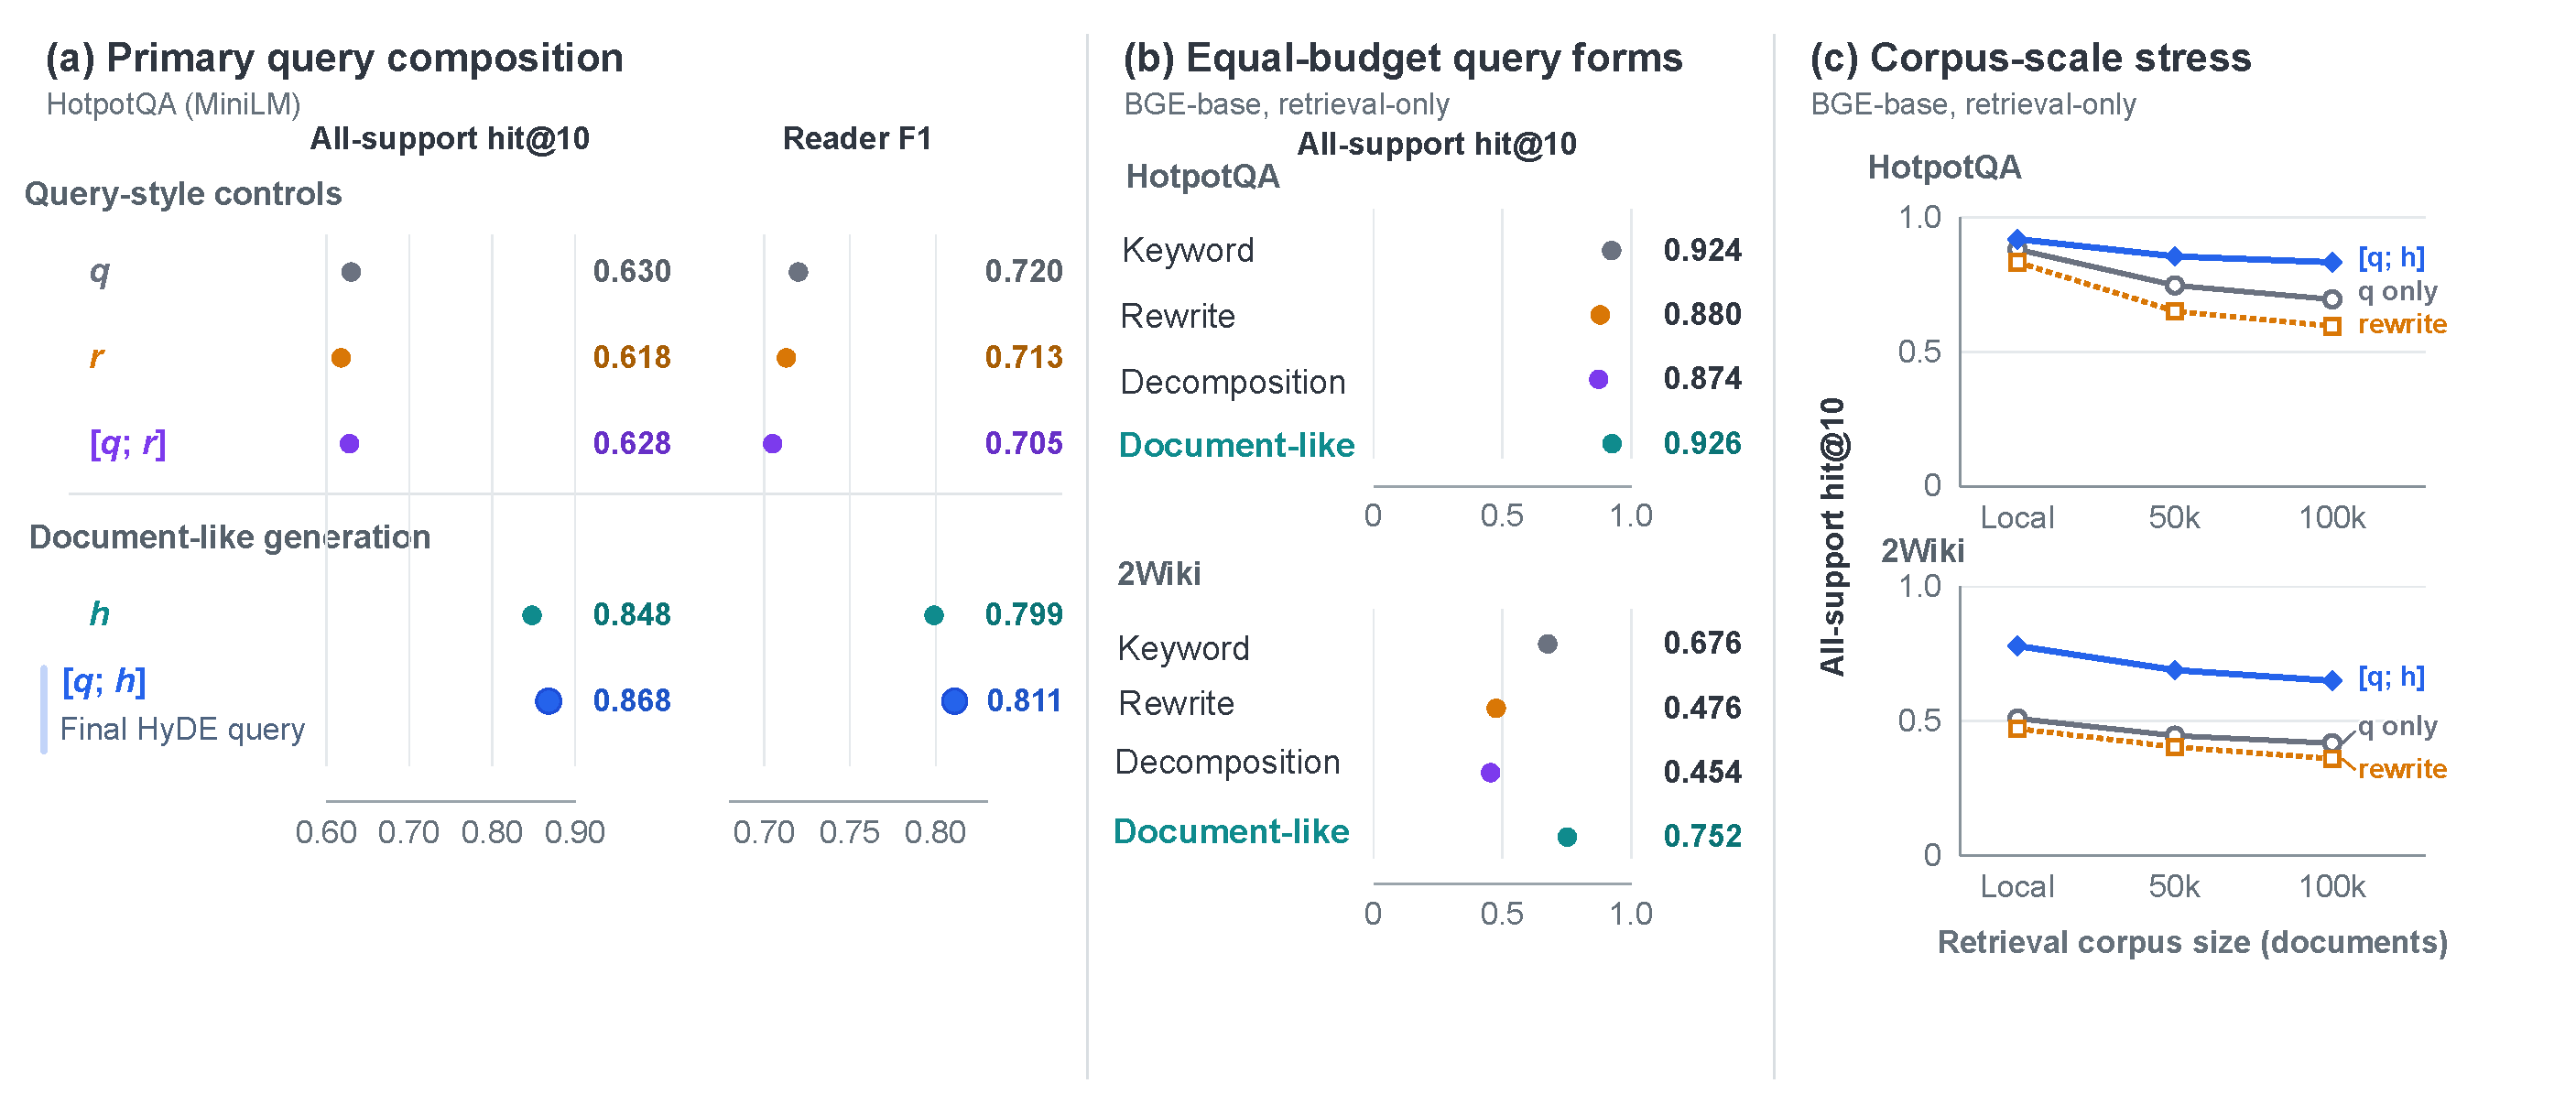
\includegraphics[width=\textwidth]{Fig2.pdf}
\caption{Empirical evidence for HyDE-style query construction. Panel (a) compares primary query compositions on HotpotQA using all-support hit@10 and reader F1. Panel (b) compares equal-budget query forms on HotpotQA and 2WikiMultihopQA. Panel (c) reports all-support hit@10 as the retrieval corpus expands from the original local corpus to 50k and 100k total documents by adding processed-train distractors. Here, $q$ denotes the original question, $r$ a rewritten query, and $h$ a document-like hypothetical passage; $[q; r]$ concatenates the question and rewrite, and $[q; h]$ is the final HyDE query.}
\label{fig:hyde_mechanism_overlap}
\end{figure*}

% Compact main-paper tables for the HyDE-enhanced RAG manuscript.

\begin{table*}[t]
\centering
\caption{Main results on the released IRCoT HotpotQA \texttt{test\_subsampled} split.}
\label{tab:main_results}
\scriptsize
\begin{threeparttable}
\setlength{\tabcolsep}{3pt}
\begin{tabularx}{\textwidth}{>{\raggedright\arraybackslash}X r r r r r}
\toprule
Method & Any hit@10 & All hit@10 & Recall@10 & EM & F1 \\
\midrule
LLM-only / No Retrieval & -- & -- & -- & 0.5200 & 0.6658 \\
One-step Dense RAG & 0.9860 & 0.6300 & 0.8080 & 0.5940 & 0.7199 \\
Multi-query RAG & 0.9860 & 0.6300 & 0.8080 & 0.5860 & 0.7028 \\
Single-query Reformulation RAG & 0.9800 & 0.6180 & 0.7990 & 0.5960 & 0.7130 \\
BM25 RAG & 0.9860 & 0.7320 & 0.8590 & 0.6240 & 0.7436 \\
BM25 + Dense Hybrid & \best{0.9900} & 0.7480 & 0.8690 & 0.6400 & 0.7577 \\
Rule-based Evidence-Expanded Iterative Retrieval & 0.9860 & 0.7540 & 0.8700 & 0.6360 & 0.7565 \\
\rowcolor{gray!10} HyDE-style RAG & 0.9880 & \best{0.8680} & \best{0.9280} & \best{0.6840} & \best{0.8105} \\
\bottomrule
\end{tabularx}
\begin{tablenotes}
\footnotesize
\item All rows use 500 HotpotQA examples and the same evidence-grounded Qwen3.7-Max reader. Retrieval rows use top-$k=10$ under the processed local-corpus protocol; the LLM-only row has no retrieval. Dense, BM25, and Hybrid are implemented lightweight baselines; Single-query Reformulation is a matched-call mechanism control; Multi-query and Rule-based Evidence-Expanded Iterative Retrieval are fixed heuristic controls. The primary comparisons are HyDE-style RAG against one-step Dense RAG and Single-query Reformulation. Bold marks column maxima, and shading marks the primary HyDE-style method.
\end{tablenotes}
\end{threeparttable}
\end{table*}

\begin{table*}[t]
\centering
\caption{HyDE query-composition diagnostic on the released IRCoT HotpotQA \texttt{test\_subsampled} split.}
\label{tab:hyde_query_ablation}
\small
\begin{threeparttable}
\begin{tabularx}{\textwidth}{>{\raggedright\arraybackslash}X r r r r r}
\toprule
Query used for dense retrieval & Any hit@10 & All hit@10 & Recall@10 & EM & F1 \\
\midrule
Question only & 0.9860 & 0.6300 & 0.8080 & 0.5940 & 0.7199 \\
Single rewritten query & 0.9800 & 0.6180 & 0.7990 & 0.5960 & 0.7130 \\
Question + rewritten query & 0.9780 & 0.6280 & 0.8030 & 0.5800 & 0.7048 \\
Hypothetical passage only & \best{0.9880} & 0.8480 & 0.9180 & 0.6780 & 0.7986 \\
Question + hypothetical passage & \best{0.9880} & \best{0.8680} & \best{0.9280} & \best{0.6840} & \best{0.8105} \\
\bottomrule
\end{tabularx}
\begin{tablenotes}
\footnotesize
\item All rows share the MiniLM index, top-$k=10$, query serialization, tokenization and truncation policy, and evidence-grounded Qwen3.7-Max reader. Question only reproduces the dense baseline. Single rewritten query and question + rewritten query are matched-call controls for direct reformulation and retained question text. Hypothetical passage only and question + hypothetical passage test document-like generation and query composition. The reader receives only retrieved corpus passages; the exact encoder configuration is reported in Online Resource 1, Section~\SuppRef{sec:supp_dense_encoder_truncation}.
\end{tablenotes}
\end{threeparttable}
\end{table*}


\FloatBarrier
\section{MultiHop-RAG Available-Condition External Validation}
\label{sec:supp_mhrag_external}

This section reports the completed available-condition matrix and the separate S3 retrieval robustness study. It does not certify completion of the full registered six-condition family or independent human validation. Framework, claim-stress and supporting-sentence audits are completed in Sections S21--S22; the planned human component was withdrawn under the scope amendment below. IRCoT's frozen local adapter is technically ineligible for this corpus; no failed or missing run is assigned a numerical score. Four observed method-versus-BM25 contrasts retain a conservative fifth multiplicity slot at 1.0. The primary endpoints are non-null all-support retrieval and answer EM; F1 and null abstention are secondary. All paired intervals resample questions 10,000 times with seed 13; binary main effects use exact McNemar tests, while reader interactions use paired sign-flip inference.

The official release is pinned to revision \path{71ac0d0bd1f951d2d6b70311f7d2ae404e1ffa82}. The source has 2,556 fixed ordered questions, including 301 null queries. The BGE checkpoint revision is \path{a5beb1e3e68b9ab74eb54cfd186867f64f240e1a}; the cross-encoder revision is \path{953dc6f6f85a1b2dbfca4c34a2796e7dde08d41e}. Parent evidence IDs define retrieval support. The frozen standard HyDE condition uses the question plus generated text, top-10 retrieval, greedy generation and the original prompt; hypothetical text is never reader evidence. The two revision-pinned readers retain the 450/900 character serializers, 2,000-token input budget, greedy seed 13 and 32-token output limit. The corrected serializer preserves the complete answer/chat suffix by budgeting evidence first. Five Qwen/450 cells have independently verified effective-token identity with the historical sealed source; all other cells belong to the new corrected execution namespace. The invalid historical Qwen/900 prefix is neither used nor overwritten.

The answer seal binds 20 cells and 51,120 rows, including unique ordered IDs, recomputed scores, frozen parameters, actual effective-input hashes, EOS/output-cap termination and independent archive copies. The S3 seal binds 12 generation and 12 retrieval cells, each totaling 4,800 rows. The table reconstruction manifest is \path{artifacts/tables/jiis_chatfix_available_v2/manifest.json}; it binds all consumed summary hashes, both independent seals, the builder and generated tables. Its release-readiness and full-family flags are false. Complete paired EM/F1, abstention and secondary cost comparisons remain in \path{artifacts/summaries/jiis_acceptance_v3/reader_chatfix_v1/answers/paired_comparisons.csv}; reader interactions and cost summaries are separately hash-bound. Licensed/private text and the coordinator-only blind allocation key are outside these tables.

% Generated by scripts/build_jiis_chatfix_tables.py; available evidence only.
\begin{table*}[!htbp]
\centering\footnotesize
\caption{MultiHop-RAG answer outcomes with both frozen evidence lengths.}
\label{tab:mhrag_answers}
\begin{threeparttable}
\setlength{\tabcolsep}{3pt}
\begin{tabular}{llrrrr}
\toprule
Chars & Method & Qwen EM & Qwen F1 & Mistral EM & Mistral F1 \\
\midrule
450 & BM25 & 0.316 & 0.321 & 0.249 & 0.306 \\
450 & Dense BGE & 0.319 & 0.325 & 0.262 & 0.309 \\
450 & Qwen-HyDE & 0.295 & 0.299 & 0.238 & 0.283 \\
450 & Mistral-HyDE & 0.286 & 0.291 & 0.242 & 0.289 \\
450 & Cross-encoder & 0.329 & 0.334 & 0.265 & 0.315 \\
900 & BM25 & 0.318 & 0.326 & 0.231 & 0.289 \\
900 & Dense BGE & 0.324 & 0.328 & 0.253 & 0.299 \\
900 & Qwen-HyDE & 0.290 & 0.294 & 0.219 & 0.264 \\
900 & Mistral-HyDE & 0.287 & 0.293 & 0.217 & 0.265 \\
900 & Cross-encoder & 0.336 & 0.342 & 0.240 & 0.292 \\
\bottomrule
\end{tabular}
\begin{tablenotes}\scriptsize\item Each cell includes 2,556 outputs: EM/F1 use 2,255 non-null questions; null-query abstention is reported separately. These are deterministically adapted scores. Both lengths are retained without selecting a best setting. Corrected evidence budgeting preserves the full chat suffix within 2,000 input tokens; the output limit is 32 tokens. The five Qwen/450 cells are explicitly token-identical historical reuse. Paired EM decisions and raw-score decomposition are in the supplementary external-validation section.
\end{tablenotes}
\end{threeparttable}
\end{table*}

% Generated by scripts/build_jiis_chatfix_tables.py; available evidence only.
\begin{table*}[!htbp]
\centering\footnotesize
\caption{Paired primary answer EM contrasts versus BM25.}
\label{tab:mhrag_em}
\begin{threeparttable}
\setlength{\tabcolsep}{3pt}
\begin{tabular}{lllrllr}
\toprule
Reader & Chars & Target & $\Delta$EM & 95\% CI & $p_{\rm Holm}$ & Direction \\
\midrule
Qwen & 450 & Dense BGE & +0.004 & [-0.006, +0.013] & 1.000 & unresolved \\
Qwen & 450 & Qwen-HyDE & -0.021 & [-0.031, -0.010] & $<0.001$ & negative \\
Qwen & 450 & Mistral-HyDE & -0.030 & [-0.041, -0.018] & $<0.001$ & negative \\
Qwen & 450 & Cross-encoder & +0.013 & [+0.004, +0.021] & 0.011 & positive \\
Mistral & 450 & Dense BGE & +0.012 & [+0.000, +0.024] & 0.204 & unresolved \\
Mistral & 450 & Qwen-HyDE & -0.012 & [-0.024, +0.001] & 0.279 & unresolved \\
Mistral & 450 & Mistral-HyDE & -0.008 & [-0.020, +0.005] & 0.550 & unresolved \\
Mistral & 450 & Cross-encoder & +0.016 & [+0.005, +0.027] & 0.031 & positive \\
Qwen & 900 & Dense BGE & +0.005 & [-0.005, +0.016] & 0.719 & unresolved \\
Qwen & 900 & Qwen-HyDE & -0.028 & [-0.040, -0.017] & $<0.001$ & negative \\
Qwen & 900 & Mistral-HyDE & -0.031 & [-0.043, -0.019] & $<0.001$ & negative \\
Qwen & 900 & Cross-encoder & +0.018 & [+0.009, +0.027] & $<0.001$ & positive \\
Mistral & 900 & Dense BGE & +0.022 & [+0.009, +0.034] & 0.005 & positive \\
Mistral & 900 & Qwen-HyDE & -0.012 & [-0.026, +0.000] & 0.236 & unresolved \\
Mistral & 900 & Mistral-HyDE & -0.014 & [-0.027, -0.001] & 0.200 & unresolved \\
Mistral & 900 & Cross-encoder & +0.009 & [-0.002, +0.020] & 0.256 & unresolved \\
\bottomrule
\end{tabular}
\begin{tablenotes}\scriptsize\item All-support and EM are primary endpoints. Four observed contrasts versus BM25 use Holm correction with a fifth slot conservatively reserved at 1.0 for unavailable IRCoT; this is not an observed IRCoT $p$-value. The full registered family is incomplete. Intervals are 95\% question-level bootstrap intervals (10,000 resamples); intervals alone do not determine significance. A positive or negative label denotes an adjusted within-configuration effect, not a complete transport decision.
\end{tablenotes}
\end{threeparttable}
\end{table*}

% Generated by scripts/build_jiis_chatfix_tables.py; available evidence only.
\begin{table*}[!htbp]
\centering\footnotesize
\caption{Raw/adapted answer scores and null-query abstention.}
\label{tab:mhrag_raw_null}
\begin{threeparttable}
\setlength{\tabcolsep}{3pt}
\begin{tabular}{lllrrrrrr}
\toprule
Reader & Chars & Method & Raw EM & EM & Raw F1 & F1 & Raw null & Null \\
\midrule
Qwen & 450 & BM25 & 0.316 & 0.316 & 0.321 & 0.321 & 0.724 & 0.724 \\
Qwen & 450 & Dense BGE & 0.319 & 0.319 & 0.325 & 0.325 & 0.654 & 0.654 \\
Qwen & 450 & Qwen-HyDE & 0.295 & 0.295 & 0.299 & 0.299 & 0.741 & 0.741 \\
Qwen & 450 & Mistral-HyDE & 0.286 & 0.286 & 0.291 & 0.291 & 0.701 & 0.701 \\
Qwen & 450 & Cross-encoder & 0.329 & 0.329 & 0.334 & 0.334 & 0.641 & 0.641 \\
Qwen & 900 & BM25 & 0.318 & 0.318 & 0.326 & 0.326 & 0.661 & 0.661 \\
Qwen & 900 & Dense BGE & 0.324 & 0.324 & 0.328 & 0.328 & 0.631 & 0.631 \\
Qwen & 900 & Qwen-HyDE & 0.290 & 0.290 & 0.294 & 0.294 & 0.714 & 0.714 \\
Qwen & 900 & Mistral-HyDE & 0.287 & 0.287 & 0.293 & 0.293 & 0.721 & 0.721 \\
Qwen & 900 & Cross-encoder & 0.336 & 0.336 & 0.342 & 0.342 & 0.621 & 0.621 \\
Mistral & 450 & BM25 & 0.249 & 0.249 & 0.306 & 0.306 & 0.113 & 0.113 \\
Mistral & 450 & Dense BGE & 0.260 & 0.262 & 0.308 & 0.309 & 0.120 & 0.120 \\
Mistral & 450 & Qwen-HyDE & 0.237 & 0.238 & 0.282 & 0.283 & 0.150 & 0.150 \\
Mistral & 450 & Mistral-HyDE & 0.241 & 0.242 & 0.288 & 0.289 & 0.153 & 0.153 \\
Mistral & 450 & Cross-encoder & 0.265 & 0.265 & 0.315 & 0.315 & 0.123 & 0.123 \\
Mistral & 900 & BM25 & 0.230 & 0.231 & 0.288 & 0.289 & 0.030 & 0.030 \\
Mistral & 900 & Dense BGE & 0.251 & 0.253 & 0.298 & 0.299 & 0.047 & 0.047 \\
Mistral & 900 & Qwen-HyDE & 0.218 & 0.219 & 0.264 & 0.264 & 0.053 & 0.053 \\
Mistral & 900 & Mistral-HyDE & 0.215 & 0.217 & 0.263 & 0.265 & 0.066 & 0.066 \\
Mistral & 900 & Cross-encoder & 0.240 & 0.240 & 0.292 & 0.292 & 0.030 & 0.030 \\
\bottomrule
\end{tabular}
\begin{tablenotes}\scriptsize\item EM/F1 denominator: 2,255; null denominator: 301. Null measures canonical abstention correctness, not support retrieval. Raw scores retain model formatting; adapted scores use the fixed adapter. No manual labels enter these metrics.
\end{tablenotes}
\end{threeparttable}
\end{table*}

% Generated by scripts/build_jiis_chatfix_tables.py; available evidence only.
\begin{table*}[!htbp]
\centering\footnotesize
\caption{Exploratory Qwen-minus-Mistral EM-effect interactions.}
\label{tab:mhrag_interactions}
\begin{threeparttable}
\setlength{\tabcolsep}{3pt}
\begin{tabular}{llrlr}
\toprule
Chars & Target versus BM25 & Interaction & 95\% CI & $p_{\rm Holm}$ \\
\midrule
450 & Dense BGE & -0.009 & [-0.023, +0.005] & 0.999 \\
450 & Qwen-HyDE & -0.009 & [-0.025, +0.007] & 0.999 \\
450 & Mistral-HyDE & -0.022 & [-0.038, -0.007] & 0.035 \\
450 & Cross-encoder & -0.003 & [-0.017, +0.010] & 1.000 \\
900 & Dense BGE & -0.016 & [-0.032, -0.001] & 0.174 \\
900 & Qwen-HyDE & -0.016 & [-0.031, -0.000] & 0.174 \\
900 & Mistral-HyDE & -0.017 & [-0.033, -0.001] & 0.166 \\
900 & Cross-encoder & +0.008 & [-0.005, +0.022] & 0.491 \\
\bottomrule
\end{tabular}
\begin{tablenotes}\scriptsize\item Interaction is (target minus BM25) for Qwen minus the same effect for Mistral. Question-paired sign-flip inference uses 10,000 draws and the conservative five-slot family. Non-significance does not demonstrate reader invariance.
\end{tablenotes}
\end{threeparttable}
\end{table*}

\FloatBarrier

The prompt subset contains 500 non-null questions, and the seed subset contains 300 different non-null questions. Prompt conditions are greedy standard, evidence-only and query2doc-style; the two target-versus-standard contrasts are Holm-corrected within each generator/endpoint. The seed study uses the standard prompt with temperature 0.7 at seeds 13, 37 and 101. All generation caps are 96 tokens. Question-level bootstrap preserves the three seed outcomes together. No alternative prompt or seed is promoted into the primary answer matrix, and no answer experiment has been performed for these S3 alternatives.

% Generated by scripts/build_jiis_chatfix_tables.py; available evidence only.
\begin{table*}[!htbp]
\centering\footnotesize
\caption{Prompt sensitivity on the fixed 500-question subset.}
\label{tab:mhrag_prompts}
\begin{threeparttable}
\setlength{\tabcolsep}{3pt}
\begin{tabular}{llrrrlr}
\toprule
Generator & Target & Standard & Target All & $\Delta$All & 95\% CI & $p_{\rm Holm}$ \\
\midrule
Qwen & evidence-only & 0.458 & 0.488 & +0.030 & [+0.002, +0.058] & 0.053 \\
Qwen & query2doc & 0.458 & 0.516 & +0.058 & [+0.030, +0.086] & $<0.001$ \\
Mistral & evidence-only & 0.454 & 0.454 & +0.000 & [-0.030, +0.030] & 1.000 \\
Mistral & query2doc & 0.454 & 0.512 & +0.058 & [+0.024, +0.092] & 0.003 \\
\bottomrule
\end{tabular}
\begin{tablenotes}\scriptsize\item Two contrasts versus standard are Holm-corrected separately within each generator and endpoint. Greedy decoding uses seed 13 and a 96-token cap. The query2doc-style prompt is a controlled adaptation. This subset does not establish superiority over question-only Dense or an answer improvement; no prompt replaces the primary standard condition.
\end{tablenotes}
\end{threeparttable}
\end{table*}

% Generated by scripts/build_jiis_chatfix_tables.py; available evidence only.
\begin{table*}[!htbp]
\centering\footnotesize
\caption{Descriptive seed sensitivity on the separate 300-question subset.}
\label{tab:mhrag_seeds}
\begin{threeparttable}
\setlength{\tabcolsep}{3pt}
\begin{tabular}{lrrrrrl}
\toprule
Generator & Seed 13 & Seed 37 & Seed 101 & Mean & SD means & 95\% CI mean \\
\midrule
Qwen & 0.517 & 0.507 & 0.520 & 0.514 & 0.007 & [0.461, 0.569] \\
Mistral & 0.483 & 0.453 & 0.473 & 0.470 & 0.015 & [0.417, 0.524] \\
\bottomrule
\end{tabular}
\begin{tablenotes}\scriptsize\item All-support@10; standard prompt, sampling temperature 0.7, 96-token cap. SD is the sample SD of three seed means. Intervals resample questions jointly across seeds; seeds are not independent replicates. No best-seed selection or invariance test is made.
\end{tablenotes}
\end{threeparttable}
\end{table*}

\FloatBarrier
% Generated by scripts/build_jiis_chatfix_tables.py; available evidence only.
\begin{table*}[!htbp]
\centering\footnotesize
\caption{Observed reader-call cost, not end-to-end system cost.}
\label{tab:mhrag_cost}
\begin{threeparttable}
\setlength{\tabcolsep}{3pt}
\begin{tabular}{lllrrrr}
\toprule
Reader & Chars & Method & Mean s & P95 s & Input tokens & Output tokens \\
\midrule
Qwen & 450 & BM25 & 1.50 & 1.37 & 1347.0 & 2.67 \\
Qwen & 450 & Dense BGE & 1.24 & 1.41 & 1332.2 & 2.67 \\
Qwen & 450 & Qwen-HyDE & 1.21 & 1.40 & 1319.2 & 2.63 \\
Qwen & 450 & Mistral-HyDE & 1.20 & 1.38 & 1319.8 & 2.65 \\
Qwen & 450 & Cross-encoder & 1.29 & 1.45 & 1358.3 & 2.68 \\
Qwen & 900 & BM25 & 2.13 & 3.27 & 1999.8 & 2.66 \\
Qwen & 900 & Dense BGE & 1.87 & 2.04 & 1993.5 & 2.69 \\
Qwen & 900 & Qwen-HyDE & 1.86 & 2.02 & 1995.3 & 2.67 \\
Qwen & 900 & Mistral-HyDE & 1.85 & 2.02 & 1994.2 & 2.65 \\
Qwen & 900 & Cross-encoder & 1.86 & 2.02 & 1999.8 & 2.70 \\
Mistral & 450 & BM25 & 2.81 & 3.40 & 1444.0 & 13.77 \\
Mistral & 450 & Dense BGE & 2.04 & 2.92 & 1427.7 & 13.08 \\
Mistral & 450 & Qwen-HyDE & 2.23 & 3.08 & 1409.9 & 12.89 \\
Mistral & 450 & Mistral-HyDE & 2.37 & 3.05 & 1410.8 & 13.02 \\
Mistral & 450 & Cross-encoder & 2.51 & 3.55 & 1456.0 & 13.21 \\
Mistral & 900 & BM25 & 5.42 & 10.17 & 2000.0 & 18.38 \\
Mistral & 900 & Dense BGE & 7.83 & 13.88 & 1998.8 & 17.17 \\
Mistral & 900 & Qwen-HyDE & 8.33 & 14.04 & 1999.7 & 17.65 \\
Mistral & 900 & Mistral-HyDE & 8.29 & 14.31 & 1999.5 & 17.49 \\
Mistral & 900 & Cross-encoder & 7.86 & 15.46 & 2000.0 & 17.81 \\
\bottomrule
\end{tabular}
\begin{tablenotes}\scriptsize\item Means cover 2,556 queries per cell. Times include successful reading/adaptation only and differ by runtime cohort; historical Qwen/450 uses a shared worker, other cells fresh workers. Input lengths for historical reuse are reconstructed token-identically. Missing: failed-attempt/load/queue durations, historical peak memory, exact HyDE-generator emitted token counts, per-query dense timing and end-to-end latency. No dollar estimate or algorithmic speedup is inferred. Per query, HyDE adds one generation and one dense search; Dense uses one dense search; cross-encoder uses one BM25 search and 100 pair scores; BM25 uses one search. All methods use one reader call, plus recorded retries if present.
\end{tablenotes}
\end{threeparttable}
\end{table*}


A retrospective scope amendment dated 2026-10-03 withdrew the planned 120-item independent human audit because qualified annotators could not be recruited. The amendment occurred after automated results were available, but no labels were collected; no annotation outcome informed the decision. Original plans, the packet and blank forms remain archived. The raw/adapted answer analysis is retained. No replacement LLM judge or human agreement statistic is introduced. Benchmark-based scores and official-sentence retention remain automated diagnostics, while the older single-annotator taxonomy remains illustrative. Independent human evidence sufficiency and error-category reliability were not evaluated. The versioned amendment and preserved-source hashes are recorded in \path{docs/experiments/jiis_human_audit_scope_amendment_2026-10-03.json}; original absence and release-readiness flags are not rewritten.
\FloatBarrier



\section{Reporting-rule Stress Test and Framework Positioning}
\label{sec:supp_claim_stress}
The S4 registry comprises the 12 unique primary effects in the canonical S1 boundary matrix and all 20 observed S2 retrieval/EM contrasts. Repeated source effects are counted once; secondary serializer, F1, raw-output and prompt/seed measures are excluded. The existing family-specific adjusted values are reused, including the reserved IRCoT slots. Five unobserved IRCoT primary comparisons are reported as missing, not fabricated measurements. The stress test is descriptive and cannot establish the accuracy of a reporting strategy. Local effect decisions are distinct from the source-and-required-target transfer rule. The full ten-dimension source-backed comparison is in \texttt{docs/literature/rag\_evaluation\_framework\_comparison.tsv}; the comparison is interpretive positioning, not an empirical execution of the three tools. ARES (Saad-Falcon et al., 2024) supplies PPI uncertainty, RAGAS (Es et al., 2024) quality metrics, and RAGChecker (Ru et al., 2024) claim-level diagnostics.
% Generated by scripts/build_jiis_chatfix_tables.py; available evidence only.
\begin{table*}[!htbp]
\centering\footnotesize
\caption{Descriptive claim-stress analysis of 32 unique observed primary effects.}
\label{tab:claim_stress}
\begin{threeparttable}
\setlength{\tabcolsep}{3pt}
\begin{tabular}{lrrrr}
\toprule
Reporting rule & Favorable & Adverse & Unresolved & $n$ \\
\midrule
point only & 19 & 13 & 0 & 32 \\
interval only & 15 & 10 & 7 & 32 \\
unadjusted test & 13 & 9 & 10 & 32 \\
adjusted audit & 12 & 7 & 13 & 32 \\
\bottomrule
\end{tabular}
\begin{tablenotes}\scriptsize\item Counts reuse frozen S1/S2 effects and their original corrections. Point/interval labels are hypothetical reporting decisions, not new evidence. Five unavailable IRCoT slots are excluded from observed counts and remain missing. Local edge decisions differ from aggregate transfer decisions.
\end{tablenotes}
\end{threeparttable}
\end{table*}

% Generated by scripts/build_jiis_chatfix_tables.py; available evidence only.
\begin{table*}[!htbp]
\centering\footnotesize
\caption{Framework positioning from primary papers; no empirical tool comparison.}
\label{tab:framework_comparison}
\begin{threeparttable}
\setlength{\tabcolsep}{3pt}
\begin{tabular}{p{.16\textwidth}p{.30\textwidth}p{.42\textwidth}}
\toprule
Framework & Unit & Output \\
\midrule
RAGAS & Question, response and retrieved context & Faithfulness and relevance scores \\
ARES & System quality from trained judges & Quality estimates and PPI confidence intervals \\
RAGChecker & Claims, retrieved chunks and responses & Overall and component diagnostic scores \\
reliability boundary audit & Question-paired configuration effects & Supported, rejected or unresolved within specified scope \\
\bottomrule
\end{tabular}
\begin{tablenotes}\scriptsize\item RAGAS: Es et al. (2024), sec. 3; ARES: Saad-Falcon et al. (2024), sec. 3; RAGChecker: Ru et al. (2024), sec. 3 and appendix A. The full source-backed TSV compares ten dimensions. ARES includes PPI uncertainty; these approaches answer complementary questions.
\end{tablenotes}
\end{threeparttable}
\end{table*}

The write-once task8 contract, 32-row registry, summaries and output hashes are in \texttt{artifacts/summaries/jiis\_acceptance\_v3/task8\_task9\_v1/}. No generation settings or underlying scores were changed. The verified S1 corpus-scale contrast has adjusted $p=2.22825910896\times10^{-5}$, while both 2Wiki answer contrasts remain unresolved.


\section{Official Supporting-sentence Audit}
\label{sec:supp_sentence_audit}
This S5 diagnostic freezes the existing 500 HotpotQA IDs and the four original retrieval files (OneR, HyDE, IRCoT, BGE-base rescore). It does not rerun retrieval or add the learned cross-encoder to this registered audit. After the original CMU download failed, the dev-distractor sentence arrays and facts were acquired from the HotpotQA-hosted Hugging Face conversion at revision \texttt{1908d6afbbead072334abe2965f91bd2709910ab}. The parquet source, structure-only JSON conversion and acquisition manifest are separately hashed. This is retrospective source acquisition, not a byte-identical download of the original CMU JSON or an original pre-experiment source freeze.

All 500 question strings and all previously annotated supporting paragraphs match after the existing whitespace normalization. One question (\texttt{5a79c7ac5542994bb9457097}) uses \emph{Counting On} in official facts and \emph{List of Counting On episodes} in the frozen paragraph labels. Official-sentence metrics and the original frozen-label metrics are therefore recorded separately without changing any primary retrieval score or dropping a question. The original eight method/budget paragraph summaries are independently reproduced. The complete source contains one invalid fact index outside the frozen sample; none of the 500 selected fact indices is invalid. Two selected unannotated empty sentence positions are preserved, without renumbering official facts.

The 4,000-row audit maps official indexed sentence ends onto the actual retrieved paragraph's character offsets after an exact whitespace-normalized paragraph match. The serializer is \texttt{str(text).strip()[:budget]} at 450 or 900 characters, before any separate model input-token budget. These are per-document character-interface diagnostics, not full chat-token retention measurements. Supporting-title completeness, exact paragraph matching, complete-paragraph retention and all-annotated-sentence retention are computed independently. Answer-string presence is only a normalized substring diagnostic, including yes/no strings; it is never substituted for annotated support. The question set is never reduced based on outcomes. No supervision is added to retrieval or generation inputs.
% Generated by scripts/build_jiis_chatfix_tables.py; available evidence only.
\begin{table*}[!htbp]
\centering\footnotesize
\caption{Official supporting-sentence retention on the same 500 HotpotQA questions.}
\label{tab:supporting_sentence_audit}
\begin{threeparttable}
\setlength{\tabcolsep}{3pt}
\begin{tabular}{lrrrrr}
\toprule
Method & Chars & Titles & Full para. & Support sent. & Answer string \\
\midrule
one & 450 & 0.298 & 0.112 & 0.254 & 0.478 \\
one & 900 & 0.298 & 0.288 & 0.298 & 0.506 \\
hyde & 450 & 0.350 & 0.102 & 0.284 & 0.538 \\
hyde & 900 & 0.350 & 0.334 & 0.350 & 0.568 \\
ircot & 450 & 0.354 & 0.140 & 0.298 & 0.536 \\
ircot & 900 & 0.354 & 0.340 & 0.354 & 0.552 \\
rescore & 450 & 0.462 & 0.176 & 0.388 & 0.586 \\
rescore & 900 & 0.462 & 0.436 & 0.462 & 0.614 \\
\bottomrule
\end{tabular}
\begin{tablenotes}\scriptsize\item Official sentence IDs come from the pinned HotpotQA-hosted dev-distractor conversion. All 500 questions align; one official supporting-title set differs from the frozen labels. This table uses official facts; the original-label audit is separately reconstructed without changing scores or omitting a question. Prefix serialization uses actual character offsets. Answer-string presence is a separate substring diagnostic, not factual sufficiency or human agreement.
\end{tablenotes}
\end{threeparttable}
\end{table*}

At 450 characters, sentence retention exceeds complete-paragraph retention for every tested method; at 900 characters, all retrieved official annotated support survives in this sample. This bounds the earlier conservative paragraph-loss interpretation, without proving that retained sentences suffice to answer a question. The sentence-v3 contract, eight summary cells and hashes are in \texttt{artifacts/summaries/jiis\_acceptance\_v3/task8\_task9\_v1/sentence\_v3/}. The earlier sentence-v2 contract and failed checks remain diagnostic evidence. The planned Task 10 human component was withdrawn under the disclosed scope amendment; human evidence-sufficiency labels and inter-annotator agreement are still absent.

\FloatBarrier
\section{Post-hoc Matched Comparisons, Final-input and Scorer Audits}
\label{sec:supp_priority_diagnostics}

These diagnostics were added after the original results were observed. They do not replace historical scores, frozen families or the withdrawn human audit. New source hashes, contracts and sanitized summaries are recorded under \path{artifacts/summaries/jiis_priority_revision_20261003/}. Private working inputs remain under a separate local directory. No generated answer was used to select the diagnostic subsets.

\subsection{Matched Dense and Prompt-subset Comparisons}
The analysis preserves exact ID order before separating 2,255 non-null news questions. It freezes three additional families containing six retrieval, 16 answer and 36 prompt-versus-baseline contrasts. Binary endpoints use two-sided exact McNemar tests; continuous F1/recall endpoints use Monte Carlo sign flips with the plus-one correction. Paired percentile intervals use 10,000 resamples and seed 13. The existing BM25 family, including its unavailable IRCoT slot, is unchanged. These additional comparisons are post hoc rather than retrospectively registered primary tests.

\begin{table*}[htbp]
\centering\footnotesize
\caption{Selected post-hoc news comparisons with the matched Dense baseline. Delta is target minus Dense. All rows use 2,255 non-null questions; adjusted tests belong to the new six-retrieval or 16-answer family.}
\label{tab:priority_dense_pairs}
\begin{tabularx}{\textwidth}{X l r r l r}
\toprule
Target & Endpoint & Reader & Chars & $\Delta$ [95\% CI] & $p_{\mathrm{Holm}}$ \\
\midrule
Qwen-HyDE & all-support & -- & -- & $-0.0550$ [$-0.0710,-0.0395$] & $2.29\times10^{-11}$ \\
Mistral-HyDE & all-support & -- & -- & $-0.0692$ [$-0.0851,-0.0537$] & $3.24\times10^{-17}$ \\
Qwen-HyDE & EM & Qwen & 450 & $-0.0244$ [$-0.0337,-0.0151$] & $2.42\times10^{-6}$ \\
Mistral-HyDE & EM & Qwen & 450 & $-0.0333$ [$-0.0430,-0.0239$] & $1.87\times10^{-10}$ \\
Qwen-HyDE & EM & Qwen & 900 & $-0.0337$ [$-0.0439,-0.0235$] & $5.34\times10^{-10}$ \\
Mistral-HyDE & EM & Qwen & 900 & $-0.0364$ [$-0.0470,-0.0266$] & $2.66\times10^{-11}$ \\
Qwen-HyDE & EM & Mistral & 450 & $-0.0239$ [$-0.0355,-0.0124$] & 0.0008 \\
Mistral-HyDE & EM & Mistral & 450 & $-0.0200$ [$-0.0310,-0.0089$] & 0.0009 \\
Qwen-HyDE & EM & Mistral & 900 & $-0.0341$ [$-0.0457,-0.0226$] & $1.04\times10^{-7}$ \\
Mistral-HyDE & EM & Mistral & 900 & $-0.0355$ [$-0.0479,-0.0231$] & $1.05\times10^{-7}$ \\
\bottomrule
\end{tabularx}
\end{table*}

The frozen 500-question prompt subset is sliced from the same Dense/BM25 files using its original IDs, rather than compared to full-release averages. Dense all-support is 0.502 and BM25 is 0.590. Query2doc-style Qwen/Mistral scores are 0.516/0.512. Their Dense deltas are $+0.014$ [$-0.014,0.044$] and $+0.010$ [$-0.020,0.040$], both adjusted $p=1$. Their BM25 deltas are $-0.074$ [$-0.116,-0.032$] and $-0.078$ [$-0.122,-0.034$], adjusted $p=0.0192/0.0139$. Superiority to standard prompting therefore does not establish superiority to either matched baseline. The 58-row CSV includes all secondary endpoints, discordant counts and raw/adjusted tests.

\FloatBarrier
\subsection{Actual Final-input Evidence}
The HotpotQA audit reconstructs pinned chat templates and token offsets for five retrieval methods and both readers on all 500 IDs. Actual 450-character prompts match all 5,000 stored prompt hashes; none exceeds 2,000 input tokens. The historical artifacts do not retain effective-token hashes, so reconstructed token sequences are not described as historically hash-verified. The four original methods retain all official support sentences for 0.254/0.284/0.298/0.388 of questions. Adding the cross-encoder gives 0.470 retrieval completeness and 0.390 after character and token serialization for each reader. Official sentence labels remain separate from the original paragraph-label metrics. The 900-character inputs are counterfactual interface diagnostics, not previously executed HotpotQA answers.

The news audit verifies all 51,120 historical effective-token hashes across 20 corrected cells. Parent-document identity survives independently of whether a complete gold fact span remains in the supplied chunk. Each of 6,084 gold fact strings maps to one original parent after whitespace normalization. Only 583 are extractively present in the cross-encoder's retrieved chunk texts. All matching spans, rather than only a first occurrence, are checked through character offsets and final token offsets. Unmatched spans remain losses in the denominator. This exact-span diagnostic does not measure semantic equivalence, distributed evidence or human evidence sufficiency.

\begin{table*}[htbp]
\centering\footnotesize
\caption{News cross-encoder evidence reaching the actual reader input. Question rates use 2,255 non-null questions; counts use 6,084 gold fact entries. Parent survival means every required parent identity retains some body text, not its complete article. Matched facts require at least one complete exact span. Both budgets are actual executed news conditions.}
\label{tab:priority_news_token_retention}
\begin{tabularx}{\textwidth}{l r r r r r r}
\toprule
Reader & Chars & All-parent IDs & Final IDs & Chunk facts & Final facts & All-fact questions \\
\midrule
Qwen & 450 & 0.7286 & 0.7286 & 583 & 155 & 1/2255 \\
Mistral & 450 & 0.7286 & 0.7286 & 583 & 155 & 1/2255 \\
Qwen & 900 & 0.7286 & 0.6958 & 583 & 417 & 9/2255 \\
Mistral & 900 & 0.7286 & 0.6661 & 583 & 414 & 9/2255 \\
\bottomrule
\end{tabularx}
\end{table*}

At 900 characters, 423 fact spans survive character serialization before the final token budget removes six (Qwen) or nine (Mistral). Additional token-stage parent losses affect 74 and 141 non-null questions, respectively. Complete exact-span retention is 0.0004 at 450 characters and 0.0040 at 900 characters. These measurements explain why parent completeness cannot be interpreted as complete delivery of annotated facts. Descriptive associations with answer scores cannot identify a causal mediation effect.

\FloatBarrier
\subsection{Official Score-function Sensitivity}
The comparison uses official HotpotQA code at commit \texttt{3635853403a8735609ee997664e1528f4480762a} and 2Wiki v1.1 at \texttt{6bdd033bd51aae2d36ba939688c651b5c54ec28a}. Tests isolate punctuation/article order, categorical F1 and empty-answer behavior. Re-evaluation covers 20 available formal 500-row prediction files, retaining their existing adapted predictions and repository gold aliases. It excludes smoke files and pre-cost archive duplicates. This is a scalar score-function sensitivity check, not full official evaluation with a newly recovered 2Wiki alias/demonym dictionary or joint supporting-fact metrics.

EM remains unchanged in all audited files. Mean F1 decreases by 0.0033/0.0050/0.0045 for Mistral HotpotQA BM25/HyDE/IRCoT and 0.0054/0.0039 for BGE rescore/cross-encoder. Qwen HotpotQA HyDE and IRCoT decrease by 0.0005 each. Mistral 2Wiki BM25/HyDE/IRCoT/cross-encoder decrease by 0.0045/0.0040/0.0066/0.0032; other audited Qwen files are unchanged. Historical F1 contrasts and Holm families are preserved rather than silently relabeled as official metrics. Processed hosted raw answers were unavailable at their recorded local paths, preventing the same raw-prediction check for that tier.

\subsection{Canonical Abstention and Output Termination}
All 51,120 news rows reproduce their stored raw/adapted ordinary EM/F1 with zero mismatches. Null abstention is a separate endpoint over 301 questions, accepting only the registered canonical forms. A frozen lexical diagnostic additionally counts phrases expressing unknown or insufficient information, without awarding extra official credit. Raw/adapted predictions and 2,255 non-null questions are analyzed separately. Lexical matches can occur in mixed or explanatory responses and are not adjudicated semantic refusals.

For Mistral/900, BM25/cross-encoder canonical null accuracy is 0.0299/0.0299, while adapted lexical matches occur in 170/301 and 153/301 outputs. Qwen/900 canonical accuracy is 0.6611/0.6213. Newly generated rows expose exact emitted IDs and EOS/length termination; reused Qwen/450 rows lack those stop anchors. A token count of 32 is only a cap candidate when termination metadata is absent. No empty predictions were found. Mistral non-null length termination is approximately 17--19\% at 450 characters and 29--32\% at 900 characters. Strict canonical failures therefore combine possible answer errors, wording and formatting; they cannot be reported as a human-confirmed hallucination rate.

\FloatBarrier

\section{New Question-only and Gold-selected Reader Controls}
\label{sec:supp_reader_controls_new}
This diagnostic was frozen after historical outcomes were available but before its new answers. It uses the first 100 questions in the original 500-ID HotpotQA order, with no outcome-based selection. Qwen and Mistral each generate 100 question-only and 100 gold-support answers, following a separate two-question/two-condition smoke check. Protocols, model shard hashes, input-token hashes and receipts are preserved under \path{artifacts/summaries/jiis_priority_revision_20261003/reader_controls/} and its corresponding private local directory.

Gold-selected inputs contain every official supporting sentence and title, without inserting the answer field. All complete rendered inputs match their frozen tokens at inference, with no character clipping or token truncation. The prospectively allowed 8,192-token ceiling was unnecessary: maximum actual inputs are 298/314 tokens for Qwen/Mistral. Both readers use their pinned NF4 checkpoints, greedy seed 13 and at most 32 emitted tokens. Oracle evidence selection, instructions and evidence amount differ from retrieved-input conditions. This capability reference is neither a strict mathematical upper bound nor a causal retrieval-only ablation.

\begin{table*}[htbp]
\centering\footnotesize
\caption{Reader capability references and historical same-ID comparators on 100 HotpotQA questions. Means use adapted predictions. Official EM equals local EM here; F1 conventions remain separate. BM25 and cross-encoder answers are historical and are not regenerated.}
\label{tab:priority_reader_controls}
\begin{tabularx}{\textwidth}{l X r r r r}
\toprule
Reader & Evidence condition & $n$ & EM & Local F1 & Official F1 \\
\midrule
Qwen & Question only & 100 & 0.090 & 0.1407 & 0.1407 \\
Qwen & Gold-selected support & 100 & 0.570 & 0.6760 & 0.6760 \\
Qwen & BM25 & 100 & 0.180 & 0.2462 & 0.2462 \\
Qwen & Cross-encoder & 100 & 0.290 & 0.3752 & 0.3752 \\
\midrule
Mistral & Question only & 100 & 0.050 & 0.1950 & 0.1825 \\
Mistral & Gold-selected support & 100 & 0.350 & 0.5357 & 0.5267 \\
Mistral & BM25 & 100 & 0.150 & 0.2680 & 0.2643 \\
Mistral & Cross-encoder & 100 & 0.220 & 0.3685 & 0.3633 \\
\bottomrule
\end{tabularx}
\end{table*}

Four additional families (local/official EM/F1) each contain ten fixed contrasts, five per reader. EM uses exact two-sided McNemar; F1 uses explicitly Monte Carlo paired sign flips. Intervals use 10,000 paired bootstrap resamples and seed 13. Gold-minus-question-only EM is $+0.48$ [$0.38,0.58$] for Qwen and $+0.30$ [$0.21,0.39$] for Mistral, adjusted $p=9.06\times10^{-13}/1.23\times10^{-7}$. Gold-minus-cross-encoder EM is $+0.28$ [$0.18,0.38$] for Qwen, adjusted $p=1.36\times10^{-5}$. Mistral's $+0.13$ [$0.02,0.24$] remains unresolved ($p_{\mathrm{Holm}}=0.0702$), despite the interval excluding zero. Local and official EM families coincide for these data. Neither gold-selected condition yields perfect benchmark EM; that residual cannot be assigned uniquely to reasoning or formatting.

All 400 new raw/adapted predictions are re-evaluated against both scorers. Local metrics maximize over stored aliases; official metrics use the pinned HotpotQA scorer and its official single answer. Historical Qwen/BM25 lacks raw predictions, so its raw mean remains missing rather than substituted. Qwen emits EOS for all 200 answers with no cap hits. Mistral emits EOS for 174, with 27 cap hits (20 question-only, seven gold-support); one cap hit also ends with EOS. Actual cap and EOS indicators are therefore separate. Input/source hashes, score reconstruction and complete analysis rerun are verified.

\FloatBarrier

\section{New-sample Validation of Frozen Selection Rules}
\label{sec:supp_independent_validation_new}
This experiment freezes rules using historical outcomes, then evaluates new query outputs without changing those rules. It is prospective for the new outputs, not retrospective preregistration of the entire paper. The pinned HotpotQA dev source contains 7,405 questions. All old project result/prompt records identify 500 previously observed dev IDs; the first 64 remaining IDs in source order are selected. No new result, stratification or outcome screen determines membership. Sanitized metrics, overlap counts, contract hashes and completion records are in \path{artifacts/summaries/jiis_priority_revision_20261003/independent_validation/}; full inventories, contracts and private inputs remain in the corresponding local directory.

The retrieval-mean rule chooses among BM25, standard Qwen-HyDE/BM25 and the learned cross-encoder using old all-support means 0.298/0.348/0.468. The audit-informed rule uses their old equal-weight two-reader EM means 0.184/0.203/0.236. Ties resolve BM25, HyDE, then cross-encoder. Both rules choose the cross-encoder before new outcomes. Provenance, complete chat suffix and valid outputs are admissibility checks; they do not authorize changing the selected method or discarding unfavorable questions. This limited audit-informed rule does not operationalize every possible diagnostic or establish a general selection policy.

The restored index contains 5,233,329 records with no failed shards. CPU preparation performs 128 searches, top-10 and top-100 for each of 64 questions, taking 42.885 seconds. Cross-encoding scores 6,400 question--paragraph pairs and takes 490.991 successful-stage seconds, excluding 9.994 seconds of model loading. The pinned readers run sequentially on ten 450-character paragraph prefixes with greedy seed 13, 2,000 input tokens and 32 output tokens. Actual effective inputs and sentence offsets are frozen before reading and verified at runtime. There is no new HyDE generation or new BM25/HyDE reader outcome in this selected-policy experiment.

\begin{table*}[htbp]
\centering\footnotesize
\caption{Shared selected-policy results on 64 previously unobserved HotpotQA questions. Scores use the local full-wiki convention and fixed adapter. Both frozen rules select the same cross-encoder evidence; their performance difference is structural zero, without an inferential $p$-value.}
\label{tab:priority_independent_validation}
\begin{tabularx}{\textwidth}{l r r r r r r}
\toprule
Reader & $n$ & EM & F1 & Retrieved support & Final support & Length stops \\
\midrule
Qwen & 64 & 0.2813 & 0.3678 & 33/64 & 24/64 & 0/64 \\
Mistral & 64 & 0.2188 & 0.3706 & 33/64 & 24/64 & 6/64 \\
\bottomrule
\end{tabularx}
\end{table*}

All retrieved annotated support survives for 33/64 questions; 450-character serialization retains complete sentences for 24/64. Final token inputs retain the same 24/64, with no additional token truncation for either reader. Qwen emits EOS in all 64 outputs; Mistral has 58 EOS and six length stops. The fixed adapter changes nine Mistral texts and two score rows. All 128 reader calls, finite reranker scores, stable ordering, ID alignments, effective-input hashes and stored local scores pass verification.

Because the policies share the same method and outputs, $\Delta\mathrm{EM}=\Delta\mathrm{F1}=0$ by construction. No significance test is reported for identical policies. This is no observed decision increment, rather than evidence that the complete audit can never improve selection. The 64-question descriptive check neither measures unselected-method performance nor validates general routing accuracy. Stage timings belong to this execution cohort, exclude orchestration gaps and do not constitute a complete comparable end-to-end cost matrix.

\FloatBarrier

\section{Matched Character-budget Intervention}
\label{sec:supp_followup_serializer}

This same-question diagnostic was frozen after historical outcomes but before its new answers. It fixes the first 100 original HotpotQA IDs, saved cross-encoder top-10 paragraphs and both pinned NF4 readers. Each reader generates fresh 450- and 900-character conditions, with 2,000 input tokens, 32 output tokens, greedy decoding and seed 13: 400 formal answers after eight separate smoke answers. Historical 450-character predictions lack runtime token anchors and are not reused. Both new conditions use the same original full-wiki prompt and answer adapter, with the corrected evidence-tail policy preserving the complete answer/chat suffix. This is a matched interface-budget intervention, not independent validation, equal actual tokens or equal cost.

All 400 actual inputs match their frozen token IDs and contain the full suffix. No input reaches the token ceiling; maxima are 1,568 tokens for Qwen and 1,709 for Mistral. Strict whole-paragraph alignment and official sentence indices identify complete retrieved support in 55/100 questions. Increasing the character budget raises complete annotated-sentence retention from 46/100 to 55/100 for both readers, with no extra token-stage loss. These matches do not certify semantic sufficiency.

\begin{table*}[htbp]
\centering\footnotesize
\caption{Fresh matched serializer conditions on the same 100 questions. Scores use local adapted predictions; support is complete annotated-sentence retention in actual input. EOS and output-cap counts are measured separately from generated token IDs.}
\label{tab:followup_serializer_summary}
\begin{tabularx}{\textwidth}{l r r r r r r r}
\toprule
Reader & Chars & EM & F1 & Support & Mean input & EOS & Cap \\
\midrule
Qwen & 450 & 0.290 & 0.3752 & 46/100 & 965.92 & 100 & 0 \\
Qwen & 900 & 0.290 & 0.3890 & 55/100 & 1090.13 & 100 & 0 \\
Mistral & 450 & 0.220 & 0.3646 & 46/100 & 1054.94 & 93 & 7 \\
Mistral & 900 & 0.210 & 0.3780 & 55/100 & 1194.60 & 94 & 6 \\
\bottomrule
\end{tabularx}
\end{table*}

\begin{table*}[htbp]
\centering\footnotesize
\caption{Prospectively specified 900-minus-450 answer contrasts. Primary EM has a two-test exact McNemar/Holm family; secondary F1 has a separate two-test Monte Carlo sign-flip/Holm family. Intervals use 10,000 paired bootstrap resamples, seed 13, and are unadjusted. All four adjusted decisions are unresolved.}
\label{tab:followup_serializer_pairs}
\begin{tabularx}{\textwidth}{l l r l r r r}
\toprule
Reader & Endpoint & $\Delta$ & 95\% CI & Losses & Wins & $p_{\mathrm{Holm}}$ \\
\midrule
Qwen & EM & 0.0000 & $[-0.0500,0.0500]$ & 3 & 3 & 1.000 \\
Mistral & EM & $-0.0100$ & $[-0.0600,0.0300]$ & 3 & 2 & 1.000 \\
Qwen & F1 & 0.0138 & $[-0.0339,0.0648]$ & -- & -- & 1.000 \\
Mistral & F1 & 0.0134 & $[-0.0337,0.0610]$ & -- & -- & 1.000 \\
\bottomrule
\end{tabularx}
\end{table*}

The extra nine questions with retained complete support do not establish an EM or F1 gain. This result does not establish equivalence, nor identify the causal effect of semantic evidence sufficiency: evidence length and actual input tokens change together. Official single-answer EM agrees with local EM; Mistral official F1 is 0.3594/0.3719 at 450/900 characters, kept as descriptive scorer sensitivity. All 408 formal/smoke rows pass independent prompt reconstruction, effective-token, support, raw/adapted scoring, decoding and termination checks. A separate numeric-only reanalysis reproduces all four contrasts. Summaries, numeric provenance and sanitized score/support vectors are in \path{artifacts/summaries/jiis_followup_revision/serializer/}; private text remains excluded.

\FloatBarrier
\section{Complete Method Matrix on Random New Questions}
\label{sec:supp_followup_holdout}

This follow-up fixes a simple random sample of 300 questions from the same official HotpotQA development source. An inventory of 1,601 prior JSONL files identifies 564 previously observed IDs, including the original 500 and subsequent 64. One other question has an invalid official supporting-sentence index. The 6,840 eligible IDs are sorted, then sampled without replacement with Python Random(13), preserving draw order. No outcome-based exclusion, replacement or extension is permitted. New IDs do not establish a new dataset or absence of training contamination.

The scientific contract is frozen before new retrieval or model output. At question 136, a 200-hit raw window supplies only 86 unique CE candidates. An engineering amendment, frozen after 273 known CPU requests and before all model outputs, expands the raw window to 400 while retaining 100 unique candidates. Re-querying preserves all 135 completed top-100 lists byte-for-byte and in order. The amendment also enforces cumulative attempt accounting and exact ordered input/hash verification; it changes neither sample nor endpoints. Failed attempts and the earlier contract remain retained.

The three methods share the existing 5,233,329-paragraph index: question-only BM25, standard Qwen-HyDE/BM25 using question plus one hypothetical passage capped at 100 output tokens, and the pinned cross-encoder reranking BM25 top-100 to ten. Cross-encoder pairs use 512 tokens and float16; a synthetic throughput/memory benchmark fixes batch four before formal scores. Neither queries nor model inputs contain gold answers or support annotations. Both pinned readers use NF4, greedy seed 13, 450 characters per document, 2,000 input tokens and 32 output tokens. All six 300-row input cells are frozen before any reader answer, with the full answer/chat suffix preserved.

Primary local EM uses the single official answer and the existing answer adapter. Three method pairs under two readers form a six-test family; all-support-title retrieval has a separate three-test family. Secondary local F1 and official EM/F1 sensitivities each have separately labeled six-test families. Binary contrasts use exact McNemar; F1 uses 10,000 Monte Carlo paired sign flips with plus-one correction. Intervals use 10,000 paired bootstrap draws, seed 13, and are unadjusted. Holm correction is within each frozen family. At n=300, assumed five-percentage-point effects have only 20.4/8.6/5.6\% conservative power under discordance .2/.4/.6 and $\alpha=.05/6$; these pre-output assumptions are not measured power. The four-hour cumulative GPU ceiling includes loading, benchmarks, failures and resumed attempts. All results remain separate from historical 500-question means.

All 300 hypothetical passages, 30,000 formal CE pairs and 1,800 reader answers are complete. Independent reconstruction validates ordered IDs, the 135-row earlier CPU lineage, all six prompts/effective-token files, stable finite CE rankings, HyDE query composition, raw/adapted local and official scoring, and decoding/EOS/cap records. Strict complete annotated support is retrieved in 105/132/161 questions under BM25/HyDE/CE; character serialization retains 86/103/121, identical under both readers. There is no additional token-stage loss, with input maxima 1,399/1,523 tokens. These are exact-match support diagnostics, not human sufficiency labels.

\begin{table}[htbp]
\centering\footnotesize
\setlength{\tabcolsep}{3pt}
\renewcommand{\arraystretch}{1.08}
\caption{Random 300-question method matrix. All three methods are run under both readers; scores are local adapted answers. Retrieval is all-support-title hit@10. Complete support in input is strict annotated-sentence retention, identical across readers.}
\label{tab:followup_holdout_summary}
\begin{tabularx}{\textwidth}{l r r r r r}
\toprule
Method & Retrieval & Input support & Qwen EM/F1 & Mistral EM/F1 & $N$ \\
\midrule
BM25 & 0.3500 & 86/300 & \shortstack{0.1800\\0.2564} & \shortstack{0.1733\\0.3088} & 300 \\
HyDE & 0.4400 & 103/300 & \shortstack{0.2400\\0.3110} & \shortstack{0.1900\\0.3270} & 300 \\
CE & 0.5367 & 121/300 & \shortstack{0.2700\\0.3604} & \shortstack{0.2433\\0.3876} & 300 \\
\bottomrule
\end{tabularx}
\begin{tablenotes}\footnotesize
\item Each stacked score lists EM above F1. Support matches do not certify semantic sufficiency. No input suffers additional token truncation; maximum actual inputs are 1,399/1,523 tokens for Qwen/Mistral.
\end{tablenotes}
\end{table}

\begin{table}[htbp]
\centering\footnotesize
\setlength{\tabcolsep}{3pt}
\renewcommand{\arraystretch}{1.08}
\caption{Primary local EM contrasts on the new 300-question sample: exact McNemar, six-test Holm family.}
\label{tab:followup_holdout_em}
\begin{tabularx}{\textwidth}{l l >{\centering\arraybackslash}X r r r r}
\toprule
Reader & Target $-$ baseline & $\Delta$ [95\% CI] & Loss & Win & $p_{\mathrm{raw}}$ & $p_{\mathrm{Holm}}$ \\
\midrule
Qwen & HyDE $-$ BM25 & \shortstack{0.0600\\\mbox{[0.0233, 0.0967]}} & 8 & 26 & 0.0029 & 0.0117 \\
Qwen & CE $-$ BM25 & \shortstack{0.0900\\\mbox{[0.0500, 0.1300]}} & 7 & 34 & $<0.0001$ & 0.0002 \\
Qwen & CE $-$ HyDE & \shortstack{0.0300\\\mbox{[-0.0067, 0.0700]}} & 13 & 22 & 0.1755 & 0.3509 \\
Mistral & HyDE $-$ BM25 & \shortstack{0.0167\\\mbox{[-0.0233, 0.0567]}} & 15 & 20 & 0.4996 & 0.4996 \\
Mistral & CE $-$ BM25 & \shortstack{0.0700\\\mbox{[0.0300, 0.1100]}} & 8 & 29 & 0.0008 & 0.0038 \\
Mistral & CE $-$ HyDE & \shortstack{0.0533\\\mbox{[0.0167, 0.0933]}} & 10 & 26 & 0.0113 & 0.0340 \\
\bottomrule
\end{tabularx}
\begin{tablenotes}\footnotesize
\item All contrasts use $N=300$, target minus named baseline. Confidence intervals are unadjusted paired-bootstrap intervals. Binary losses/wins refer to the target; they are not defined for continuous F1. Corrections do not combine families.
\end{tablenotes}
\end{table}

\begin{table}[htbp]
\centering\footnotesize
\setlength{\tabcolsep}{3pt}
\renewcommand{\arraystretch}{1.08}
\caption{All-support-title retrieval contrasts: exact McNemar, separate three-test Holm family.}
\label{tab:followup_holdout_retrieval}
\begin{tabularx}{\textwidth}{l l >{\centering\arraybackslash}X r r r r}
\toprule
Reader & Target $-$ baseline & $\Delta$ [95\% CI] & Loss & Win & $p_{\mathrm{raw}}$ & $p_{\mathrm{Holm}}$ \\
\midrule
-- & HyDE $-$ BM25 & \shortstack{0.0900\\\mbox{[0.0433, 0.1400]}} & 15 & 42 & 0.0005 & 0.0005 \\
-- & CE $-$ BM25 & \shortstack{0.1867\\\mbox{[0.1433, 0.2300]}} & 0 & 56 & $<0.0001$ & $<0.0001$ \\
-- & CE $-$ HyDE & \shortstack{0.0967\\\mbox{[0.0500, 0.1467]}} & 14 & 43 & 0.0002 & 0.0003 \\
\bottomrule
\end{tabularx}
\begin{tablenotes}\footnotesize
\item All contrasts use $N=300$, target minus named baseline. Confidence intervals are unadjusted paired-bootstrap intervals. Binary losses/wins refer to the target; they are not defined for continuous F1. Corrections do not combine families.
\end{tablenotes}
\end{table}

\begin{table}[htbp]
\centering\footnotesize
\setlength{\tabcolsep}{3pt}
\renewcommand{\arraystretch}{1.08}
\caption{Secondary local F1 contrasts: paired Monte Carlo sign-flip, separate six-test Holm family.}
\label{tab:followup_holdout_f1}
\begin{tabularx}{\textwidth}{l l >{\centering\arraybackslash}X r r r r}
\toprule
Reader & Target $-$ baseline & $\Delta$ [95\% CI] & Loss & Win & $p_{\mathrm{raw}}$ & $p_{\mathrm{Holm}}$ \\
\midrule
Qwen & HyDE $-$ BM25 & \shortstack{0.0546\\\mbox{[0.0173, 0.0927]}} & -- & -- & 0.0061 & 0.0183 \\
Qwen & CE $-$ BM25 & \shortstack{0.1039\\\mbox{[0.0649, 0.1442]}} & -- & -- & $<0.0001$ & 0.0006 \\
Qwen & CE $-$ HyDE & \shortstack{0.0494\\\mbox{[0.0115, 0.0887]}} & -- & -- & 0.0152 & 0.0304 \\
Mistral & HyDE $-$ BM25 & \shortstack{0.0182\\\mbox{[-0.0174, 0.0542]}} & -- & -- & 0.3219 & 0.3219 \\
Mistral & CE $-$ BM25 & \shortstack{0.0788\\\mbox{[0.0432, 0.1153]}} & -- & -- & $<0.0001$ & 0.0006 \\
Mistral & CE $-$ HyDE & \shortstack{0.0606\\\mbox{[0.0259, 0.0955]}} & -- & -- & 0.0011 & 0.0044 \\
\bottomrule
\end{tabularx}
\begin{tablenotes}\footnotesize
\item All contrasts use $N=300$, target minus named baseline. Confidence intervals are unadjusted paired-bootstrap intervals. Binary losses/wins refer to the target; they are not defined for continuous F1. Corrections do not combine families.
\end{tablenotes}
\end{table}

\begin{table}[htbp]
\centering\footnotesize
\setlength{\tabcolsep}{3pt}
\renewcommand{\arraystretch}{1.08}
\caption{Official single-answer EM sensitivity: exact McNemar, separate six-test Holm family.}
\label{tab:followup_holdout_official_em}
\begin{tabularx}{\textwidth}{l l >{\centering\arraybackslash}X r r r r}
\toprule
Reader & Target $-$ baseline & $\Delta$ [95\% CI] & Loss & Win & $p_{\mathrm{raw}}$ & $p_{\mathrm{Holm}}$ \\
\midrule
Qwen & HyDE $-$ BM25 & \shortstack{0.0600\\\mbox{[0.0233, 0.0967]}} & 8 & 26 & 0.0029 & 0.0117 \\
Qwen & CE $-$ BM25 & \shortstack{0.0900\\\mbox{[0.0500, 0.1300]}} & 7 & 34 & $<0.0001$ & 0.0002 \\
Qwen & CE $-$ HyDE & \shortstack{0.0300\\\mbox{[-0.0067, 0.0700]}} & 13 & 22 & 0.1755 & 0.3509 \\
Mistral & HyDE $-$ BM25 & \shortstack{0.0167\\\mbox{[-0.0233, 0.0567]}} & 15 & 20 & 0.4996 & 0.4996 \\
Mistral & CE $-$ BM25 & \shortstack{0.0700\\\mbox{[0.0300, 0.1100]}} & 8 & 29 & 0.0008 & 0.0038 \\
Mistral & CE $-$ HyDE & \shortstack{0.0533\\\mbox{[0.0167, 0.0933]}} & 10 & 26 & 0.0113 & 0.0340 \\
\bottomrule
\end{tabularx}
\begin{tablenotes}\footnotesize
\item All contrasts use $N=300$, target minus named baseline. Confidence intervals are unadjusted paired-bootstrap intervals. Binary losses/wins refer to the target; they are not defined for continuous F1. Corrections do not combine families.
\end{tablenotes}
\end{table}

\begin{table}[htbp]
\centering\footnotesize
\setlength{\tabcolsep}{3pt}
\renewcommand{\arraystretch}{1.08}
\caption{Official single-answer F1 sensitivity: paired Monte Carlo sign-flip, separate six-test Holm family.}
\label{tab:followup_holdout_official_f1}
\begin{tabularx}{\textwidth}{l l >{\centering\arraybackslash}X r r r r}
\toprule
Reader & Target $-$ baseline & $\Delta$ [95\% CI] & Loss & Win & $p_{\mathrm{raw}}$ & $p_{\mathrm{Holm}}$ \\
\midrule
Qwen & HyDE $-$ BM25 & \shortstack{0.0546\\\mbox{[0.0173, 0.0927]}} & -- & -- & 0.0061 & 0.0183 \\
Qwen & CE $-$ BM25 & \shortstack{0.1039\\\mbox{[0.0649, 0.1442]}} & -- & -- & $<0.0001$ & 0.0006 \\
Qwen & CE $-$ HyDE & \shortstack{0.0494\\\mbox{[0.0115, 0.0887]}} & -- & -- & 0.0152 & 0.0304 \\
Mistral & HyDE $-$ BM25 & \shortstack{0.0175\\\mbox{[-0.0183, 0.0539]}} & -- & -- & 0.3445 & 0.3445 \\
Mistral & CE $-$ BM25 & \shortstack{0.0796\\\mbox{[0.0433, 0.1168]}} & -- & -- & $<0.0001$ & 0.0006 \\
Mistral & CE $-$ HyDE & \shortstack{0.0622\\\mbox{[0.0270, 0.0979]}} & -- & -- & 0.0011 & 0.0044 \\
\bottomrule
\end{tabularx}
\begin{tablenotes}\footnotesize
\item All contrasts use $N=300$, target minus named baseline. Confidence intervals are unadjusted paired-bootstrap intervals. Binary losses/wins refer to the target; they are not defined for continuous F1. Corrections do not combine families.
\end{tablenotes}
\end{table}

\begin{table}[htbp]
\centering\footnotesize
\setlength{\tabcolsep}{3pt}
\renewcommand{\arraystretch}{1.08}
\caption{Raw local and adapted official scorer diagnostics on the random 300-question matrix. These descriptive conventions do not replace primary adapted local scores.}
\label{tab:followup_holdout_score_sensitivity}
\begin{tabularx}{\textwidth}{l l r r r r}
\toprule
Reader & Method & Raw local EM & Raw local F1 & Official EM & Official F1 \\
\midrule
Qwen & BM25 & 0.1800 & 0.2564 & 0.1800 & 0.2564 \\
Qwen & HyDE & 0.2400 & 0.3110 & 0.2400 & 0.3110 \\
Qwen & CE & 0.2700 & 0.3604 & 0.2700 & 0.3604 \\
Mistral & BM25 & 0.1667 & 0.3059 & 0.1733 & 0.3011 \\
Mistral & HyDE & 0.1900 & 0.3295 & 0.1900 & 0.3186 \\
Mistral & CE & 0.2400 & 0.3865 & 0.2433 & 0.3807 \\
\bottomrule
\end{tabularx}
\begin{tablenotes}\footnotesize
\item The official and local scorers use the same single source answer, with no invented alias dictionary. Raw official vectors and token/termination diagnostics remain available in the metric-only export and provenance.
\end{tablenotes}
\end{table}


CE-minus-BM25 retrieval and EM gains are supported, including EM differences $+0.090$ for Qwen and $+0.070$ for Mistral. HyDE-minus-BM25 retrieval is supported; its EM gain is supported for Qwen and unresolved for Mistral. CE-minus-HyDE EM is unresolved for Qwen and supported for Mistral, while both secondary F1 gains are supported. Official sensitivity retains these decision directions. Different within-reader significance decisions do not establish an interaction or general method ordering. All 27 contrasts, including unresolved cases, are retained. No historical mean is pooled with the new sample.

The cumulative technical GPU-phase wall budget used is 3,146.10 seconds, including loading and synthetic benchmarking; this is not matched end-to-end request cost or deployment latency. The known search-request total is 1,038 including earlier CPU attempts and the structural repair, rather than the 600 conceptual preparation requests in one phase receipt. The run service is stopped using its exact recorded PID/create-time ownership tree; the index is preserved. Metric-only vectors, summaries and provenance are in \path{artifacts/summaries/jiis_followup_revision/holdout/}. Raw questions, paragraphs, prompts and predictions remain excluded.



\end{document}
